\documentclass[11pt,a4paper]{article}

% ==============================================================================
% Packages
% ==============================================================================
\usepackage[utf8]{inputenc}
\usepackage[T1]{fontenc}
\usepackage[margin=1in]{geometry}
\usepackage{amsmath,amssymb,amsthm,mathtools}
\usepackage{bm}
\usepackage{booktabs}
\usepackage{tabularx}
\usepackage{graphicx}
\usepackage{xcolor}
\usepackage{listings}
\usepackage{tikz}
\usepackage{pgfplots}
\pgfplotsset{compat=1.18}
\usepgfplotslibrary{groupplots}
\usetikzlibrary{positioning,arrows.meta,shapes.geometric,fit,calc,backgrounds}

% ==============================================================================
% Colorblind-Safe Academic Palette (Okabe-Ito & Muted Academic Neutrals)
% ==============================================================================
\definecolor{okabeNavy}{HTML}{004488}
\definecolor{okabeTeal}{HTML}{009988}
\definecolor{okabeCoral}{HTML}{D55E00}
\definecolor{okabeAmber}{HTML}{E69F00}
\definecolor{okabeSky}{HTML}{56B4E9}
\definecolor{okabePurple}{HTML}{CC79A7}
\definecolor{okabeSlate}{HTML}{4A5568}
\definecolor{okabeLightBg}{HTML}{F7FAFC}

% Code listing style for reproducible simulation appendix
\lstdefinestyle{holoPython}{
    language=Python,
    basicstyle=\ttfamily\scriptsize,
    keywordstyle=\color{okabeNavy}\bfseries,
    commentstyle=\color{okabeTeal}\itshape,
    stringstyle=\color{okabeCoral},
    numberstyle=\tiny\color{okabeSlate},
    numbers=left,
    numbersep=8pt,
    stepnumber=1,
    frame=single,
    framerule=0.4pt,
    rulecolor=\color{okabeSlate!40},
    backgroundcolor=\color{okabeLightBg},
    breaklines=true,
    breakatwhitespace=false,
    columns=flexible,
    keepspaces=true,
    showstringspaces=false,
    tabsize=4,
    xleftmargin=1.8em,
    framexleftmargin=1.5em,
    aboveskip=0.8em,
    belowskip=0.8em
}

% Load hyperref last
\usepackage[
    colorlinks=true,
    linkcolor=okabeNavy,
    citecolor=okabeTeal,
    urlcolor=okabeNavy,
    pdftitle={From Optical Interference to Latent Superposition: A Comprehensive Survey on Holographic Neural Networks, Vector Symbolic Architectures, and Their Potential in Modern AI},
    pdfauthor={Murat Durmus}
]{hyperref}

% ==============================================================================
% Custom Mathematical Macros
% ==============================================================================
% Vectors and Matrices
\newcommand{\vect}[1]{\boldsymbol{#1}}          % Bold lowercase/Greek vectors
\newcommand{\mat}[1]{\mathbf{#1}}               % Bold uppercase matrices

% Number Sets
\newcommand{\C}{\mathbb{C}}                     % Complex numbers
\newcommand{\R}{\mathbb{R}}                     % Real numbers
\newcommand{\Z}{\mathbb{Z}}                     % Integers
\newcommand{\N}{\mathbb{N}}                     % Natural numbers

% Holographic / VSA Algebraic Primitives
\newcommand{\cconv}{\circledast}                % Circular convolution (binding)
\newcommand{\ccorr}{\star}                      % Circular correlation (unbinding)
\newcommand{\hadamard}{\odot}                   % Hadamard / elementwise product
\newcommand{\inv}[1]{{#1}^{\dagger}}            % Involution / approximate inverse
\newcommand{\DFT}{\mathcal{F}}                  % Discrete Fourier Transform
\newcommand{\IDFT}{\mathcal{F}^{-1}}            % Inverse Discrete Fourier Transform

% Complex & Linear Algebra Operators
\newcommand{\conj}[1]{\overline{#1}}            % Complex conjugate
\newcommand{\trans}{^{\mathsf{T}}}              % Transpose
\newcommand{\herm}{^{\mathsf{H}}}               % Hermitian (conjugate) transpose
\newcommand{\Real}{\operatorname{Re}}           % Real part
\newcommand{\Imag}{\operatorname{Im}}           % Imaginary part
\newcommand{\norm}[1]{\left\lVert #1 \right\rVert}
\newcommand{\abs}[1]{\left\lvert #1 \right\rvert}
\newcommand{\inner}[2]{\left\langle #1, #2 \right\rangle}

% Probability, Signal Analysis, and Complexity
\newcommand{\E}{\mathbb{E}}                     % Expectation
\newcommand{\Var}{\operatorname{Var}}           % Variance
\newcommand{\SNR}{\mathrm{SNR}}                 % Signal-to-Noise Ratio
\newcommand{\bigo}[1]{\mathcal{O}\!\left(#1\right)}

% ==============================================================================
% Theorem Environments
% ==============================================================================
\theoremstyle{plain}
\newtheorem{theorem}{Theorem}[section]
\newtheorem{proposition}[theorem]{Proposition}
\newtheorem{lemma}[theorem]{Lemma}
\newtheorem{corollary}[theorem]{Corollary}

\theoremstyle{definition}
\newtheorem{definition}[theorem]{Definition}
\newtheorem{assumption}[theorem]{Assumption}

\theoremstyle{remark}
\newtheorem{remark}[theorem]{Remark}

% ==============================================================================
% Document Metadata
% ==============================================================================
\title{\textbf{From Optical Interference to Latent Superposition:}\\
\Large A Comprehensive Survey on Holographic Neural Networks, Vector Symbolic Architectures, and Their Potential in Modern AI}

\author{
    Murat Durmus\\
    \small\href{mailto:murat.durmus@aisoma.de}{\texttt{murat.durmus@aisoma.de}}
}

\date{\today}

% ==============================================================================
% Main Body
% ==============================================================================
\begin{document}

\maketitle

\begin{abstract}
Modern deep learning systems face intensifying computational, memory, and energy bottlenecks driven by the quadratic $\bigo{N^2}$ complexity of dense self-attention, linearly growing key--value (KV) caches during long-context inference, and brittle symbolic compositionality.
Holographic Neural Networks (HNNs) and Vector Symbolic Architectures (VSAs)---including Holographic Reduced Representations (HRRs) and Hyperdimensional Computing (HDC)---offer a mathematically principled alternative rooted in distributed phase-space superposition.
By encoding structured associations into fixed-dimensional complex or high-dimensional vector traces via algebraic binding (circular convolution $\cconv$ or frequency-domain Hadamard modulation $\hadamard$) and bundling, holographic representations achieve constant $\bigo{1}$ memory footprint per trace, native noise resilience, and direct physical affinity with optical and photonic interference hardware.

This survey provides a unified, rigorous synthesis spanning four decades of holographic representation learning.
First, we establish a self-contained mathematical framework over complex phasor spaces $\C^D$, deriving exact relationships between time-domain binding, Fourier-domain modulation, unbinding via circular correlation $\ccorr$, crosstalk noise $\vect{\eta}$, and capacity bounds governed by the Signal-to-Noise Ratio ($\SNR \propto D/N$).
Second, we trace the historical genealogy connecting 1990s optical and Sutherland-style HNNs through HRR/HDC to contemporary Complex-Valued Neural Networks (CVNNs), Fourier-mixing layers, and linear State-Space Models (SSMs).
Third, we present a systematic comparative taxonomy contrasting HNNs, HRR/HDC, Hopfield associative memories, and Transformer attention across memory complexity, training paradigms, compositionality, noise tolerance, and hardware affinity.
Fourth, we examine current deployments in neuro-symbolic reasoning, ultra-low-power edge computing, and photonic accelerators (Mach--Zehnder interferometers and diffractive optical networks).
Finally, we chart high-impact future research directions---including holographic $\bigo{1}$ KV-caches for long-context foundation models, hallucination-reduced symbolic-latent reasoning, continual learning resistant to catastrophic forgetting, and open scaling challenges---highlighting the promise of algorithm--hardware co-design for next-generation AI.
\end{abstract}

\noindent\textbf{Keywords:} Holographic Neural Networks, Vector Symbolic Architectures, Holographic Reduced Representations, Hyperdimensional Computing, Complex-Valued Neural Networks, Latent Superposition, Photonic Computing, Long-Context Memory.

\tableofcontents
\newpage

% ==============================================================================
% Modular Sections
% ==============================================================================
\section{Introduction and Motivation}\label{sec:intro}

The past decade of artificial intelligence has been defined by the empirical scaling of dense neural architectures, culminating in Transformer-based foundation models that exhibit remarkable fluency across natural language, vision, code synthesis, and multimodal reasoning~\cite{VASWANI_TRANSFORMER}.
Yet as these models expand toward million-token context windows, autonomous lifelong deployment, and ubiquitous edge inference, the architectural assumptions underpinning dense real-valued deep learning are colliding with fundamental computational, physical, and representational limits.
Standard self-attention achieves extraordinary expressive power by retaining every historical token explicitly and computing dense pairwise interactions, an approach that strains silicon memory bandwidth and energy budgets at both cloud and edge scales.
Simultaneously, storing knowledge inside unstructured, polysemantic real-valued weights leaves contemporary models vulnerable to brittle compositional generalization, fluent factual hallucination, and catastrophic forgetting~\cite{ELHAGE_2022_SUPERPOSITION,KIRKPATRICK_2017_EWC}.

Holographic Neural Networks (HNNs) and Vector Symbolic Architectures (VSAs)---encompassing Holographic Reduced Representations (HRRs) and Hyperdimensional Computing (HDC)---offer a mathematically principled, physically grounded paradigm rooted in \emph{distributed phase-space superposition}~\cite{SUTHERLAND_1990_HNN,PLATE_1995_HRR,KANERVA_2009_HDC}.
Inspired by optical wave interference~\cite{GABOR_1948_HOLOGRAPHY}, holographic architectures encode structured associations into fixed-dimensional complex or high-dimensional vector traces via invertible algebraic binding and additive bundling.
Long regarded as a specialized branch of cognitive modeling or low-power edge classification, these algebraic principles have quietly resurfaced across the modern deep learning frontier---inside Complex-Valued Neural Networks (CVNNs)~\cite{BASSEY_CVNN_SURVEY,TRABELSI_2018_DCN}, Fourier token-mixing layers~\cite{LEE_THORP_FNET}, kernelized linear attention~\cite{KATHAROPOULOS_2020_LINEAR_TRANSFORMER}, Rotary Position Embeddings~\cite{SU_2024_ROPE}, and diagonal complex State-Space Models (SSMs)~\cite{GU_SSM_S4_MAMBA}.
This survey unifies these historically fragmented traditions under a single rigorous mathematical and comparative lens, evaluates their contemporary applications and hardware co-design synergies, and charts their potential for next-generation AI systems.

% ------------------------------------------------------------------------------
\subsection{The Scaling Wall: Compute, Memory, and Energy Bottlenecks in Modern AI}\label{sec:intro:bottlenecks}
% ------------------------------------------------------------------------------

Three interlocking bottlenecks expose the structural limits of prevailing dense real-valued neural architectures as workloads scale in context length, deployment autonomy, and reasoning rigor.

\paragraph{Quadratic Attention and Linearly Growing KV-Caches.}
In a canonical Transformer layer operating over a sequence of length $N$ and hidden dimension $D$, dense scaled dot-product self-attention evaluates all pairwise query--key similarities, incurring $\bigo{N^2 D}$ floating-point operations and $\bigo{N^2}$ pairwise score storage~\cite{VASWANI_TRANSFORMER}.
While hardware-aware tiled kernels mitigate the transient materialization of the $N \times N$ score matrix during training and prefill, autoregressive token generation exposes an equally severe bottleneck: to avoid recomputing past projections, inference engines must retain an explicit key--value (KV) cache whose memory footprint grows linearly as $\bigo{ND}$ per layer (specifically $\bigo{L H N d_h}$ across $L$ layers and $H$ heads of width $d_h$).
At context lengths reaching $N \ge 10^5\text{--}10^6$ tokens, the KV-cache dominates accelerator memory capacity, eclipsing even the model's static parameter footprint and forcing aggressive batch-size reduction or lossy token eviction.

\paragraph{The Memory-Bandwidth Wall and Energy Constraints.}
Over the past decade, raw peak floating-point throughput on specialized AI accelerators (GPU Tensor Cores and systolic TPUs) has scaled far more rapidly than off-chip high-bandwidth memory (HBM) bandwidth and interconnect energy efficiency.
During autoregressive decoding, generating each new token requires streaming the entire $\bigo{ND}$ KV-cache alongside static weights across off-chip memory buses to perform only $\bigo{ND}$ arithmetic operations, locking frontier inference into a strictly memory-bandwidth-bound regime in which arithmetic units sit largely idle.
The resulting escalation in energy per token ($\mathrm{J/tok}$) and data-movement overhead poses acute economic and environmental challenges in cloud data centers while rendering dense attention outright infeasible on milliwatt-budget wearable sensors, micro-drones, and always-on Internet-of-Things (IoT) edge nodes~\cite{RAHIMI_HDC_EDGE}.
Moreover, because modern hardware stacks are co-optimized almost exclusively for low-precision real-valued general matrix multiplication (GEMM), alternative representational paradigms face a structural \emph{hardware lottery} penalty unless algorithm design and physical substrate engineering evolve in tandem~\cite{HOOKER_2021_HARDWARE_LOTTERY}.

\paragraph{Representational Limits of Unstructured Dense Weights.}
Beyond systems efficiency, purely dense, real-valued representations exhibit persistent cognitive and reliability failure modes:
\begin{itemize}
    \item \emph{The binding problem and brittle compositionality:} Without an explicit algebraic operator that separates relational \emph{roles} from entity \emph{fillers}~\cite{SMOLENSKY_1990_TPR}, dense networks store features via implicit polysemantic superposition~\cite{ELHAGE_2022_SUPERPOSITION}. Co-occurring attributes become statistically entangled, impairing systematic out-of-distribution recombination and causing attribute-swapping errors.
    \item \emph{Fluent hallucination and uncalibrated confidence:} Standard autoregressive softmax decoders normalize logits over the entire vocabulary regardless of whether a query lies within the model's stored knowledge, yielding confident statistical confabulations without an intrinsic signal of memory absence or retrieval collision.
    \item \emph{Catastrophic forgetting under continual updates:} Because gradient updates perturb shared real-valued synaptic weights globally, adapting a network to a new task or updating a single factual record frequently overwrites previously acquired knowledge unless mitigated by expensive episodic replay, architectural expansion, or strong plasticity-limiting regularization~\cite{KIRKPATRICK_2017_EWC}.
\end{itemize}

% ------------------------------------------------------------------------------
\subsection{From Optical Holography to Latent Superposition}\label{sec:intro:holography}
% ------------------------------------------------------------------------------

Holographic computation addresses these computational and representational bottlenecks by replacing localized slot-based storage with \emph{distributed wave-like superposition}.
In optical holography, first formalized by Dennis Gabor~\cite{GABOR_1948_HOLOGRAPHY}, a coherent reference beam interferes with an object wavefield across an entire photosensitive medium, recording both relative phase and amplitude as a global interference fringe pattern.
Illuminating any sub-region of the recorded hologram with the reference beam reconstructs the entire stored wavefield, degrading gracefully in signal resolution rather than suffering localized data loss.
Longuet-Higgins subsequently translated this physical principle into frequency-domain associative temporal recall~\cite{LONGUET_HIGGINS_1968_HOLOPHONE}, laying the conceptual groundwork for neural models that store and query information via algebraic interference rather than explicit addressing.

Modern HNNs and VSAs lift this physical analogy into high-dimensional real ($\R^D$) or complex Hilbert spaces ($\C^D$), and most cleanly onto the unitary complex torus $\mathbb{T}^D = \{\vect{z} \in \C^D : \abs{z_k} = 1\}$~\cite{SUTHERLAND_1990_HNN,PLATE_1995_HRR,KANERVA_2009_HDC}.
In polar (phasor) coordinates, each component $x_k = \lambda_k e^{i\theta_k}$ decouples symbolic or continuous feature value (phase angle $\theta_k \in [-\pi, \pi)$) from confidence or salience (magnitude $\lambda_k \ge 0$).
Four mathematical and physical properties distinguish this holographic paradigm from conventional dense architectures:
\begin{enumerate}
    \item \emph{Distributed non-locality and fault tolerance:} By the concentration of measure in high dimensions, independent random vectors in $\mathbb{T}^D$ or $\R^D$ are mutually \emph{quasi-orthogonal} with exponentially small overlap probability, accommodating exponentially many distinct atomic symbols in $D$ dimensions. Because every stored association is distributed uniformly across all $D$ coordinates, holographic traces exhibit graceful degradation under coordinate erasures, aggressive low-bit quantization, memory bit-flips, and analog hardware drift~\cite{KANERVA_2009_HDC,KARUNARATNE_2020_PCM_HDC}.
    \item \emph{Constant-size superposition with analytical capacity scaling:} Rather than appending each new key--value pair $(\vect{k}_n, \vect{v}_n)$ to a growing $\bigo{ND}$ cache, holographic bundling enfolds $N$ bound pairs into a single composite trace $\vect{m} = \sum_{n=1}^{N} (\vect{k}_n \cconv \vect{v}_n) \in \C^D$ of strictly $\bigo{D}$ size---that is, $\bigo{1}$ memory with respect to $N$. This compression trades exact non-parametric storage for zero-mean additive crosstalk noise $\vect{\eta}$ whose magnitude is governed by the exact Signal-to-Noise Ratio law $\SNR \propto D/N$~\cite{PLATE_1995_HRR,FRADY_CAPACITY_VSA}. Coupled with a clean-up codebook of size $M$, reliable discrete retrieval scales as $N_{\max} = \Theta(D / \ln M)$, exhibiting only logarithmic sensitivity to vocabulary size.
    \item \emph{Native dimension-preserving compositionality:} Binding via circular convolution ($\cconv$) in the time domain---or equivalently $\bigo{D}$ elementwise Hadamard phase addition ($\hadamard$) in the Fourier domain---maps $\C^D \times \C^D \to \C^D$ without inflating dimensionality, resolving the exponential tensor-rank explosion of Tensor Product Representations~\cite{SMOLENSKY_1990_TPR,PLATE_1995_HRR}. Querying the composite trace via the Hilbert-space adjoint, circular correlation ($\ccorr$), algebraically unbinds specific role--filler associations in $\bigo{D}$--$\bigo{D \log D}$ time while enabling one-shot online insertion and deletion without gradient backpropagation.
    \item \emph{Direct physical isomorphism with wave and analog substrates:} Unlike real-valued GEMM-centric networks, complex-phasor holographic algebra maps directly onto passive optical physics: wavefront interference executes bundling, programmable phase masks execute frequency-domain binding $\hadamard$, and thin spherical lenses compute exact spatial Fourier transforms $\DFT / \IDFT$ at the speed of light~\cite{SHEN_PHOTONIC_MZI,LIN_DIFFRACTIVE_OPTICAL_NN,WETZSTEIN_2020_OPTICAL_AI}. Conversely, discrete bipolar and binary VSA specializations collapse binding to bitwise XOR and similarity to hardware popcount, unlocking sub-microjoule edge inference and resilient analog in-memory computing~\cite{RAHIMI_HDC_EDGE,KARUNARATNE_2020_PCM_HDC}.
\end{enumerate}

% ------------------------------------------------------------------------------
\subsection{Survey Methodology and Scope}\label{sec:intro:methodology}
% ------------------------------------------------------------------------------

\paragraph{Literature Search Strategy and Selection Criteria.}
To assemble a representative, reproducible synthesis across neural, symbolic, and photonic communities, we conducted structured literature searches across four primary academic databases---\emph{IEEE Xplore}, the \emph{ACM Digital Library (ACM DL)}, \emph{arXiv}, and \emph{Google Scholar}---supplemented by backward and forward citation chaining from seminal works~\cite{GABOR_1948_HOLOGRAPHY,SUTHERLAND_1990_HNN,PLATE_1995_HRR,KANERVA_2009_HDC,RAMSAUER_MODERN_HOPFIELD,GU_SSM_S4_MAMBA}, with a literature cutoff date of \textbf{mid-2026}.
Search queries combined paradigm terms (\emph{holographic neural network}, \emph{vector symbolic architecture}, \emph{holographic reduced representation}, \emph{hyperdimensional computing}, \emph{complex-valued neural network}) with architectural and substrate terms (\emph{circular convolution}, \emph{state-space model}, \emph{linear attention}, \emph{Hopfield}, \emph{KV-cache}, \emph{photonic/diffractive neural network}).
We included peer-reviewed journal and conference papers as well as widely cited archival preprints that contribute (i)~formal algebraic or statistical capacity results, (ii)~differentiable sequence or memory architectures with explicit superposition structure, (iii)~validated neuro-symbolic, edge, or optical/analog hardware realizations, or (iv)~standardized long-context recall benchmarks.
We excluded purely optical imaging studies lacking neural or associative computation, incremental application-specific HDC classifiers without novel algebraic or systems insights, and non-archival blog posts.

\noindent\textit{Methodological limitation.} This is a structured, narrative interdisciplinary survey, not a PRISMA-style systematic review. Per-query retrieval dates, hit counts, deduplication records, and screening decisions were not retained in a machine-readable search log; consequently, exact reconstruction of the candidate-paper pool cannot be guaranteed. The cited literature should not be interpreted as an exhaustive census of all relevant work.

\paragraph{Taxonomy of Cross-Paradigm Links.}
Because interdisciplinary surveys risk conflating exact mathematics with loose metaphor, we distinguish three levels of analytical rigor throughout Sections~\ref{sec:history}--\ref{sec:potentials}:
\begin{itemize}
    \item \emph{Exact algebraic equivalence:} A formal identity holding up to isomorphism, basis change, or parameter restriction---for instance, circular convolution/correlation versus spectral Hadamard modulation via the DFT (Proposition~\ref{prop:conv_thm}, Lemma~\ref{lem:ccorr_props}), single-step Modern Hopfield updates versus scaled dot-product attention~\eqref{eq:modern_hopfield_update}--\eqref{eq:transformer_attn}, and causal linear attention's outer-product state~\eqref{eq:comp_linear_attn_state} as a real-valued specialization of Sutherland's correlation matrix~\eqref{eq:hnn_corr_matrix}.
    \item \emph{Structural analogy:} A shared governing mechanism across distinct domains, parameterizations, or learning rules---for example, diagonal complex SSM phase rotations $e^{i\omega_d(t-\tau)}$ acting as a continuous-frequency analog of VSA permutation encoding, optical wave interference inspiring complex phasor bundling, and DeltaNet/Gated DeltaNet rank-one erasure paralleling Sutherland's iterative delta rule.
    \item \emph{Architectural correspondence:} A functional or systems-level pairing occupying an analogous role in a larger compute graph without claiming algebraic identity---such as FNet's unparameterized DFT token mixing relative to spectral holographic transforms, or local-plus-recurrent hybrids (Griffin, Titans) relative to the hybrid holographic KV-cache blueprint in Section~\ref{sec:potentials:kvcache}.
\end{itemize}

\paragraph{Established Literature Results vs.\ Novel Syntheses.}
To keep provenance transparent, we explicitly separate established results from novel syntheses below:
\emph{Established literature results} (unified here under a single complex-phasor notation) include quasi-orthogonality on $\mathbb{T}^D$ (Proposition~\ref{prop:quasi_ortho}), DFT convolution--correlation duality (Proposition~\ref{prop:conv_thm}, Lemma~\ref{lem:ccorr_props}), the $\SNR = \Theta(D/N)$ scaling law and asymptotic clean-up capacity bounds (Theorem~\ref{thm:snr_capacity} and Corollary~\ref{cor:cleanup_capacity}, unifying Plate~\cite{PLATE_1995_HRR} and Frady et al.~\cite{FRADY_CAPACITY_VSA}), and the Modern Hopfield--Transformer equivalence~\cite{RAMSAUER_MODERN_HOPFIELD}.
\emph{Novel syntheses and conceptual blueprints} introduced in this survey comprise the side-by-side exact finite-$D$ FHRR vs.\ real Gaussian HRR discrimination-variance comparison with self-contained Monte Carlo verification (Theorem~\ref{thm:snr_capacity} synthesis, Figure~\ref{fig:capacity}, Appendix~\ref{app:simulation}), the three-regime parametric versus non-parametric duality framing (Proposition~\ref{prop:superposition_duality}), the spectral-torus hybrid $\bigo{1}$ KV-cache blueprint (Section~\ref{sec:potentials:kvcache}, Figure~\ref{fig:hybrid_arch}), the retrieval-coherence epistemic diagnostic $\rho_{\mathrm{coh}}$ (Section~\ref{sec:potentials:reasoning}), and the unitary spectral-torus formulation of continual parameter superposition (Section~\ref{sec:potentials:continual}).

% ------------------------------------------------------------------------------
\subsection{Positioning, Contributions, and Organization}\label{sec:intro:contributions}
% ------------------------------------------------------------------------------

\paragraph{Positioning Relative to Prior Surveys.}
Several valuable surveys have examined constituent branches of this landscape in isolation.
Schlegel et al.~\cite{SCHLEGEL_VSA_COMPARISON} and Kleyko et al.~\cite{KLEYKO_VSA_SURVEY} provide authoritative taxonomies and algebraic comparisons of Vector Symbolic Architectures and Hyperdimensional Computing, while Ge and Parhi~\cite{GE_2020_HDC_CLASSIFICATION} focus specifically on HDC classification pipelines.
In parallel, Bassey et al.~\cite{BASSEY_CVNN_SURVEY} survey deep Complex-Valued Neural Networks (CVNNs) and Wirtinger optimization, whereas Wetzstein et al.~\cite{WETZSTEIN_2020_OPTICAL_AI} and McMahon~\cite{MCMAHON_2023_PHYSICS_OPTICAL_NN} review the physics and engineering of optical and photonic neural accelerators.
What remains missing in the literature is a unified, mathematically cohesive synthesis that connects all four domains---classical 1990s Holographic Neural Networks, algebraic VSAs, contemporary deep spectral and state-space sequence models, and photonic/analog hardware substrates---and evaluates them directly against the memory, reasoning, and continual-learning bottlenecks of modern foundation models.

\paragraph{Scope and Organizing Taxonomy.}
This survey establishes two complementary taxonomic frameworks that structure the entire manuscript:
\begin{itemize}
    \item \emph{A three-wave genealogical taxonomy} (Section~\ref{sec:history}, Figure~\ref{fig:genealogy}) tracing the intellectual convergence from \emph{First-Wave} optical analogies and Sutherland's complex-correlation HNNs~\cite{SUTHERLAND_1990_HNN}, through \emph{Second-Wave} algebraic VSAs (Plate's HRR/FHRR~\cite{PLATE_1995_HRR} and Kanerva's HDC~\cite{KANERVA_2009_HDC}), to \emph{Third-Wave} end-to-end differentiable CVNNs~\cite{TRABELSI_2018_DCN}, unitary recurrences~\cite{ARJOVSKY_2016_URNN}, Fourier token mixers~\cite{LEE_THORP_FNET}, linear attention~\cite{KATHAROPOULOS_2020_LINEAR_TRANSFORMER}, and structured/selective State-Space Models~\cite{GU_SSM_S4_MAMBA}.
    \item \emph{A cross-paradigm memory and hardware taxonomy} (Sections~\ref{sec:comparison}--\ref{sec:applications}) contrasting \emph{parametric holographic superposition} against \emph{non-parametric explicit attention} (Modern Hopfield Networks~\cite{RAMSAUER_MODERN_HOPFIELD} and softmax Transformers~\cite{VASWANI_TRANSFORMER}) along six rigorous axes---memory footprint, retrieval compute, training plasticity, symbolic compositionality, capacity/noise degradation, and hardware affinity (Table~\ref{tab:paradigm_comparison})---paired with a three-substrate co-design analysis across digital edge CMOS, analog in-memory crossbars, and coherent photonics (Table~\ref{tab:hardware_substrates}).
\end{itemize}
Throughout, we intentionally treat holographic superposition not as a panacea that replaces dense attention unconditionally, but as a precisely characterized mathematical regime whose Shannon-capacity boundaries dictate where pure holographic systems excel and where hybrid holographic--attention architectures are required.

\paragraph{Summary of Contributions.}
Concretely, this survey makes five main contributions:
\begin{enumerate}
    \item \textbf{Unified Complex-Phasor Mathematical Framework (Section~\ref{sec:math}):} We develop a self-contained formulation over $\C^D$ and $\mathbb{T}^D$ that subsumes Sutherland HNNs, FHRR, real HRR, MAP, and BSC; proves exact time--frequency duality between $\cconv/\ccorr$ and $\hadamard$ (Proposition~\ref{prop:conv_thm}, Lemma~\ref{lem:ccorr_props}); derives exact crosstalk statistics clarifying the conditional factor-of-two discrimination $\SNR$ advantage of unitary complex phasors over real Gaussian HRR (Theorem~\ref{thm:snr_capacity}) and asymptotic clean-up retrieval capacity (Corollary~\ref{cor:cleanup_capacity}); and validates these laws via reproducible Monte Carlo simulation (Figures~\ref{fig:algebra}--\ref{fig:capacity}, Appendix~\ref{app:simulation}).
    \item \textbf{Genealogical Synthesis Across Four Decades (Section~\ref{sec:history}):} We trace the three historical waves linking optical holography and 1990s HNNs to modern CVNNs, FNet, linear attention, and SSMs, systematically separating exact algebraic equivalences (e.g., Sutherland's correlation matrix and causal linear attention) from structural analogies (e.g., complex-diagonal state-space recurrences and delta-rule erasure) and architectural correspondences (Figure~\ref{fig:genealogy}).
    \item \textbf{Multi-Axis Comparative Evaluation and Capacity Duality (Section~\ref{sec:comparison}):} We benchmark HNNs, HRR/HDC, Classical/Modern Hopfield Networks, and Transformer attention across six analytical axes (Table~\ref{tab:paradigm_comparison}), formalize the information-theoretic duality between parametric superposition and non-parametric retention (Proposition~\ref{prop:superposition_duality}), and delineate the operational regimes in which each paradigm dominates.
    \item \textbf{Applications and Algorithm--Hardware Co-Design Synthesis (Section~\ref{sec:applications}):} We survey deployed holographic systems across neuro-symbolic reasoning (knowledge-graph HolE~\cite{NICKEL_2016_HOLE}, resonator factorization~\cite{FRADY_2020_RESONATOR,KENT_2020_RESONATOR}, and NVSA~\cite{HERSCHE_2023_NVSA}), ultra-low-power edge biosignal, robotics, and genomics accelerators~\cite{RAHIMI_HDC_EDGE,NEUBERT_2019_HDC_ROBOTICS,KIM_2020_GENIEHD,KARUNARATNE_2020_PCM_HDC}, and coherent photonic architectures including Mach--Zehnder interferometer meshes~\cite{SHEN_PHOTONIC_MZI,CLEMENTS_2016_MZI} and diffractive optical networks~\cite{LIN_DIFFRACTIVE_OPTICAL_NN} (Table~\ref{tab:hardware_substrates}).
    \item \textbf{Forward-Looking Research Roadmap for Foundation-Scale AI (Section~\ref{sec:potentials}):} We formulate architectural blueprints for hierarchical holographic $\bigo{1}$ KV-caches integrated with local sliding-window attention (Figure~\ref{fig:hybrid_arch}), crosstalk-aware epistemic uncertainty metrics ($\rho_{\mathrm{coh}}$) and auditable external indices for hallucination-reduced reasoning, and orthogonal phase-subspace parameter superposition for continual learning, while identifying the core information-theoretic, optimization, systems, and benchmarking challenges ahead.
\end{enumerate}

\paragraph{Paper Organization.}
The remainder of this survey is organized as follows.
Section~\ref{sec:math} develops the mathematical foundations of complex phasor spaces, algebraic binding/unbinding, crosstalk noise, and capacity bounds.
Section~\ref{sec:history} charts the three-wave historical evolution and architectural taxonomy from optical holography to modern spectral and state-space models.
Section~\ref{sec:comparison} conducts a systematic cross-paradigm comparison against Hopfield associative memories and Transformer self-attention.
Section~\ref{sec:applications} examines current deployments in neuro-symbolic AI, low-power edge and in-memory computing, and coherent photonic accelerators.
Section~\ref{sec:potentials} explores future potentials for foundation-scale models---including holographic KV-caches, verifiable reasoning, and continual learning---alongside open scaling bottlenecks.
Finally, Section~\ref{sec:conclusion} synthesizes our mathematical, architectural, and hardware co-design findings and outlines strategic research priorities.

\section{Mathematical Foundations of Holographic Representations}\label{sec:math}

Holographic Neural Networks (HNNs) and Vector Symbolic Architectures (VSAs) share a common mathematical core: the encoding of structured, compositional data into high-dimensional distributed vectors via invertible (or approximately invertible) algebraic binding and additive superposition~\cite{SUTHERLAND_1990_HNN,PLATE_1995_HRR,KANERVA_2009_HDC}.
In this section, we construct a unified, self-contained mathematical framework over complex vector spaces $\C^D$ that encompasses classical Sutherland-style HNNs, Fourier Holographic Reduced Representations (FHRR), and real-valued Holographic Reduced Representations (HRR) as special cases~\cite{SCHLEGEL_VSA_COMPARISON,KLEYKO_VSA_SURVEY}.
We establish exact algebraic identities linking time-domain circular convolution to frequency-domain phase modulation, characterize crosstalk interference analytically, and prove the fundamental Signal-to-Noise Ratio ($\SNR$) and retrieval capacity bounds governing holographic memory.

% ------------------------------------------------------------------------------
\subsection{Complex Vector Spaces and Phasor Encodings}\label{sec:math:phasors}
% ------------------------------------------------------------------------------

Let $\C^D$ denote the $D$-dimensional complex Hilbert space equipped with the standard Hermitian inner product
\begin{equation}\label{eq:hermitian_inner}
    \inner{\vect{u}}{\vect{v}} = \vect{u}\herm \vect{v} = \sum_{k=0}^{D-1} \conj{u}_k \, v_k,
\end{equation}
which induces the Euclidean norm $\norm{\vect{u}}_2 = \sqrt{\inner{\vect{u}}{\vect{u}}}$.
In polar (phasor) coordinates, any state vector $\vect{x} \in \C^D$ admits the componentwise representation
\begin{equation}\label{eq:phasor_form}
    x_k = \lambda_k e^{i \theta_k}, \qquad \lambda_k \in \R_{\ge 0}, \quad \theta_k \in [-\pi, \pi), \quad k \in \{0, \dots, D-1\}.
\end{equation}
This representation decouples two semantically distinct quantities~\cite{SUTHERLAND_1990_HNN}: the \emph{phase angle} $\theta_k$ encodes continuous or symbolic feature values mapped onto the unit circle $S^1$, whereas the \emph{magnitude} $\lambda_k$ encodes confidence, salience, or statistical weight.
Setting $\lambda_k = 0$ corresponds to an absent or uninformative stimulus without perturbing the phase of superposed associations, a property exploited directly in classical HNN stimulus--response enfolding.

A particularly well-behaved subset of $\C^D$ is the \emph{unitary complex torus} (phase-only manifold),
\begin{equation}\label{eq:complex_torus}
    \mathbb{T}^D \coloneqq \left\{ \vect{z} \in \C^D : \abs{z_k} = 1 \;\; \forall\, k \in \{0, \dots, D-1\} \right\}.
\end{equation}
On $\mathbb{T}^D$, every vector satisfies $\norm{\vect{z}}_2 = \sqrt{D}$, and the natural normalized similarity between two phasor vectors $\vect{u}, \vect{v} \in \mathbb{T}^D$ is the real-part cosine overlap
\begin{equation}\label{eq:phasor_similarity}
    s(\vect{u}, \vect{v}) \coloneqq \frac{1}{D}\Real\inner{\vect{u}}{\vect{v}}
    = \frac{1}{D} \sum_{k=0}^{D-1} \cos\!\left(\theta_k^{(v)} - \theta_k^{(u)}\right) \in [-1, 1],
\end{equation}
achieving $s(\vect{u}, \vect{u}) = 1$.
Crucially, $(\mathbb{T}^D, \hadamard)$ forms an Abelian group under the elementwise Hadamard product, with identity element $\vect{1} = (1, \dots, 1)\trans$ and exact elementwise inverse given by complex conjugation $\conj{\vect{z}}$ (since $z_k \conj{z}_k = \abs{z_k}^2 = 1$).

The geometric foundation of all holographic and hyperdimensional memories is \emph{quasi-orthogonality} (the concentration of measure in high dimensions).

\begin{proposition}[Quasi-Orthogonality on $\mathbb{T}^D$]\label{prop:quasi_ortho}
Let $\vect{u}, \vect{v} \in \mathbb{T}^D$ be independent random phasor vectors whose phase angles are drawn i.i.d.\ uniformly from $[-\pi, \pi)$.
Then their normalized similarity $s(\vect{u}, \vect{v})$ satisfies
\begin{equation}\label{eq:quasi_ortho_moments}
    \E\!\left[s(\vect{u}, \vect{v})\right] = 0, \qquad
    \Var\!\left(s(\vect{u}, \vect{v})\right) = \frac{1}{2D},
\end{equation}
and for every tolerance $\epsilon > 0$,
\begin{equation}\label{eq:hoeffding_ortho}
    \Pr\!\left(\abs{s(\vect{u}, \vect{v})} \ge \epsilon\right) \le 2 \exp\!\left(-\frac{D \epsilon^2}{2}\right).
\end{equation}
\end{proposition}

\begin{proof}
Let $\Delta_k \coloneqq \left(\theta_k^{(v)} - \theta_k^{(u)}\right) \bmod 2\pi$ reduced to $[-\pi, \pi)$.
Because $\theta_k^{(u)}$ and $\theta_k^{(v)}$ are independent and uniform on $[-\pi, \pi)$, the differences $\{\Delta_k\}_{k=0}^{D-1}$ are i.i.d.\ uniform on $[-\pi, \pi)$.
Consequently, $\E[\cos\Delta_k] = 0$ and $\Var(\cos\Delta_k) = \E[\cos^2\Delta_k] = \frac{1}{2}\E[1 + \cos(2\Delta_k)] = \frac{1}{2}$.
By independence across coordinates, $\E[s(\vect{u}, \vect{v})] = 0$ and
\begin{equation*}
    \Var\!\left(s(\vect{u}, \vect{v})\right)
    = \frac{1}{D^2} \sum_{k=0}^{D-1} \Var(\cos\Delta_k)
    = \frac{1}{2D}.
\end{equation*}
Since each summand $Y_k = \cos\Delta_k$ is bounded in $[-1, 1]$ (range width $2$) with zero mean, Hoeffding's inequality yields
\begin{equation*}
    \Pr\!\left(\abs{\frac{1}{D}\sum_{k=0}^{D-1} Y_k} \ge \epsilon\right)
    \le 2 \exp\!\left(-\frac{2 D^2 \epsilon^2}{\sum_{k=0}^{D-1} (1 - (-1))^2}\right)
    = 2 \exp\!\left(-\frac{D\epsilon^2}{2}\right). \qedhere
\end{equation*}
\end{proof}

By a union bound over all $\binom{M}{2}$ pairs, Proposition~\ref{prop:quasi_ortho} guarantees that $\mathbb{T}^D$ accommodates $M = \exp(\Omega(D\epsilon^2))$ pairwise $\epsilon$-quasi-orthogonal atomic symbols---exponentially many more than the $D$ strictly orthogonal basis vectors permitted in $\C^D$.

\begin{remark}[Algebraic Specializations of the Complex Phasor Framework]\label{rem:specializations}
Prominent VSA families arise as direct restrictions of~\eqref{eq:phasor_form}--\eqref{eq:complex_torus}~\cite{SCHLEGEL_VSA_COMPARISON}:
(i)~\emph{Fourier HRR (FHRR)} operates directly on $\mathbb{T}^D$ with continuous phases $\theta_k \in [-\pi, \pi)$;
(ii)~\emph{Multiply--Add--Permute (MAP)} restricts phases to the discrete subgroup $\{0, \pi\}$, yielding bipolar vectors $\{-1, +1\}^D$;
(iii)~\emph{Binary Spatter Codes (BSC)} map $\{0, \pi\} \mapsto \{0, 1\}^D$ under XOR; and
(iv)~\emph{Real HRR}~\cite{PLATE_1995_HRR} operates in the time domain $\R^D$ with conjugate-symmetric spectra $X_{D-\omega} = \conj{X}_\omega$ (either with unitary spectral magnitudes $\abs{X_\omega}=1$ or i.i.d.\ Gaussian entries $x_k \sim \mathcal{N}(0, 1/D)$).
\end{remark}

% ------------------------------------------------------------------------------
\subsection{Algebraic Primitives: Binding, Bundling, and Unbinding}\label{sec:math:primitives}
% ------------------------------------------------------------------------------

To build structured representations---such as key--value dictionaries, role--filler propositions, or sequential episodes---a holographic architecture requires three algebraic primitives: \emph{binding} to associate paired items, \emph{bundling} to superpose multiple associations into a fixed-width trace, and \emph{unbinding} to query the trace.

\subsubsection{Binding via Circular Convolution and the Discrete Fourier Transform}

\begin{definition}[Circular Convolution and DFT Convention]\label{def:cconv_dft}
For vectors $\vect{a}, \vect{b} \in \C^D$, their \emph{circular convolution} $\vect{a} \cconv \vect{b} \in \C^D$ is defined componentwise by
\begin{equation}\label{eq:cconv_def}
    (\vect{a} \cconv \vect{b})_j = \sum_{k=0}^{D-1} a_k \, b_{(j - k) \bmod D}, \qquad j \in \{0, \dots, D-1\}.
\end{equation}
We adopt the unnormalized Discrete Fourier Transform (DFT) $\vect{A} = \DFT(\vect{a})$ and its inverse $\vect{a} = \IDFT(\vect{A})$:
\begin{equation}\label{eq:dft_def}
    A_\omega = \big[\DFT(\vect{a})\big]_\omega = \sum_{k=0}^{D-1} a_k \, e^{-i \frac{2\pi}{D}\omega k}, \qquad
    a_k = \big[\IDFT(\vect{A})\big]_k = \frac{1}{D} \sum_{\omega=0}^{D-1} A_\omega \, e^{i \frac{2\pi}{D}\omega k}.
\end{equation}
\end{definition}

Under this convention, Parseval's identity takes the form $\inner{\vect{u}}{\vect{v}} = \frac{1}{D}\inner{\DFT(\vect{u})}{\DFT(\vect{v})}$.
In particular, any time-domain vector $\vect{a} \in \C^D$ whose spectrum lies on the complex torus ($\DFT(\vect{a}) \in \mathbb{T}^D$) automatically possesses unit Euclidean norm: $\norm{\vect{a}}_2^2 = \frac{1}{D}\sum_{\omega=0}^{D-1}\abs{A_\omega}^2 = 1$.

\begin{proposition}[Circular Convolution Theorem]\label{prop:conv_thm}
For all $\vect{a}, \vect{b} \in \C^D$,
\begin{equation}\label{eq:cconv_fft}
    \DFT(\vect{a} \cconv \vect{b}) = \DFT(\vect{a}) \hadamard \DFT(\vect{b}),
    \qquad\text{equivalently}\qquad
    \vect{a} \cconv \vect{b} = \IDFT\!\left(\DFT(\vect{a}) \hadamard \DFT(\vect{b})\right).
\end{equation}
\end{proposition}

\begin{proof}
Expanding the $\omega$-th Fourier coefficient of $\vect{a} \cconv \vect{b}$ via~\eqref{eq:cconv_def} and~\eqref{eq:dft_def} gives
\begin{align}
    \big[\DFT(\vect{a} \cconv \vect{b})\big]_\omega
    &= \sum_{j=0}^{D-1} \left( \sum_{k=0}^{D-1} a_k \, b_{(j - k) \bmod D} \right) e^{-i \frac{2\pi}{D}\omega j} \nonumber \\
    &= \sum_{k=0}^{D-1} a_k \, e^{-i \frac{2\pi}{D}\omega k}
       \sum_{j=0}^{D-1} b_{(j - k) \bmod D} \, e^{-i \frac{2\pi}{D}\omega (j - k)} \nonumber \\
    &= \left(\sum_{k=0}^{D-1} a_k \, e^{-i \frac{2\pi}{D}\omega k}\right)
       \left(\sum_{\ell=0}^{D-1} b_\ell \, e^{-i \frac{2\pi}{D}\omega \ell}\right)
     = A_\omega B_\omega, \label{eq:conv_proof}
\end{align}
where the third equality uses the $D$-periodicity of $e^{-i \frac{2\pi}{D}\omega m}$ under the index substitution $\ell = (j - k) \bmod D$.
\end{proof}

Proposition~\ref{prop:conv_thm} carries two profound architectural consequences.
First, it reduces the asymptotic complexity of time-domain binding from $\bigo{D^2}$ direct summation to $\bigo{D \log D}$ via the Fast Fourier Transform (FFT).
Second, when representations are maintained natively in the complex phasor domain ($\vect{A}, \vect{B} \in \mathbb{T}^D$), binding collapses to $\bigo{D}$ elementwise phase addition,
\begin{equation}\label{eq:phase_binding}
    (\vect{A} \hadamard \vect{B})_\omega = \lambda_\omega^{(A)} \lambda_\omega^{(B)} e^{i(\theta_\omega^{(A)} + \theta_\omega^{(B)})},
\end{equation}
preserving norm ($\norm{\vect{a} \cconv \vect{b}}_2 = 1$ for unitary spectra) while mapping pairs into a region of $\C^D$ quasi-orthogonal to both operands: $\E[s(\vect{A} \hadamard \vect{B}, \vect{A})] = \E[s(\vect{B}, \vect{1})] = 0$.
Furthermore, circular convolution is commutative, associative, and bilinear (distributing over vector addition).

\subsubsection{Bundling (Additive Superposition)}

Given $N$ bound key--value pairs $\{(\vect{k}_n, \vect{v}_n)\}_{n=1}^N$, \emph{bundling} enfolds all associations into a single fixed-dimensional composite memory trace via weighted superposition:
\begin{equation}\label{eq:bundling}
    \vect{m} = \sum_{n=1}^{N} \alpha_n (\vect{k}_n \cconv \vect{v}_n) \in \C^D
    \;\Longleftrightarrow\;
    \vect{M} = \DFT(\vect{m}) = \sum_{n=1}^{N} \alpha_n (\vect{K}_n \hadamard \vect{V}_n) \in \C^D,
\end{equation}
where $\alpha_n > 0$ are optional salience or exponential-decay weights (typically $\alpha_n = 1$ for uniform memory).
Unlike a list or Transformer key--value cache whose storage scales as $\bigo{ND}$, the holographic trace $\vect{m}$ occupies strictly $\bigo{D}$ memory---that is, $\bigo{1}$ with respect to the number of stored items $N$.
Because addition is commutative and preserves inner-product overlap with each constituent term, $\vect{m}$ functions simultaneously as a distributed set representation and a key-addressable associative store.
In hardware-constrained phase-only implementations, $\vect{M}$ may optionally be projected back onto $\mathbb{T}^D$ via elementwise normalization $\Pi_{\mathbb{T}}(\vect{M})_\omega = M_\omega / \abs{M_\omega}$, which maintains constant dynamic range at the cost of a modest $\pi/4$ multiplicative reduction in asymptotic $\SNR$~\cite{PLATE_1995_HRR,FRADY_CAPACITY_VSA}.

\subsubsection{Unbinding via Circular Correlation and Spectral Adjoints}

To retrieve the value associated with a query key $\vect{k}_q$, we apply \emph{circular correlation} ($\ccorr$), which serves as the exact Hilbert-space adjoint of circular convolution.

\begin{definition}[Circular Correlation and Conjugate Involution]\label{def:ccorr}
For $\vect{a}, \vect{b} \in \C^D$, their \emph{circular correlation} $\vect{a} \ccorr \vect{b} \in \C^D$ is
\begin{equation}\label{eq:ccorr_def}
    (\vect{a} \ccorr \vect{b})_j = \sum_{k=0}^{D-1} \conj{a}_k \, b_{(j + k) \bmod D}, \qquad j \in \{0, \dots, D-1\}.
\end{equation}
The \emph{conjugate involution} $\inv{\vect{a}} \in \C^D$ of $\vect{a}$ is defined by $(\inv{\vect{a}})_k \coloneqq \conj{a}_{(-k) \bmod D}$.
\end{definition}

\begin{lemma}[Adjoint and Spectral Characterization of Unbinding]\label{lem:ccorr_props}
For all $\vect{a}, \vect{b}, \vect{u} \in \C^D$, the circular correlation satisfies:
\begin{enumerate}
    \item \emph{Involution identity:} $\vect{a} \ccorr \vect{b} = \inv{\vect{a}} \cconv \vect{b}$;
    \item \emph{Spectral conjugation:} $\DFT(\inv{\vect{a}}) = \conj{\DFT(\vect{a})}$, and hence
    \begin{equation}\label{eq:ccorr_fft}
        \DFT(\vect{a} \ccorr \vect{b}) = \conj{\DFT(\vect{a})} \hadamard \DFT(\vect{b});
    \end{equation}
    \item \emph{Hilbert-space adjointness:}
    \begin{equation}\label{eq:adjoint_identity}
        \inner{\vect{u}}{\vect{a} \ccorr \vect{b}} = \inner{\vect{a} \cconv \vect{u}}{\vect{b}}.
    \end{equation}
\end{enumerate}
\end{lemma}

\begin{proof}
For (1), substituting $k = (-m) \bmod D$ (so $j - m \equiv j + k \pmod D$) into~\eqref{eq:cconv_def} yields
\begin{equation*}
    (\inv{\vect{a}} \cconv \vect{b})_j
    = \sum_{m=0}^{D-1} \conj{a}_{(-m) \bmod D} \, b_{(j - m) \bmod D}
    = \sum_{k=0}^{D-1} \conj{a}_k \, b_{(j + k) \bmod D}
    = (\vect{a} \ccorr \vect{b})_j.
\end{equation*}
For (2), applying the same substitution to~\eqref{eq:dft_def} gives
\begin{equation*}
    \big[\DFT(\inv{\vect{a}})\big]_\omega
    = \sum_{m=0}^{D-1} \conj{a}_{(-m) \bmod D} \, e^{-i \frac{2\pi}{D}\omega m}
    = \sum_{k=0}^{D-1} \conj{a}_k \, e^{i \frac{2\pi}{D}\omega k}
    = \conj{\sum_{k=0}^{D-1} a_k \, e^{-i \frac{2\pi}{D}\omega k}}
    = \conj{A}_\omega,
\end{equation*}
and~\eqref{eq:ccorr_fft} follows immediately from Proposition~\ref{prop:conv_thm}.
For (3), applying Parseval's identity together with~\eqref{eq:cconv_fft} and~\eqref{eq:ccorr_fft},
\begin{equation*}
    \inner{\vect{u}}{\vect{a} \ccorr \vect{b}}
    = \frac{1}{D} \sum_{\omega=0}^{D-1} \conj{U}_\omega \left(\conj{A}_\omega B_\omega\right)
    = \frac{1}{D} \sum_{\omega=0}^{D-1} \conj{\left(A_\omega U_\omega\right)} B_\omega
    = \inner{\vect{a} \cconv \vect{u}}{\vect{b}}. \qedhere
\end{equation*}
\end{proof}

Applying query unbinding with key $\vect{k}_q$ ($q \in \{1, \dots, N\}$) to the uniform bundle $\vect{m} = \sum_{n=1}^{N} \vect{k}_n \cconv \vect{v}_n$ yields the canonical \emph{signal--crosstalk decomposition}:
\begin{equation}\label{eq:unbinding_decomposition}
    \hat{\vect{v}}_q = \vect{k}_q \ccorr \vect{m}
    = \underbrace{\vect{k}_q \ccorr (\vect{k}_q \cconv \vect{v}_q)}_{\text{self-retrieval signal } \vect{s}_q}
    + \underbrace{\sum_{\substack{n=1 \\ n \neq q}}^{N} \vect{k}_q \ccorr (\vect{k}_n \cconv \vect{v}_n)}_{\text{crosstalk interference } \vect{\eta}_q}.
\end{equation}
Transforming~\eqref{eq:unbinding_decomposition} into the frequency domain via Lemma~\ref{lem:ccorr_props} exposes the exact mechanism of retrieval fidelity:
\begin{equation}\label{eq:unbinding_freq}
    \hat{\vect{V}}_q = \conj{\vect{K}}_q \hadamard \vect{M}
    = \underbrace{\left(\abs{\vect{K}_q}^{\hadamard 2} \hadamard \vect{V}_q\right)}_{\vect{S}_q}
    + \underbrace{\sum_{\substack{n=1 \\ n \neq q}}^{N} \left(\conj{\vect{K}}_q \hadamard \vect{K}_n \hadamard \vect{V}_n\right)}_{\vect{H}_q},
\end{equation}
where $\big(\abs{\vect{K}_q}^{\hadamard 2}\big)_\omega = \abs{K_{q,\omega}}^2$.
Equation~\eqref{eq:unbinding_freq} immediately explains why unitary keys ($\vect{K}_q \in \mathbb{T}^D$) are algebraically optimal: when $\abs{K_{q,\omega}} = 1$ for every frequency bin $\omega$, the self-retrieval term simplifies identically to $\vect{S}_q = \vect{V}_q$ with zero self-distortion.
By contrast, for non-unitary keys (such as Gaussian vectors in real HRR), fluctuations in $\abs{K_{q,\omega}}^2$ around $1$ inject an additional \emph{self-distortion error} $(\abs{\vect{K}_q}^{\hadamard 2} - \vect{1}) \hadamard \vect{V}_q$.
While exact spectral inversion $(K_{q,\omega})^{-1}$ eliminates self-distortion, it amplifies noise catastrophically whenever $\abs{K_{q,\omega}} \approx 0$; practical non-unitary implementations therefore employ either unitary projection or Wiener/ridge-regularized decoding $\conj{K}_{q,\omega} / (\abs{K_{q,\omega}}^2 + \gamma)$ with damping $\gamma > 0$.
Figure~\ref{fig:algebra} summarizes the complete complex phase-space write and read pipeline.

\begin{figure}[tbp]
    \centering
    % ==============================================================================
% figures/fig_algebra.tex
% Algebraic Operations in Complex Phase Space (Bundling, Binding, Unbinding)
% Included via % ==============================================================================
% figures/fig_algebra.tex
% Algebraic Operations in Complex Phase Space (Bundling, Binding, Unbinding)
% Included via \input{figures/fig_algebra} inside a figure environment.
% Requires TikZ libraries: positioning, arrows.meta, shapes.geometric, fit, calc,
% backgrounds; and Okabe-Ito colors + math macros from main.tex.
% ==============================================================================
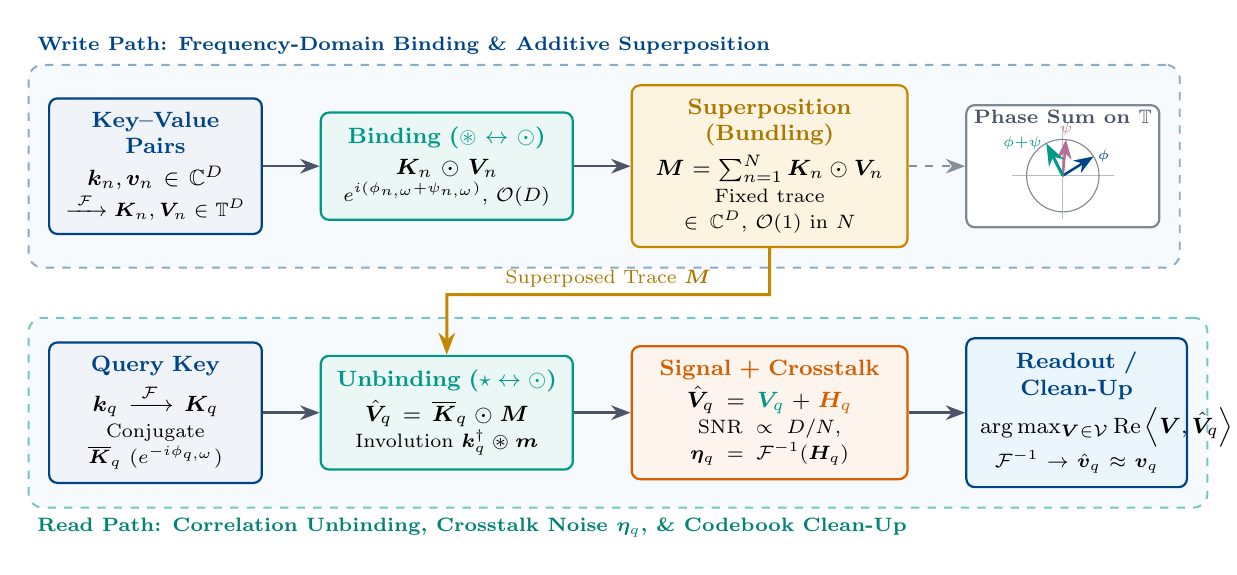
\begin{tikzpicture}[
    >=Stealth,
    node distance=0.65cm and 0.72cm,
    every node/.style={font=\footnotesize},
    box/.style={
        rectangle,
        rounded corners=3pt,
        draw=okabeSlate,
        line width=0.8pt,
        fill=white,
        align=center,
        inner sep=5pt,
        minimum height=1.25cm
    },
    inputbox/.style={
        box,
        draw=okabeNavy,
        fill=okabeNavy!6,
        text width=2.35cm
    },
    bindbox/.style={
        box,
        draw=okabeTeal,
        fill=okabeTeal!8,
        text width=2.85cm
    },
    membox/.style={
        box,
        draw=okabeAmber!85!black,
        fill=okabeAmber!12,
        text width=3.15cm
    },
    decompbox/.style={
        box,
        draw=okabeCoral,
        fill=okabeCoral!7,
        text width=3.15cm
    },
    outbox/.style={
        box,
        draw=okabeNavy,
        fill=okabeSky!12,
        text width=2.45cm
    },
    flow/.style={
        ->,
        line width=0.9pt,
        draw=okabeSlate
    },
    memflow/.style={
        ->,
        line width=1.1pt,
        draw=okabeAmber!85!black
    },
    band/.style={
        rounded corners=5pt,
        dashed,
        line width=0.7pt,
        inner sep=7pt
    }
]

% ==============================================================================
% TOP ROW: WRITE / ENFOLDING PATH (Phasor Encoding -> Binding -> Bundling)
% ==============================================================================
\node[inputbox] (inputs) {%
    \textbf{\color{okabeNavy}Key--Value Pairs}\\[2pt]
    $\vect{k}_n, \vect{v}_n \in \C^D$\\
    {\scriptsize $\xrightarrow{\;\DFT\;}\vect{K}_n, \vect{V}_n \in \mathbb{T}^D$}%
};

\node[bindbox, right=of inputs] (binding) {%
    \textbf{\color{okabeTeal}Binding ($\cconv \leftrightarrow \hadamard$)}\\[2pt]
    $\vect{K}_n \hadamard \vect{V}_n$\\
    {\scriptsize $e^{i(\phi_{n,\omega}+\psi_{n,\omega})}$, $\bigo{D}$}%
};

\node[membox, right=of binding] (bundling) {%
    \textbf{\color{okabeAmber!75!black}Superposition (Bundling)}\\[2pt]
    $\vect{M} = \sum_{n=1}^{N} \vect{K}_n \hadamard \vect{V}_n$\\
    {\scriptsize Fixed trace $\in \C^D$, $\bigo{1}$ in $N$}%
};

% Mini Unit-Circle Phasor Inset (positioned relative to bundling)
\node[box, draw=okabeSlate!70, fill=white, right=of bundling, minimum width=2.45cm, minimum height=1.55cm] (phasor_frame) {};
\begin{scope}[shift={(phasor_frame.center)}, yshift=-0.12cm]
    \draw[okabeSlate!40, thin] (-0.65,0) -- (0.65,0);
    \draw[okabeSlate!40, thin] (0,-0.55) -- (0,0.55);
    \draw[okabeSlate!70, thin] (0,0) circle (0.46cm);
    % Key phasor (navy)
    \draw[->, okabeNavy, line width=0.9pt] (0,0) -- (32:0.46cm)
        node[right, inner sep=1pt, font=\tiny, text=okabeNavy] {$\phi$};
    % Value phasor (sky/purple)
    \draw[->, okabePurple!90!black, line width=0.9pt] (0,0) -- (85:0.46cm)
        node[above, inner sep=1pt, font=\tiny, text=okabePurple!90!black] {$\psi$};
    % Bound phasor (teal)
    \draw[->, okabeTeal, line width=1.1pt] (0,0) -- (117:0.46cm)
        node[left, inner sep=1pt, font=\tiny, text=okabeTeal] {$\phi{+}\psi$};
\end{scope}
\node[anchor=north, font=\scriptsize\bfseries, text=okabeSlate, inner sep=2pt] at (phasor_frame.north) {Phase Sum on $\mathbb{T}$};

% ==============================================================================
% BOTTOM ROW: READ / UNBINDING PATH (Query -> Unbinding -> Crosstalk -> Clean-up)
% ==============================================================================
\node[inputbox, below=1.35cm of inputs] (query) {%
    \textbf{\color{okabeNavy}Query Key}\\[2pt]
    $\vect{k}_q \xrightarrow{\;\DFT\;} \vect{K}_q$\\
    {\scriptsize Conjugate $\conj{\vect{K}}_q$ ($e^{-i\phi_{q,\omega}}$)}%
};

\node[bindbox, right=of query] (unbinding) {%
    \textbf{\color{okabeTeal}Unbinding ($\ccorr \leftrightarrow \hadamard$)}\\[2pt]
    $\hat{\vect{V}}_q = \conj{\vect{K}}_q \hadamard \vect{M}$\\
    {\scriptsize Involution $\inv{\vect{k}}_q \cconv \vect{m}$}%
};

\node[decompbox, right=of unbinding] (decomp) {%
    \textbf{\color{okabeCoral}Signal + Crosstalk}\\[2pt]
    $\hat{\vect{V}}_q = {\color{okabeTeal}\vect{V}_q} + {\color{okabeCoral}\vect{H}_q}$\\
    {\scriptsize $\SNR \propto D / N$,\; $\vect{\eta}_q = \IDFT(\vect{H}_q)$}%
};

\node[outbox, right=of decomp] (cleanup) {%
    \textbf{\color{okabeNavy}Readout / Clean-Up}\\[2pt]
    $\arg\max_{\vect{V} \in \mathcal{V}} \Real\inner{\vect{V}}{\hat{\vect{V}}_q}$\\
    {\scriptsize $\IDFT \rightarrow \hat{\vect{v}}_q \approx \vect{v}_q$}%
};

% ==============================================================================
% ARROWS & ROUTING
% ==============================================================================
% Top row flows
\draw[flow] (inputs) -- (binding);
\draw[flow] (binding) -- (bundling);
\draw[flow, dashed, draw=okabeSlate!65] (bundling) -- (phasor_frame);

% Bottom row flows
\draw[flow] (query) -- (unbinding);
\draw[flow] (unbinding) -- (decomp);
\draw[flow] (decomp) -- (cleanup);

% Bridge arrow from Bundling (Write) to Unbinding (Read) through middle channel
\coordinate (mid_channel) at ($(bundling.south)!0.48!(decomp.north)$);
\draw[memflow] (bundling.south) -- (mid_channel)
    -| node[pos=0.25, above, font=\scriptsize, text=okabeAmber!75!black, inner sep=2pt]
    {Superposed Trace $\vect{M}$} (unbinding.north);

% ==============================================================================
% BACKGROUND GROUPING BANDS
% ==============================================================================
\begin{scope}[on background layer]
    \node[band, draw=okabeNavy!45, fill=okabeLightBg,
          fit=(inputs)(binding)(bundling)(phasor_frame),
          label={[anchor=south west, font=\scriptsize\bfseries, text=okabeNavy]north west:Write Path: Frequency-Domain Binding \& Additive Superposition}] (write_band) {};
    \node[band, draw=okabeTeal!55, fill=okabeLightBg,
          fit=(query)(unbinding)(decomp)(cleanup),
          label={[anchor=north west, font=\scriptsize\bfseries, text=okabeTeal!85!black]south west:Read Path: Correlation Unbinding, Crosstalk Noise $\vect{\eta}_q$, \& Codebook Clean-Up}] (read_band) {};
\end{scope}

\end{tikzpicture}
 inside a figure environment.
% Requires TikZ libraries: positioning, arrows.meta, shapes.geometric, fit, calc,
% backgrounds; and Okabe-Ito colors + math macros from main.tex.
% ==============================================================================
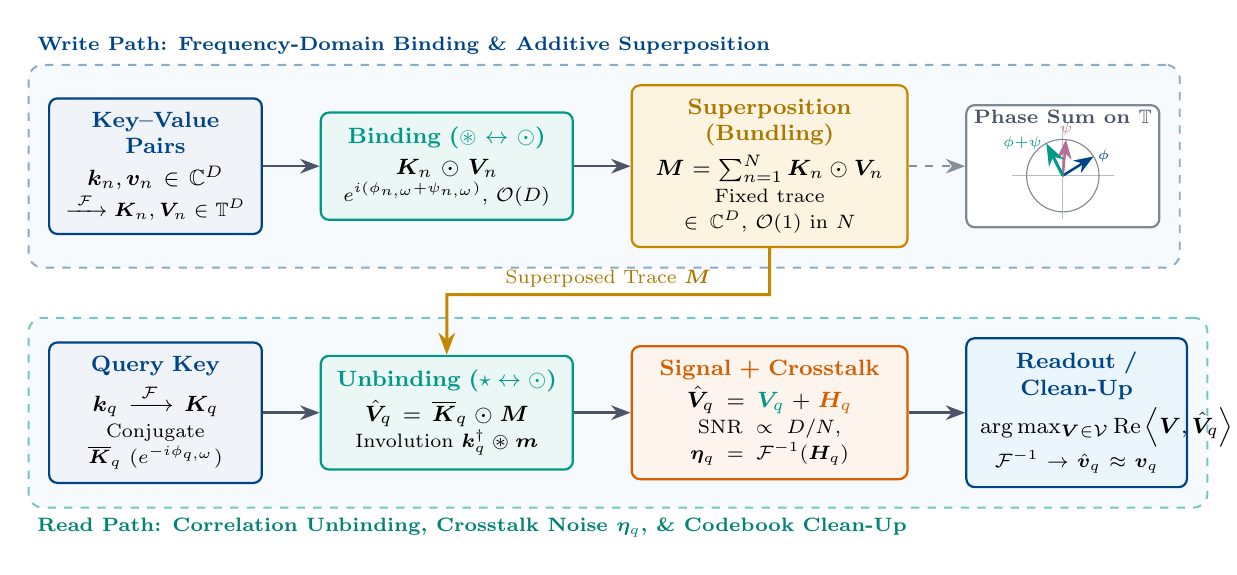
\begin{tikzpicture}[
    >=Stealth,
    node distance=0.65cm and 0.72cm,
    every node/.style={font=\footnotesize},
    box/.style={
        rectangle,
        rounded corners=3pt,
        draw=okabeSlate,
        line width=0.8pt,
        fill=white,
        align=center,
        inner sep=5pt,
        minimum height=1.25cm
    },
    inputbox/.style={
        box,
        draw=okabeNavy,
        fill=okabeNavy!6,
        text width=2.35cm
    },
    bindbox/.style={
        box,
        draw=okabeTeal,
        fill=okabeTeal!8,
        text width=2.85cm
    },
    membox/.style={
        box,
        draw=okabeAmber!85!black,
        fill=okabeAmber!12,
        text width=3.15cm
    },
    decompbox/.style={
        box,
        draw=okabeCoral,
        fill=okabeCoral!7,
        text width=3.15cm
    },
    outbox/.style={
        box,
        draw=okabeNavy,
        fill=okabeSky!12,
        text width=2.45cm
    },
    flow/.style={
        ->,
        line width=0.9pt,
        draw=okabeSlate
    },
    memflow/.style={
        ->,
        line width=1.1pt,
        draw=okabeAmber!85!black
    },
    band/.style={
        rounded corners=5pt,
        dashed,
        line width=0.7pt,
        inner sep=7pt
    }
]

% ==============================================================================
% TOP ROW: WRITE / ENFOLDING PATH (Phasor Encoding -> Binding -> Bundling)
% ==============================================================================
\node[inputbox] (inputs) {%
    \textbf{\color{okabeNavy}Key--Value Pairs}\\[2pt]
    $\vect{k}_n, \vect{v}_n \in \C^D$\\
    {\scriptsize $\xrightarrow{\;\DFT\;}\vect{K}_n, \vect{V}_n \in \mathbb{T}^D$}%
};

\node[bindbox, right=of inputs] (binding) {%
    \textbf{\color{okabeTeal}Binding ($\cconv \leftrightarrow \hadamard$)}\\[2pt]
    $\vect{K}_n \hadamard \vect{V}_n$\\
    {\scriptsize $e^{i(\phi_{n,\omega}+\psi_{n,\omega})}$, $\bigo{D}$}%
};

\node[membox, right=of binding] (bundling) {%
    \textbf{\color{okabeAmber!75!black}Superposition (Bundling)}\\[2pt]
    $\vect{M} = \sum_{n=1}^{N} \vect{K}_n \hadamard \vect{V}_n$\\
    {\scriptsize Fixed trace $\in \C^D$, $\bigo{1}$ in $N$}%
};

% Mini Unit-Circle Phasor Inset (positioned relative to bundling)
\node[box, draw=okabeSlate!70, fill=white, right=of bundling, minimum width=2.45cm, minimum height=1.55cm] (phasor_frame) {};
\begin{scope}[shift={(phasor_frame.center)}, yshift=-0.12cm]
    \draw[okabeSlate!40, thin] (-0.65,0) -- (0.65,0);
    \draw[okabeSlate!40, thin] (0,-0.55) -- (0,0.55);
    \draw[okabeSlate!70, thin] (0,0) circle (0.46cm);
    % Key phasor (navy)
    \draw[->, okabeNavy, line width=0.9pt] (0,0) -- (32:0.46cm)
        node[right, inner sep=1pt, font=\tiny, text=okabeNavy] {$\phi$};
    % Value phasor (sky/purple)
    \draw[->, okabePurple!90!black, line width=0.9pt] (0,0) -- (85:0.46cm)
        node[above, inner sep=1pt, font=\tiny, text=okabePurple!90!black] {$\psi$};
    % Bound phasor (teal)
    \draw[->, okabeTeal, line width=1.1pt] (0,0) -- (117:0.46cm)
        node[left, inner sep=1pt, font=\tiny, text=okabeTeal] {$\phi{+}\psi$};
\end{scope}
\node[anchor=north, font=\scriptsize\bfseries, text=okabeSlate, inner sep=2pt] at (phasor_frame.north) {Phase Sum on $\mathbb{T}$};

% ==============================================================================
% BOTTOM ROW: READ / UNBINDING PATH (Query -> Unbinding -> Crosstalk -> Clean-up)
% ==============================================================================
\node[inputbox, below=1.35cm of inputs] (query) {%
    \textbf{\color{okabeNavy}Query Key}\\[2pt]
    $\vect{k}_q \xrightarrow{\;\DFT\;} \vect{K}_q$\\
    {\scriptsize Conjugate $\conj{\vect{K}}_q$ ($e^{-i\phi_{q,\omega}}$)}%
};

\node[bindbox, right=of query] (unbinding) {%
    \textbf{\color{okabeTeal}Unbinding ($\ccorr \leftrightarrow \hadamard$)}\\[2pt]
    $\hat{\vect{V}}_q = \conj{\vect{K}}_q \hadamard \vect{M}$\\
    {\scriptsize Involution $\inv{\vect{k}}_q \cconv \vect{m}$}%
};

\node[decompbox, right=of unbinding] (decomp) {%
    \textbf{\color{okabeCoral}Signal + Crosstalk}\\[2pt]
    $\hat{\vect{V}}_q = {\color{okabeTeal}\vect{V}_q} + {\color{okabeCoral}\vect{H}_q}$\\
    {\scriptsize $\SNR \propto D / N$,\; $\vect{\eta}_q = \IDFT(\vect{H}_q)$}%
};

\node[outbox, right=of decomp] (cleanup) {%
    \textbf{\color{okabeNavy}Readout / Clean-Up}\\[2pt]
    $\arg\max_{\vect{V} \in \mathcal{V}} \Real\inner{\vect{V}}{\hat{\vect{V}}_q}$\\
    {\scriptsize $\IDFT \rightarrow \hat{\vect{v}}_q \approx \vect{v}_q$}%
};

% ==============================================================================
% ARROWS & ROUTING
% ==============================================================================
% Top row flows
\draw[flow] (inputs) -- (binding);
\draw[flow] (binding) -- (bundling);
\draw[flow, dashed, draw=okabeSlate!65] (bundling) -- (phasor_frame);

% Bottom row flows
\draw[flow] (query) -- (unbinding);
\draw[flow] (unbinding) -- (decomp);
\draw[flow] (decomp) -- (cleanup);

% Bridge arrow from Bundling (Write) to Unbinding (Read) through middle channel
\coordinate (mid_channel) at ($(bundling.south)!0.48!(decomp.north)$);
\draw[memflow] (bundling.south) -- (mid_channel)
    -| node[pos=0.25, above, font=\scriptsize, text=okabeAmber!75!black, inner sep=2pt]
    {Superposed Trace $\vect{M}$} (unbinding.north);

% ==============================================================================
% BACKGROUND GROUPING BANDS
% ==============================================================================
\begin{scope}[on background layer]
    \node[band, draw=okabeNavy!45, fill=okabeLightBg,
          fit=(inputs)(binding)(bundling)(phasor_frame),
          label={[anchor=south west, font=\scriptsize\bfseries, text=okabeNavy]north west:Write Path: Frequency-Domain Binding \& Additive Superposition}] (write_band) {};
    \node[band, draw=okabeTeal!55, fill=okabeLightBg,
          fit=(query)(unbinding)(decomp)(cleanup),
          label={[anchor=north west, font=\scriptsize\bfseries, text=okabeTeal!85!black]south west:Read Path: Correlation Unbinding, Crosstalk Noise $\vect{\eta}_q$, \& Codebook Clean-Up}] (read_band) {};
\end{scope}

\end{tikzpicture}

    \caption{Algebraic operations in complex phase space $\C^D$. \emph{Top (Write Path):} Key--value pairs $(\vect{k}_n, \vect{v}_n)$ are transformed into phasors $(\vect{K}_n, \vect{V}_n) \in \mathbb{T}^D$, bound via elementwise Hadamard phase addition ($\cconv \leftrightarrow \hadamard$), and superposed into a single constant-size trace $\vect{M}$. \emph{Bottom (Read Path):} Querying $\vect{M}$ with the phase conjugate $\conj{\vect{K}}_q$ executes circular correlation $\ccorr$, recovering the exact target signal $\vect{V}_q$ perturbed by additive crosstalk $\vect{H}_q$ (time-domain $\vect{\eta}_q$), which is subsequently denoised against a codebook $\mathcal{V}$ via clean-up readout.}
    \label{fig:algebra}
\end{figure}

\begin{remark}[Relation to Sutherland's Complex Correlation Matrix]\label{rem:sutherland_matrix}
In classical 1990s HNNs~\cite{SUTHERLAND_1990_HNN}, stimulus--response associations $\{(\vect{k}_n, \vect{v}_n)\}_{n=1}^N$ with $\vect{k}_n \in \C^{D_k}$ and $\vect{v}_n \in \C^{D_v}$ are enfolded into a full complex outer-product correlation matrix $\mat{X} = \sum_{n=1}^{N} \vect{v}_n \vect{k}_n\herm \in \C^{D_v \times D_k}$, and recalled via linear projection:
\begin{equation}\label{eq:sutherland_recall}
    \hat{\vect{v}}_q = \frac{1}{\norm{\vect{k}_q}_2^2} \mat{X} \vect{k}_q
    = \vect{v}_q + \sum_{\substack{n=1 \\ n \neq q}}^{N} \frac{\inner{\vect{k}_n}{\vect{k}_q}}{\norm{\vect{k}_q}_2^2} \vect{v}_n.
\end{equation}
Comparing~\eqref{eq:sutherland_recall} with~\eqref{eq:unbinding_decomposition}, circular convolution binding restricts the $\bigo{D^2}$ dense correlation matrix $\mat{X}$ to a circulant linear operator parameterized by just $\bigo{D}$ numbers (the vector $\vect{m}$), trading $\bigo{D}$ storage reduction for an extra factor of $D$ reduction in total matrix capacity while preserving the identical additive crosstalk structure.
\end{remark}

% ------------------------------------------------------------------------------
\subsection{Crosstalk Noise Analysis and Capacity Bounds}\label{sec:math:capacity}
% ------------------------------------------------------------------------------

Because $N$ bound pairs share the same $D$-dimensional substrate, retrieval accuracy is governed by the statistical balance between the coherent target signal and the incoherent crosstalk term $\vect{\eta}_q$ (or $\vect{H}_q$).
We now derive exact second-order moments, the $\SNR$ scaling law, and the resulting clean-up retrieval capacity bound~\cite{PLATE_1995_HRR,FRADY_CAPACITY_VSA}.

\begin{theorem}[Crosstalk Statistics and $\SNR$ Scaling Law]\label{thm:snr_capacity}
Suppose $N \ge 1$ key--value pairs are stored via uniform superposition in a $D$-dimensional holographic trace, and retrieval is queried with key $q \in \{1, \dots, N\}$ and scored against both the ground-truth value and an independent distractor item from a codebook $\mathcal{V}$.
\begin{enumerate}
    \item \textbf{Unitary Complex Phasors (FHRR on $\mathbb{T}^D$):}
    Let $\{\vect{K}_n\}_{n=1}^N$, $\{\vect{V}_n\}_{n=1}^N$, and an unstored distractor $\vect{V}' \notin \{\vect{V}_n\}_{n=1}^N$ be mutually independent on $\mathbb{T}^D$ with i.i.d.\ uniform phases in $[-\pi, \pi)$.
    Define the match score $S_q \coloneqq s(\vect{V}_q, \hat{\vect{V}}_q) = \frac{1}{D}\Real\inner{\vect{V}_q}{\hat{\vect{V}}_q}$ and distractor score $S' \coloneqq s(\vect{V}', \hat{\vect{V}}_q)$.
    Then $S_q$ and $S'$ are uncorrelated with exact moments
    \begin{align}
        \E[S_q] &= 1, & \Var(S_q) &= \frac{N - 1}{2D}, \label{eq:fhrr_match_var} \\
        \E[S'] &= 0, & \Var(S') &= \frac{N}{2D}. \label{eq:fhrr_distractor_var}
    \end{align}
    Consequently, the target-retrieval and discrimination signal-to-noise ratios satisfy
    \begin{equation}\label{eq:snr_fhrr}
        \SNR_{\mathrm{FHRR}}^{\mathrm{match}}
        \coloneqq \frac{\E[S_q]^2}{\Var(S_q)} = \frac{2D}{N - 1},
        \qquad
        \SNR_{\mathrm{FHRR}}^{\mathrm{disc}}
        \coloneqq \frac{\left(\E[S_q] - \E[S']\right)^2}{\Var(S_q - S')} = \frac{2D}{2N - 1}.
    \end{equation}

    \item \textbf{Real-Valued Gaussian HRR ($\R^D$):}
    Let $\{\vect{k}_n\}_{n=1}^N$, $\{\vect{v}_n\}_{n=1}^N$, and an unstored distractor $\vect{v}' \notin \{\vect{v}_n\}_{n=1}^N$ be mutually independent in $\R^D$ with i.i.d.\ entries drawn from $\mathcal{N}(0, D^{-1})$, and define $S_q^{\R} \coloneqq \inner{\vect{v}_q}{\hat{\vect{v}}_q}$ and $S'^{\R} \coloneqq \inner{\vect{v}'}{\hat{\vect{v}}_q}$.
    Then $\E[S_q^{\R}] = 1$, $\E[S'^{\R}] = 0$, and
    \begin{equation}\label{eq:hrr_vars}
        \Var\!\left(S_q^{\R}\right) = \frac{N + 5}{D} + \bigo{D^{-2}},
        \qquad
        \Var\!\left(S'^{\R}\right) = \frac{N + 1}{D} + \bigo{D^{-2}},
    \end{equation}
    yielding the discrimination scaling
    \begin{equation}\label{eq:snr_hrr}
        \SNR_{\mathrm{HRR}}^{\mathrm{disc}}
        = \frac{D}{2N + 6 + \bigo{D^{-1}}} \;\sim\; \frac{D}{2N}.
    \end{equation}
\end{enumerate}
In both regimes, $\SNR = \Theta(D/N)$, scaling linearly with vector dimensionality $D$ and inversely with the superposition load $N$.
\end{theorem}

\begin{proof}
\emph{Part 1 (Unitary FHRR).}
Because $\abs{K_{q,\omega}} = 1$, the frequency-domain unbinding~\eqref{eq:unbinding_freq} yields $\hat{\vect{V}}_q = \vect{V}_q + \vect{H}_q$, where $H_{q,\omega} = \sum_{n \neq q} e^{i(\phi_{n,\omega} - \phi_{q,\omega} + \psi_{n,\omega})}$.
Evaluating the normalized match similarity~\eqref{eq:phasor_similarity} gives
\begin{equation}\label{eq:fhrr_sq_expand}
    S_q = \frac{1}{D}\Real\inner{\vect{V}_q}{\vect{V}_q + \vect{H}_q}
    = 1 + \frac{1}{D} \sum_{\omega=0}^{D-1} \sum_{\substack{n=1 \\ n \neq q}}^{N} \cos\!\left(\Delta_{q,n,\omega}\right),
\end{equation}
where $\Delta_{q,n,\omega} = \left(\phi_{n,\omega} - \phi_{q,\omega} + \psi_{n,\omega} - \psi_{q,\omega}\right) \bmod 2\pi$.
Conditioned on $(\vect{K}_q, \vect{V}_q)$, shifting i.i.d.\ uniform angles $(\phi_{n,\omega} + \psi_{n,\omega}) \bmod 2\pi$ by the fixed offset $-(\phi_{q,\omega} + \psi_{q,\omega})$ leaves the $D(N-1)$ random variables $\{\Delta_{q,n,\omega}\}$ mutually independent and uniform on $[-\pi, \pi)$---hence also unconditionally independent of $(\vect{K}_q, \vect{V}_q)$.
Since $\E[\cos\Delta_{q,n,\omega}] = 0$ and $\Var(\cos\Delta_{q,n,\omega}) = \frac{1}{2}$, we obtain $\E[S_q] = 1$ and
\begin{equation*}
    \Var(S_q) = \frac{1}{D^2} \cdot D(N - 1) \cdot \frac{1}{2} = \frac{N - 1}{2D}.
\end{equation*}
For an independent distractor $\vect{V}' \in \mathbb{T}^D$ with phases $\psi'_\omega$, the overlap decomposes into $DN$ independent uniform-phase cosine terms:
\begin{equation*}
    S' = \frac{1}{D}\sum_{\omega=0}^{D-1} \cos(\psi_{q,\omega} - \psi'_\omega)
       + \frac{1}{D}\sum_{\omega=0}^{D-1}\sum_{n \neq q} \cos\!\left(\phi_{n,\omega} - \phi_{q,\omega} + \psi_{n,\omega} - \psi'_\omega\right),
\end{equation*}
giving $\E[S'] = 0$ and $\Var(S') = \frac{DN}{2D^2} = \frac{N}{2D}$.
To verify $\operatorname{Cov}(S_q, S') = 0$, note that for each $(n, \omega)$ with $n \neq q$, setting $\alpha = \phi_{n,\omega} - \phi_{q,\omega} + \psi_{n,\omega}$ yields
\begin{equation*}
    \E\!\left[\cos(\alpha - \psi_{q,\omega})\cos(\alpha - \psi'_\omega)\right]
    = \frac{1}{2}\E\!\left[\cos(\psi'_\omega - \psi_{q,\omega})\right]
    + \frac{1}{2}\E\!\left[\cos(2\alpha - \psi_{q,\omega} - \psi'_\omega)\right]
    = 0,
\end{equation*}
because $\psi'_\omega$ is independent of both $\psi_{q,\omega}$ and $\alpha$.
Hence $\Var(S_q - S') = \Var(S_q) + \Var(S') = \frac{2N - 1}{2D}$, establishing~\eqref{eq:snr_fhrr}.

\medskip
\noindent\emph{Part 2 (Real Gaussian HRR).}
By Lemma~\ref{lem:ccorr_props}(3), the real match score splits into a self-energy term and $N-1$ crosstalk inner products:
\begin{equation*}
    S_q^{\R} = \norm{\vect{w}_q}_2^2 + \sum_{n \neq q} \inner{\vect{w}_q}{\vect{w}_n},
    \qquad \vect{w}_n \coloneqq \vect{k}_n \cconv \vect{v}_n.
\end{equation*}
For i.i.d.\ entries $k_{n,r}, v_{n,r} \sim \mathcal{N}(0, D^{-1})$, each coordinate $w_{n,j} = \sum_{r=0}^{D-1} k_{n,r} v_{n,(j-r)\bmod D}$ has mean $0$ and covariance $\E[w_{n,j} w_{n,j'}] = D^{-1}\delta_{j,j'}$.
Thus $\E[\norm{\vect{w}_q}_2^2] = 1$, and by independence across $n$, each crosstalk term $C_n = \inner{\vect{w}_q}{\vect{w}_n}$ ($n \neq q$) satisfies $\E[C_n] = 0$, $\operatorname{Cov}(C_n, C_{n'}) = 0$ for $n \neq n'$, and
\begin{equation*}
    \Var(C_n) = \E\!\left[\vect{w}_q\trans \E[\vect{w}_n \vect{w}_n\trans] \vect{w}_q\right]
    = \frac{1}{D}\E\!\left[\norm{\vect{w}_q}_2^2\right] = \frac{1}{D}.
\end{equation*}
To evaluate the self-term variance $\Var(\norm{\vect{w}_q}_2^2)$, we apply Parseval's identity: $\norm{\vect{w}_q}_2^2 = \frac{1}{D}\sum_{\omega=0}^{D-1} \abs{K_{q,\omega}}^2 \abs{V_{q,\omega}}^2$.
Because $\vect{k}_q, \vect{v}_q \in \R^D$ are real Gaussian with variance $D^{-1}$, their DFT coefficients satisfy conjugate symmetry ($K_{q,D-\omega} = \conj{K}_{q,\omega}$) and are independent across $\omega \in \{0, \dots, \lfloor D/2 \rfloor\}$.
For every interior frequency $1 \le \omega < D/2$, $K_{q,\omega}, V_{q,\omega} \sim \mathcal{CN}(0, 1)$, so $\abs{K_{q,\omega}}^2, \abs{V_{q,\omega}}^2 \overset{\text{i.i.d.}}{\sim} \mathrm{Exp}(1)$ with $\E[\abs{K_{q,\omega}}^4] = 2$.
Each conjugate pair $\{\omega, D-\omega\}$ therefore contributes $2\abs{K_{q,\omega}}^2\abs{V_{q,\omega}}^2$ with variance $4(2\cdot 2 - 1) = 12$.
Together with the real DC (and Nyquist, if $D$ is even) terms of variance $3\cdot 3 - 1 = 8$, summing over all $D$ bins yields Plate's exact parity-dependent finite-$D$ variance~\cite{PLATE_1995_HRR},
\begin{equation*}
    \Var\!\left(\norm{\vect{w}_q}_2^2\right) = \frac{6}{D} + \frac{2 + 2\,\mathbf{1}_{\{D\text{ even}\}}}{D^2} = \frac{6}{D} + \bigo{D^{-2}}.
\end{equation*}
Adding the $N-1$ uncorrelated crosstalk variances $\frac{N-1}{D}$ yields $\Var(S_q^{\R}) = \frac{N + 5}{D} + \frac{2 + 2\,\mathbf{1}_{\{D\text{ even}\}}}{D^2}$.
Finally, for an independent distractor $\vect{v}' \sim \mathcal{N}(\vect{0}, D^{-1}\mat{I}_D)$, $\E[S'^{\R}] = 0$ and $\Var(S'^{\R}) = \frac{1}{D}\E[\norm{\hat{\vect{v}}_q}_2^2]$.
Using~\eqref{eq:unbinding_freq}, interior complex bins satisfy $\E[\abs{\hat{V}_{q,\omega}}^2] = \E[\abs{K_{q,\omega}}^4]\E[\abs{V_{q,\omega}}^2] + (N-1)\cdot 1 = N + 1$ whereas the real DC/Nyquist bins satisfy $\E[\hat{V}_{q,\omega}^2] = N + 2$, giving the exact finite-$D$ form $\Var(S'^{\R}) = \frac{N+1}{D} + \frac{1 + \mathbf{1}_{\{D\text{ even}\}}}{D^2} = \frac{N+1}{D} + \bigo{D^{-2}}$~\cite{PLATE_1995_HRR}.
Combining the uncorrelated scores $S_q^{\R}$ and $S'^{\R}$ produces~\eqref{eq:snr_hrr}.
\end{proof}

Two insights---along with their precise scope conditions---follow from Theorem~\ref{thm:snr_capacity}.
First, unitary complex phasors (FHRR) achieve a \emph{factor-of-two discrimination $\SNR$ advantage} over real Gaussian HRR at equal ambient dimensionality $D$ ($\frac{D}{N}$ vs.\ $\frac{D}{2N}$), despite requiring only $D$ real phase parameters on $\mathbb{T}^D$: unitary keys eliminate spectral self-distortion completely, while taking the real part in~\eqref{eq:phasor_similarity} rejects the orthogonal imaginary quadrature component of isotropic complex crosstalk noise.
Crucially, this factor-of-two ($3\,\mathrm{dB}$) gain holds \emph{conditionally under equal expected unit-energy normalization} ($\frac{1}{D}\norm{\vect{V}}_2^2 = 1$ on $\mathbb{T}^D$ matched to $\E[\norm{\vect{v}}_2^2] = 1$ in $\R^D$), \emph{i.i.d.\ circular-symmetric complex-phasor and isotropic real-Gaussian independence assumptions}, and the \emph{phase-coherent real-part readout}~\eqref{eq:phasor_similarity}---not unconditionally across arbitrary score definitions (such as phase-agnostic modulus scoring $\abs{\inner{\vect{V}_q}{\hat{\vect{V}}_q}}$), non-unitary complex keys, or correlated learned embeddings.
Second, because $\Var(S_q)$ grows linearly with $N$, a raw unbound vector $\hat{\vect{V}}_q$ is intrinsically noisy; exact symbol recovery therefore relies on a \emph{clean-up memory}---a nearest-neighbor projection onto a known codebook $\mathcal{V} = \{\vect{V}^{(1)}, \dots, \vect{V}^{(M)}\}$ (implemented via dot-product search, Hopfield attractors, or iterative resonator networks).

\begin{corollary}[Asymptotic Clean-Up Retrieval Capacity]\label{cor:cleanup_capacity}
Let $\mathcal{V} \subset \mathbb{T}^D$ be a random codebook of $M \ge N$ mutually independent i.i.d.\ uniform-phase codewords, and suppose a unitary FHRR trace superposes $N$ mutually independent keys $\{\vect{K}_n\}_{n=1}^N \subset \mathbb{T}^D$ bound to $N$ distinct values $\{\vect{V}_n\}_{n=1}^N$ sampled without replacement from $\mathcal{V}$.
Consider retrieving a queried value $\vect{V}_q$ via maximum-similarity clean-up, $\hat{\vect{V}}_{\mathrm{clean}} = \arg\max_{\vect{V} \in \mathcal{V}} s(\vect{V}, \hat{\vect{V}}_q)$.
Under the asymptotic high-dimensional Gaussian (CLT) approximation ($D \gg 1$ with $\ln M = o(D)$), the probability of misretrieval $P_{\mathrm{err}} = \Pr(\hat{\vect{V}}_{\mathrm{clean}} \neq \vect{V}_q)$ is approximated and conservatively upper-bounded by
\begin{equation}\label{eq:perr_bound}
    P_{\mathrm{err}} \lesssim \frac{M - 1}{2} \exp\!\left(-\frac{D}{2N - 1}\right).
\end{equation}
Consequently, targeting $P_{\mathrm{err}} \le \delta$ for any desired error rate $\delta \in (0, 1)$ yields the asymptotic capacity scaling
\begin{equation}\label{eq:capacity_bound}
    N_{\max}(D, M, \delta) \approx \frac{D}{2 \ln\!\left(\frac{M - 1}{2\delta}\right)} + \frac{1}{2}
    = \Theta\!\left(\frac{D}{\ln(M / \delta)}\right).
\end{equation}
\end{corollary}

\begin{proof}
By the union bound over the $M - 1$ non-target codebook items $\vect{V}^{(m)} \neq \vect{V}_q$,
\begin{equation*}
    P_{\mathrm{err}} = \Pr\!\left(\bigcup_{m \neq q} \left\{ S^{(m)} \ge S_q \right\}\right)
    \le \sum_{m \neq q} \Pr\!\left(S_q - S^{(m)} \le 0\right).
\end{equation*}
Under mutual independence and distinct-value sampling ($\vect{V}_{n^*} \neq \vect{V}_q$ for $n^* \neq q$), the score statistics and zero-covariance property $\operatorname{Cov}(S_q, S^{(m)}) = 0$ hold identically whether $\vect{V}^{(m)}$ is one of the $M - N$ unstored distractors or one of the $N - 1$ in-bundle distractors $\vect{V}_{n^*}$ ($n^* \neq q$), because the self-key residual $e^{i(\phi_{n^*,\omega} - \phi_{q,\omega} + \psi_{n^*,\omega} - \psi_{n^*,\omega})} = e^{i(\phi_{n^*,\omega} - \phi_{q,\omega})}$ retains an independent uniform phase while remaining uncorrelated with $\psi_{n^*,\omega} - \psi_{q,\omega}$.
For $D \gg 1$, the Central Limit Theorem implies $S_q - S^{(m)} \overset{d}{\approx} \mathcal{N}\!\left(1, \sigma_\Delta^2\right)$ with $\sigma_\Delta^2 = \Var(S_q - S^{(m)}) = \frac{2N - 1}{2D}$ from Theorem~\ref{thm:snr_capacity}.
Applying the standard Gaussian tail bound $\Phi(-z) \le \frac{1}{2}e^{-z^2/2}$ at $z = \sigma_\Delta^{-1} = \sqrt{\frac{2D}{2N - 1}}$ gives
\begin{equation*}
    \Pr\!\left(S_q - S^{(m)} \le 0\right)
    \approx \Phi\!\left(-\frac{1}{\sigma_\Delta}\right)
    \le \frac{1}{2} \exp\!\left(-\frac{1}{2\sigma_\Delta^2}\right)
    = \frac{1}{2} \exp\!\left(-\frac{D}{2N - 1}\right).
\end{equation*}
Multiplying by $M - 1$ yields~\eqref{eq:perr_bound}, and solving $\frac{M-1}{2}\exp\!\left(-\frac{D}{2N-1}\right) \le \delta$ for $N$ produces~\eqref{eq:capacity_bound}.
(Note that~\eqref{eq:perr_bound}--\eqref{eq:capacity_bound} are conservative in two respects: $\Phi(-z) \le \frac{1}{2}e^{-z^2/2}$ carries a factor-of-$1/2$ pre-exponential constant rather than Mills' ratio $(\sqrt{2\pi}\,z)^{-1}$, and applying a union bound across pairwise events $\{S^{(m)} \ge S_q\}$ that share $S_q$ introduces up to a factor-of-$2$ conservatism in~\eqref{eq:capacity_bound} for large $M$ relative to the conditional extreme-value retrieval integral $P_{\mathrm{err}} = 1 - \E_{S_q}\!\bigl[\Phi(S_q / \sigma_d)^{M-1}\bigr]$ of Frady et al.~\cite{FRADY_CAPACITY_VSA}, under which $N_{\max} \sim D / \bigl(\sqrt{\ln M} + \sqrt{\ln(1/\delta)}\bigr)^2$.)
\end{proof}

Corollary~\ref{cor:cleanup_capacity} highlights a logarithmic resilience to dictionary size: storing $N$ structured bindings reliably requires dimension $D$ to grow only \emph{linearly} in $N$ and \emph{logarithmically} in codebook size $M$.
For instance, at $D = 4096$, the asymptotic estimate~\eqref{eq:capacity_bound} indicates that a single unitary phasor trace can superpose $N \approx 100$ key--value bindings drawn from a vocabulary of $M = 10^5$ symbols with per-query error probability below $10^{-3}$.
We emphasize, however, that~\eqref{eq:perr_bound}--\eqref{eq:capacity_bound} are \emph{asymptotic high-dimensional Gaussian approximations} derived via the Central Limit Theorem rather than unconditional finite-sample concentration guarantees: at small $D$ or extreme codebook sizes where tail probabilities probe the non-Gaussian support of bounded cosine sums, rigorous finite-sample bounds require non-asymptotic Chernoff/Hoeffding or Berry--Esseen corrections with looser constants.

Equally important, this asymptotic capacity scaling rests critically on key quasi-orthogonality ($\E[\inner{\vect{K}_n}{\vect{K}_q}] = 0$).
When keys are learned end-to-end by deep neural encoders rather than sampled i.i.d., semantic clustering introduces non-zero cross-correlations $\rho_{qn} = s(\vect{K}_q, \vect{K}_n) \neq 0$, injecting a coherent bias $\sum_{n \neq q} \rho_{qn} \vect{V}_n$ whose interference power scales as $\bigo{N^2 \bar{\rho}^2}$ alongside the $\bigo{N/D}$ incoherent crosstalk variance.
Consequently, correlated keys depress the effective discrimination $\SNR$ strictly below the i.i.d.\ $(N/D)^{-1}$ upper envelope and accelerate retrieval-error growth well before the theoretical ceiling $N_{\max}$.
Mitigating correlated-key interference---through spectral whitening, phase-orthogonalization regularizers, or iterative error-correcting updates (analogous to Delta-rule / Sutherland iterative folding)---remains a central algorithmic bridge between classical VSA theory and modern deep learning, as examined in Sections~\ref{sec:history} and~\ref{sec:potentials}.
Figure~\ref{fig:capacity} corroborates Theorem~\ref{thm:snr_capacity} empirically via Monte Carlo simulation across dimensions $D \in \{256, 1024, 4096\}$ (full reproducible script provided in Appendix~\ref{app:simulation}) and juxtaposes the resulting capacity law against the memory-footprint scaling of classical HNNs, KV-caches, and dense self-attention; since clean-up error scales exponentially in $-\frac{1}{2}\SNR^{\mathrm{disc}}$ via~\eqref{eq:perr_bound}, the $2\times$ vertical $\SNR$ separation in panel~(a) directly translates into roughly double the reliable superposition load $N_{\max}$ at fixed $(D, M, \delta)$.

\begin{figure}[tbp]
    \centering
    % ==============================================================================
% figures/fig_capacity.tex
% Theoretical Capacity & Scaling Trade-offs (PGFPlots two-panel figure)
% Left panel : Analytical SNR ~ D/N curves + Monte Carlo points from
%              figures/capacity_snr.dat (generated by figures/simulate_capacity.py).
% Right panel: Memory footprint scaling (O(1) trace vs. O(D^2) HNN matrix vs.
%              O(ND) KV-cache vs. O(N^2) dense attention at D = 4096).
% Requires: pgfplots (compat=1.18), \usepgfplotslibrary{groupplots}, Okabe-Ito
%           colors, and math macros from main.tex.
% ==============================================================================
\begin{tikzpicture}
\begin{groupplot}[
    group style={
        group size=2 by 1,
        horizontal sep=1.55cm
    },
    width=0.47\textwidth,
    height=5.9cm,
    grid=both,
    major grid style={okabeSlate!22, line width=0.4pt},
    minor grid style={okabeSlate!10, line width=0.25pt},
    tick label style={font=\scriptsize},
    label style={font=\footnotesize},
    title style={font=\footnotesize\bfseries, yshift=-2pt},
    legend style={
        font=\tiny,
        fill=white,
        fill opacity=0.9,
        text opacity=1,
        draw=okabeSlate!40,
        inner sep=2pt,
        row sep=-1pt
    },
    filter discard warning=false
]

% ==============================================================================
% PANEL (a): Discrimination SNR vs. Load Ratio N/D
% ==============================================================================
\nextgroupplot[
    xmode=log,
    ymode=log,
    log basis x=10,
    log basis y=10,
    xmin=2.8e-3, xmax=0.72,
    ymin=0.65, ymax=520,
    xlabel={Superposition Load Ratio $N / D$},
    ylabel={Discrimination $\SNR^{\mathrm{disc}}$},
    title={(a) $\SNR$ Scaling: Theory vs.\ Monte Carlo},
    legend pos=south west,
    legend cell align={left}
]

% Analytical asymptotes from Theorem 2.6
\addplot[okabeTeal, line width=1.1pt, domain=3.2e-3:0.65, samples=60] {1/x};
\addlegendentry{FHRR asymptote $(N/D)^{-1}$}

\addplot[okabeCoral, line width=1.1pt, dashed, domain=3.2e-3:0.65, samples=60] {0.5/x};
\addlegendentry{HRR asymptote $\tfrac{1}{2}(N/D)^{-1}$}

% Monte Carlo data points: Unitary FHRR (open/tinted teal markers)
\addplot[
    only marks, mark=o, mark size=1.9pt,
    draw=okabeTeal, fill=white, line width=0.75pt
] table[
    x=load_ratio, y=snr_fhrr_emp,
    restrict expr to domain={\thisrow{D}}{256:256}
] {figures/capacity_snr.dat};
\addlegendentry{FHRR MC ($D=256$)}

\addplot[
    only marks, mark=square, mark size=1.8pt,
    draw=okabeTeal!85!black, fill=white, line width=0.75pt
] table[
    x=load_ratio, y=snr_fhrr_emp,
    restrict expr to domain={\thisrow{D}}{1024:1024}
] {figures/capacity_snr.dat};
\addlegendentry{FHRR MC ($D=1024$)}

\addplot[
    only marks, mark=triangle, mark size=2.1pt,
    draw=okabeNavy, fill=white, line width=0.75pt
] table[
    x=load_ratio, y=snr_fhrr_emp,
    restrict expr to domain={\thisrow{D}}{4096:4096}
] {figures/capacity_snr.dat};
\addlegendentry{FHRR MC ($D=4096$)}

% Monte Carlo data points: Real Gaussian HRR (filled coral markers)
\addplot[
    only marks, mark=*, mark size=1.5pt,
    draw=okabeCoral, fill=okabeCoral
] table[
    x=load_ratio, y=snr_hrr_emp,
    restrict expr to domain={\thisrow{D}}{256:256}
] {figures/capacity_snr.dat};
\addlegendentry{HRR MC ($D=256$)}

\addplot[
    only marks, mark=square*, mark size=1.4pt,
    draw=okabeCoral!80!black, fill=okabeCoral!80!black
] table[
    x=load_ratio, y=snr_hrr_emp,
    restrict expr to domain={\thisrow{D}}{1024:1024}
] {figures/capacity_snr.dat};
\addlegendentry{HRR MC ($D=1024$)}

\addplot[
    only marks, mark=triangle*, mark size=1.8pt,
    draw=okabeAmber!85!black, fill=okabeAmber!85!black
] table[
    x=load_ratio, y=snr_hrr_emp,
    restrict expr to domain={\thisrow{D}}{4096:4096}
] {figures/capacity_snr.dat};
\addlegendentry{HRR MC ($D=4096$)}

% Clean-up threshold reference (Corollary 2.7: M=10^4, delta=10^-3 => SNR >= 30.85)
\addplot[okabeSlate, dotted, line width=0.8pt, domain=2.8e-3:0.72, samples=2] {30.85};
\node[anchor=south east, font=\tiny, text=okabeSlate, inner sep=1.5pt]
    at (axis cs:0.68,31.5) {Clean-up ($M{=}10^4,\,\delta{=}10^{-3}$)};

% 2x (+3 dB) gap callout
\draw[<->, okabeSlate, line width=0.6pt] (axis cs:0.125,4.1) -- (axis cs:0.125,7.9);
\node[anchor=west, font=\tiny, text=okabeSlate, inner sep=2pt]
    at (axis cs:0.132,5.8) {$2\times$ (+3\,dB)};

% ==============================================================================
% PANEL (b): State Memory Footprint Scaling at D = 4096
% ==============================================================================
\nextgroupplot[
    xmode=log,
    ymode=log,
    xmin=1e1, xmax=1e6,
    ymin=1e2, ymax=3e12,
    xlabel={Sequence Length / Stored Items $N$},
    ylabel={Memory Footprint (Real Scalars, $D{=}4096$)},
    title={(b) State Memory Scaling ($D = 4096$)},
    legend pos=north west,
    legend cell align={left}
]

% Dense Attention Matrix: N^2
\addplot[okabeCoral, line width=1.15pt, dashed] coordinates {
    (1e1, 1e2) (1e2, 1e4) (1e3, 1e6) (1e4, 1e8) (1e5, 1e10) (1e6, 1e12)
};
\addlegendentry{Dense attention $\bigo{N^2}$}

% Autoregressive KV-cache / Modern Hopfield: 2 N D (D = 4096 => 8192 N)
\addplot[okabeNavy, line width=1.15pt, dashdotted] coordinates {
    (1e1, 8.192e4) (1e2, 8.192e5) (1e3, 8.192e6) (1e4, 8.192e7) (1e5, 8.192e8) (1e6, 8.192e9)
};
\addlegendentry{KV-cache $\bigo{ND}$ ($2ND$)}

% Classical HNN / Hopfield Correlation Matrix: 2 D^2 = 3.3554e7
\addplot[okabeAmber!85!black, line width=1.15pt, densely dotted] coordinates {
    (1e1, 3.3554432e7) (1e6, 3.3554432e7)
};
\addlegendentry{HNN matrix $\bigo{D^2}$ ($2D^2$)}

% Holographic Superposition Trace (FHRR/HRR): 2 D = 8192 (O(1) in N)
\addplot[okabeTeal, line width=1.3pt] coordinates {
    (1e1, 8.192e3) (1e6, 8.192e3)
};
\addlegendentry{Holographic trace $\bigo{1}$ ($2D$)}

% Highlight key crossover points: N = D (4096) and N = 2D (8192)
\addplot[only marks, mark=*, mark size=1.7pt, okabeSlate] coordinates {
    (4096, 3.3554432e7)
    (8192, 6.7108864e7)
};
\node[anchor=north west, font=\tiny, text=okabeSlate, inner sep=2pt]
    at (axis cs:9000, 3.0e7) {$N{=}D,\,2D$ crossovers};

\end{groupplot}
\end{tikzpicture}

    \caption{Theoretical capacity and memory-scaling trade-offs. \textbf{(a)}~Empirical Monte Carlo discrimination $\SNR^{\mathrm{disc}}$ (reproducible via \texttt{figures/simulate\_capacity.py}, listed in full in Appendix~\ref{app:simulation}) overlaid on the analytical asymptotes of Theorem~\ref{thm:snr_capacity} across $D \in \{256, 1024, 4096\}$: under i.i.d.\ unit-energy normalization, unitary FHRR tracks $(N/D)^{-1}$ cleanly across all scales, whereas real Gaussian HRR incurs both an asymptotic $2\times$ ($3\,\mathrm{dB}$) penalty and finite-$D$ self-distortion at small $N$ (visible at $D=256$). Under Corollary~\ref{cor:cleanup_capacity}, clean-up retrieval error scales as $P_{\mathrm{err}} \lesssim \frac{M-1}{2}\exp(-\frac{1}{2}\SNR^{\mathrm{disc}})$, so this $2\times$ $\SNR$ gap yields roughly double the reliable load $N_{\max}$ at fixed $(D,M,\delta)$; conversely, semantically correlated learned keys ($\rho_{qn} \neq 0$) introduce $\bigo{N^2\bar{\rho}^2}$ coherent interference, pushing effective $\SNR$ below these i.i.d.\ upper envelopes and steepening retrieval-error scaling. \textbf{(b)}~State memory footprint at $D=4096$: a holographic superposition trace remains constant at $2D$ real scalars ($\bigo{1}$ in $N$), whereas KV-caches grow linearly ($2ND$, overtaking a dense HNN correlation matrix $2D^2$ at $N=D$) and dense attention matrices grow quadratically ($N^2$, overtaking KV-caches at $N=2D$).}
    \label{fig:capacity}
\end{figure}

\section{Historical Evolution and Architectural Taxonomy}\label{sec:history}

The mathematical principles formalized in Section~\ref{sec:math} did not emerge in isolation; they evolved across nearly eight decades of cross-pollination among optical physics, cognitive neuroscience, connectionist artificial intelligence, and modern deep sequence modeling.
Figure~\ref{fig:genealogy} maps this intellectual lineage across three historical waves---from 1990s complex-valued Holographic Neural Networks, through algebraic Vector Symbolic Architectures, to contemporary spectral layers and State-Space Models---revealing a deep structural convergence beneath seemingly disparate model families.

\begin{figure}[tbp]
    \centering
    % ==============================================================================
% figures/fig_genealogy.tex
% Historical & Architectural Genealogy (TikZ 4-tier chronological DAG)
% Traces evolution from Optical Holography & 1990s HNNs -> HRR/HDC -> Modern
% CVNNs, Spectral Mixing, SSMs, & Modern Hopfield -> Emerging Hybrid Frontier.
% Requires TikZ libraries: positioning, arrows.meta, shapes.geometric, fit,
% calc, backgrounds; and Okabe-Ito colors + math macros from main.tex.
% ==============================================================================
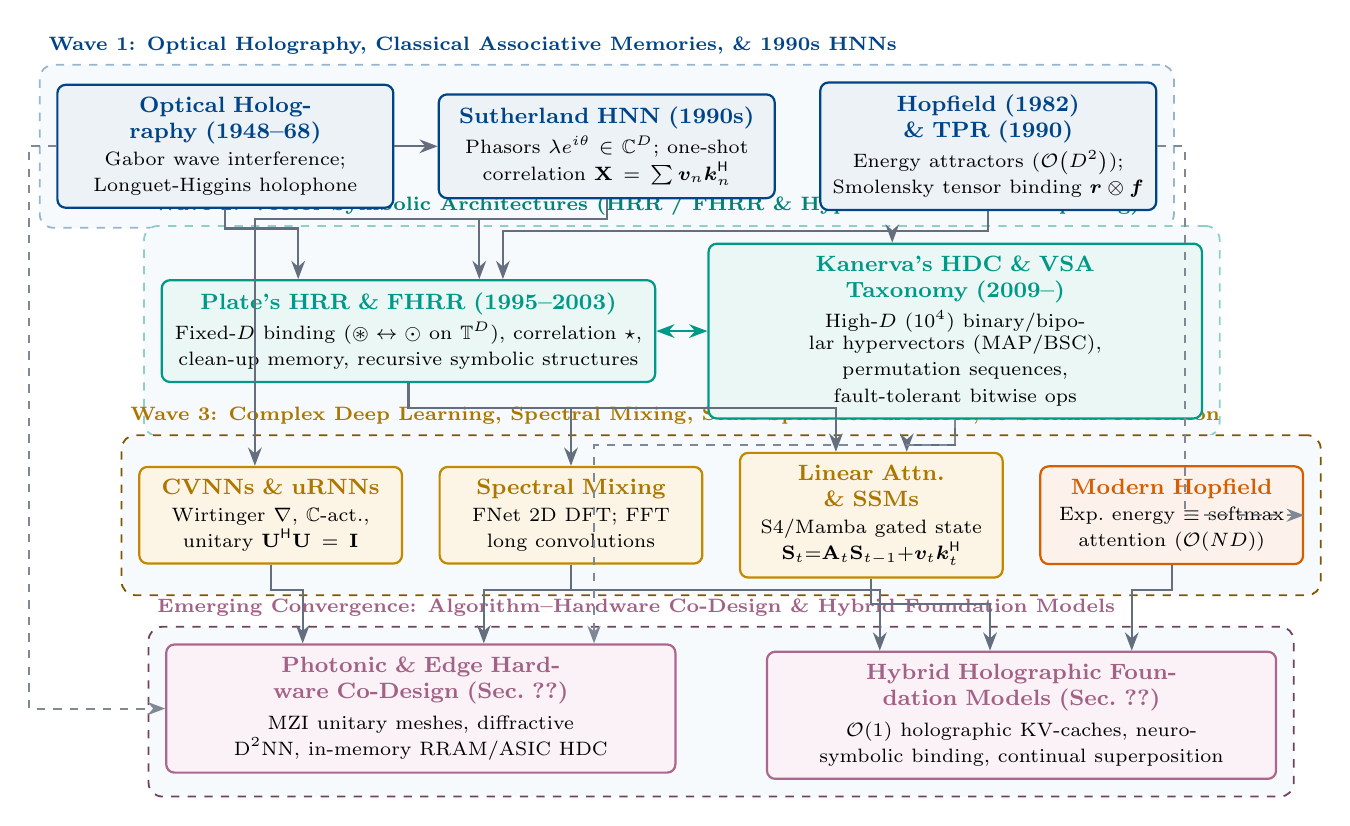
\begin{tikzpicture}[
    >=Stealth,
    node distance=0.85cm and 0.48cm,
    every node/.style={font=\footnotesize},
    gennode/.style={
        rectangle,
        rounded corners=3pt,
        line width=0.8pt,
        align=center,
        inner sep=4.5pt,
        minimum height=1.18cm
    },
    wave1/.style={
        gennode,
        draw=okabeNavy,
        fill=okabeNavy!7,
        text width=3.95cm
    },
    wave2/.style={
        gennode,
        draw=okabeTeal,
        fill=okabeTeal!8,
        text width=5.95cm
    },
    wave3/.style={
        gennode,
        draw=okabeAmber!85!black,
        fill=okabeAmber!10,
        text width=3.02cm
    },
    wave3alt/.style={
        gennode,
        draw=okabeCoral,
        fill=okabeCoral!8,
        text width=3.02cm
    },
    frontier/.style={
        gennode,
        draw=okabePurple!85!black,
        fill=okabePurple!10,
        text width=6.15cm
    },
    edgeflow/.style={
        ->,
        line width=0.8pt,
        draw=okabeSlate!85
    },
    crossflow/.style={
        ->,
        line width=0.75pt,
        dashed,
        draw=okabeSlate!70
    },
    eraband/.style={
        rounded corners=5pt,
        dashed,
        line width=0.65pt,
        inner sep=6pt
    }
]

% ==============================================================================
% TIER 1: FOUNDATIONS & WAVE 1 (1948 -- 1990s)
% ==============================================================================
\node[wave1] (sutherland) {%
    \textbf{\color{okabeNavy}Sutherland HNN (1990s)}\\[1.5pt]
    {\scriptsize Phasors $\lambda e^{i\theta} \in \C^D$; one-shot\\
    correlation $\mat{X}=\sum \vect{v}_n\vect{k}_n\herm$}%
};

\node[wave1, left=0.55cm of sutherland] (optics) {%
    \textbf{\color{okabeNavy}Optical Holography (1948--68)}\\[1.5pt]
    {\scriptsize Gabor wave interference;\\
    Longuet-Higgins holophone}%
};

\node[wave1, right=0.55cm of sutherland] (hopfield) {%
    \textbf{\color{okabeNavy}Hopfield (1982) \& TPR (1990)}\\[1.5pt]
    {\scriptsize Energy attractors ($\bigo{D^2}$);\\
    Smolensky tensor binding $\vect{r}\otimes\vect{f}$}%
};

% ==============================================================================
% TIER 2: WAVE 2 -- ALGEBRAIC VECTOR SYMBOLIC ARCHITECTURES (1995 -- 2010s)
% ==============================================================================
\coordinate (t1_left_mid) at ($(optics.south)!0.48!(sutherland.south)$);
\node[wave2, below=0.95cm of t1_left_mid] (hrr) {%
    \textbf{\color{okabeTeal}Plate's HRR \& FHRR (1995--2003)}\\[1.5pt]
    {\scriptsize Fixed-$D$ binding ($\cconv \leftrightarrow \hadamard$ on $\mathbb{T}^D$), correlation $\ccorr$,\\
    clean-up memory, recursive symbolic structures}%
};

\node[wave2, right=0.65cm of hrr] (hdc) {%
    \textbf{\color{okabeTeal}Kanerva's HDC \& VSA Taxonomy (2009--)}\\[1.5pt]
    {\scriptsize High-$D$ ($10^4$) binary/bipolar hypervectors (MAP/BSC),\\
    permutation sequences, fault-tolerant bitwise ops}%
};

% ==============================================================================
% TIER 3: WAVE 3 -- MODERN DEEP LEARNING CONVERGENCE (2016 -- PRESENT)
% ==============================================================================
\node[wave3, below=1.05cm of hrr, xshift=-1.75cm] (cvnn) {%
    \textbf{\color{okabeAmber!75!black}CVNNs \& uRNNs}\\[1.5pt]
    {\scriptsize Wirtinger $\nabla$, $\C$-act.,\\
    unitary $\mat{U}\herm\mat{U}=\mat{I}$}%
};

\node[wave3, right=0.45cm of cvnn] (spectral) {%
    \textbf{\color{okabeAmber!75!black}Spectral Mixing}\\[1.5pt]
    {\scriptsize FNet 2D DFT; FFT\\
    long convolutions}%
};

\node[wave3, right=0.45cm of spectral] (ssm) {%
    \textbf{\color{okabeAmber!75!black}Linear Attn.\ \& SSMs}\\[1.5pt]
    {\scriptsize S4/Mamba gated state\\
    $\mat{S}_t{=}\mat{A}_t\mat{S}_{t-1}{+}\vect{v}_t\vect{k}_t\herm$}%
};

\node[wave3alt, right=0.45cm of ssm] (modhop) {%
    \textbf{\color{okabeCoral}Modern Hopfield}\\[1.5pt]
    {\scriptsize Exp.\ energy $\equiv$ softmax\\
    attention ($\bigo{ND}$)}%
};

% ==============================================================================
% TIER 4: EMERGING FRONTIER (SECTIONS 5 -- 6)
% ==============================================================================
\coordinate (t3_left_mid) at ($(cvnn.south)!0.5!(spectral.south)$);
\node[frontier, below=1.0cm of t3_left_mid] (photonics) {%
    \textbf{\color{okabePurple!80!black}Photonic \& Edge Hardware Co-Design (Sec.~\ref{sec:applications})}\\[1.5pt]
    {\scriptsize MZI unitary meshes, diffractive $\text{D}^2\text{NN}$, in-memory RRAM/ASIC HDC}%
};

\coordinate (t3_right_mid) at ($(ssm.south)!0.5!(modhop.south)$);
\node[frontier, below=1.0cm of t3_right_mid] (hybrid) {%
    \textbf{\color{okabePurple!80!black}Hybrid Holographic Foundation Models (Sec.~\ref{sec:potentials})}\\[1.5pt]
    {\scriptsize $\bigo{1}$ holographic KV-caches, neuro-symbolic binding, continual superposition}%
};

% ==============================================================================
% DIRECTED LINEAGE EDGES
% ==============================================================================
% Tier 1 -> Tier 1 / Tier 2
\draw[edgeflow] (optics.east) -- (sutherland.west);
\draw[edgeflow] (optics.south) -- ++(0,-0.25) -| ([xshift=-1.4cm]hrr.north);
\draw[edgeflow] (sutherland.south) -- ++(0,-0.25) -| ([xshift=0.9cm]hrr.north);
\draw[edgeflow] (hopfield.south) -- ++(0,-0.25) -| ([xshift=1.2cm]hrr.north);
\draw[edgeflow] (hopfield.south) -- ++(0,-0.25) -| ([xshift=-0.8cm]hdc.north);

% Horizontal VSA synergy
\draw[<->, okabeTeal, line width=0.8pt] (hrr.east) -- (hdc.west);

% Tier 1/2 -> Tier 3
\draw[edgeflow] (sutherland.south) -- ++(0,-0.25) -| ([xshift=-0.2cm]cvnn.north);
\draw[edgeflow] (hrr.south) -- ++(0,-0.32) -| (spectral.north);
\draw[edgeflow] (hrr.south) -- ++(0,-0.32) -| ([xshift=-0.45cm]ssm.north);
\draw[edgeflow] (hdc.south) -- ++(0,-0.32) -| ([xshift=0.45cm]ssm.north);
\draw[crossflow] (hopfield.east) -- ++(0.35,0) |- (modhop.east);

% Tier 3 -> Tier 4
\draw[edgeflow] (cvnn.south) -- ++(0,-0.32) -| ([xshift=-1.5cm]photonics.north);
\draw[edgeflow] (spectral.south) -- ++(0,-0.32) -| ([xshift=0.8cm]photonics.north);
\draw[edgeflow] (spectral.south) -- ++(0,-0.32) -| ([xshift=-1.8cm]hybrid.north);
\draw[edgeflow] (ssm.south) -- ++(0,-0.32) -| ([xshift=-0.4cm]hybrid.north);
\draw[edgeflow] (modhop.south) -- ++(0,-0.32) -| ([xshift=1.4cm]hybrid.north);

% Direct optical & edge heritage into Tier 4 (routed cleanly outside left margin)
\draw[crossflow] (optics.west) -- ++(-0.35,0) |- (photonics.west);
\draw[crossflow] (hdc.south) -- ++(0,-0.32) -| ([xshift=2.2cm]photonics.north);

% ==============================================================================
% BACKGROUND ERA BANDS
% ==============================================================================
\begin{scope}[on background layer]
    \node[eraband, draw=okabeNavy!40, fill=okabeLightBg,
          fit=(optics)(sutherland)(hopfield),
          label={[anchor=south west, font=\scriptsize\bfseries, text=okabeNavy]north west:Wave 1: Optical Holography, Classical Associative Memories, \& 1990s HNNs}] {};
    \node[eraband, draw=okabeTeal!45, fill=okabeLightBg,
          fit=(hrr)(hdc),
          label={[anchor=south west, font=\scriptsize\bfseries, text=okabeTeal!85!black]north west:Wave 2: Vector Symbolic Architectures (HRR / FHRR \& Hyperdimensional Computing)}] {};
    \node[eraband, draw=okabeAmber!55!black, fill=okabeLightBg,
          fit=(cvnn)(spectral)(ssm)(modhop),
          label={[anchor=south west, font=\scriptsize\bfseries, text=okabeAmber!75!black]north west:Wave 3: Complex Deep Learning, Spectral Mixing, State-Space Recurrences, \& Softmax Attention}] {};
    \node[eraband, draw=okabePurple!55!black, fill=okabeLightBg,
          fit=(photonics)(hybrid),
          label={[anchor=south west, font=\scriptsize\bfseries, text=okabePurple!80!black]north west:Emerging Convergence: Algorithm--Hardware Co-Design \& Hybrid Foundation Models}] {};
\end{scope}

\end{tikzpicture}

    \caption{Historical and architectural genealogy of holographic neural computation. Solid arrows denote direct mathematical or algorithmic inheritance; dashed arrows highlight cross-era physical and architectural bridges linking optical holography to photonic accelerators (Section~\ref{sec:applications}) and classical Hopfield attractors to modern softmax attention (Section~\ref{sec:comparison}).}
    \label{fig:genealogy}
\end{figure}

% ------------------------------------------------------------------------------
\subsection{First Wave: Optical Analogies and 1990s Holographic Neural Networks}\label{sec:history:hnn}
% ------------------------------------------------------------------------------

\subsubsection{Optical and Associative Memory Precursors}

The conceptual genesis of holographic computation traces to Dennis Gabor's invention of optical holography~\cite{GABOR_1948_HOLOGRAPHY}, which demonstrated that a coherent wave field can record both the amplitude and relative phase of an object across an entire physical interference plate.
Because information is distributed globally across the interference pattern, illuminating even a fractured sub-region of the hologram with the original reference beam reconstructs the entire stored image with gracefully degraded resolution rather than localized erasure.
Two decades later, Longuet-Higgins translated this physical mechanism into a mathematical model of temporal associative recall---the \emph{holophone}~\cite{LONGUET_HIGGINS_1968_HOLOPHONE}---showing that linear correlation filters in the frequency domain could store and replay overlapping temporal sequences without dedicated memory slots.

In parallel, connectionist researchers developed matrix-based distributed associative memories, culminating in Hopfield's seminal energy-based attractor network~\cite{HOPFIELD_1982_ASSOCIATIVE}.
A classical Hopfield network stores $N$ bipolar patterns $\{\vect{\xi}_n\}_{n=1}^{N} \subset \{-1, +1\}^D$ inside a symmetric Hebbian outer-product weight matrix $\mat{W} = \frac{1}{D}\sum_{n=1}^{N} \vect{\xi}_n \vect{\xi}_n\trans$ and retrieves corrupted inputs via iterative sign updates minimizing $E(\vect{x}) = -\frac{1}{2}\vect{x}\trans \mat{W} \vect{x}$.
Although Hopfield networks are real-valued and auto-associative rather than complex phase-encoded, their outer-product superposition exhibits the exact crosstalk-limited linear capacity scaling ($N_{\max} \approx 0.138 D$ for uncorrelated patterns) that characterizes all bilinear holographic memories.

\subsubsection{Sutherland's Holographic Neural Network (HNN)}

In the early 1990s, John Sutherland synthesized optical phase interference with neural associative learning in the \emph{Holographic Neural Network (HNN)}~\cite{SUTHERLAND_1990_HNN}.
Rather than mapping scalar features through real-valued hidden layers trained by gradient descent, Sutherland's HNN embeds continuous real-valued stimulus vectors $\vect{s} \in \R^{D_s}$ directly onto the complex unit circle via a smooth sigmoidal phase transformation,
\begin{equation}\label{eq:sutherland_encoding}
    k_j = \lambda_j \exp\!\left(i \theta_j\right), \qquad
    \theta_j = 2\pi \sigma\!\left(\frac{s_j - \mu_j}{\tau_j}\right), \qquad
    \lambda_j \in [0, 1],
\end{equation}
where $\sigma(\cdot)$ denotes the logistic sigmoid (centering the empirical distribution of $s_j$ near zero phase to maximize angular spread across $[-\pi, \pi)$) and $\lambda_j$ encodes stimulus confidence.
Target responses $\vect{v} \in \C^{D_v}$ are phase-encoded analogously.

Sutherland's HNN enfolds a dataset of $N$ stimulus--response associations $\{(\vect{k}_n, \vect{v}_n)\}_{n=1}^N$ into a single complex correlation matrix $\mat{X} \in \C^{D_v \times D_k}$ via non-iterative (one-shot) Hebbian accumulation, $\mat{X} = \sum_{n=1}^{N} \vect{v}_n \vect{k}_n\herm$, as introduced in Remark~\ref{rem:sutherland_matrix}.
When real-world stimuli exhibit non-zero correlations ($\inner{\vect{k}_n}{\vect{k}_q} \neq 0$), one-shot enfolding accumulates systematic bias; Sutherland therefore introduced an iterative error-correcting \emph{enhanced learning} rule (a complex-valued Widrow--Hoff / Delta update),
\begin{equation}\label{eq:sutherland_delta}
    \mat{X}^{(t+1)} = \mat{X}^{(t)} + \eta_t\left(\vect{v}_n - \frac{1}{c_n}\mat{X}^{(t)}\vect{k}_n\right)\vect{k}_n\herm,
    \qquad c_n = \sum_{j=0}^{D_k - 1} \lambda_{n,j},
\end{equation}
which orthogonalizes interfering patterns across passes while remaining strictly local and linear in $\mat{X}$ (reducing at $\eta_0 = 1$, $\mat{X}^{(0)} = \mat{0}$ to one-shot accumulation $\mat{X} = \sum_n \vect{v}_n \vect{k}_n\herm$ with normalized recall $\hat{\vect{v}}_n = c_n^{-1}\mat{X}\vect{k}_n$ matching~\eqref{eq:sutherland_recall} on $\mathbb{T}^{D_k}$, or equivalently placing $c_n^{-1}$ outside the parentheses when $\mat{X}$ absorbs normalization for unnormalized readout $\mat{X}\vect{k}_n$).
To capture nonlinear decision boundaries without deep backpropagation, Sutherland further augmented the input vector with \emph{higher-order phase products}---explicitly constructing composite phasors $\prod_{r \in \mathcal{I}} \lambda_r e^{i\theta_r}$ for index subsets $\mathcal{I}$ of order $p \ge 2$---thereby lifting the stimulus into a higher-dimensional feature space $\C^{D'}$ ($D' \gg D_s$) where both nonlinear expressivity and superposition capacity scale with $D'$.

Despite demonstrating rapid one-shot learning, real-time control, and high fault tolerance in early industrial benchmarks, first-wave HNNs receded from mainstream machine learning during the late 1990s and 2000s.
Their reliance on hand-engineered polynomial phase expansions scaled combinatorially with raw sensory dimensionality, and unlike deep multilayer networks trained with stochastic gradient descent, shallow correlation matrices lacked a mechanism for learning hierarchical, invariant feature representations from raw pixels or natural language.

% ------------------------------------------------------------------------------
\subsection{Second Wave: Vector Symbolic Architectures (HRR and HDC)}\label{sec:history:vsa}
% ------------------------------------------------------------------------------

While Sutherland targeted continuous-valued associative mapping, a parallel community in cognitive science and symbolic AI confronted the \emph{binding problem}: how distributed neural vectors can represent structured, compositional objects---such as nested trees, predicate--argument tuples, and variable bindings---without suffering the superposition catastrophe (conflating ``red square + blue circle'' with ``red circle + blue square'').

\subsubsection{From Tensor Products to Plate's Holographic Reduced Representations}

Paul Smolensky first showed that variable binding in connectionist spaces can be realized cleanly via \emph{Tensor Product Representations (TPRs)}~\cite{SMOLENSKY_1990_TPR}, representing a set of role--filler bindings as $\mat{T} = \sum_{n=1}^{N} \vect{r}_n \otimes \vect{f}_n \in \R^{D \times D}$.
However, recursively binding a composite structure to a higher-level role increases tensor rank at every level of nesting, causing storage complexity to explode exponentially as $\bigo{D^r}$ for depth-$r$ trees.

Tony Plate resolved this dimensionality explosion in 1995 with \emph{Holographic Reduced Representations (HRRs)}~\cite{PLATE_1995_HRR}.
Plate observed that circular convolution $\vect{r} \cconv \vect{f} \in \R^D$ is precisely the \emph{compressed anti-diagonal projection} of the unconjugated outer-product tensor $\vect{r} \otimes \vect{f}$: summing entries $(a,b)$ along wrapped anti-diagonals $(a + b) \bmod D = j$ collapses a rank-2 tensor back into $\R^D$ (whereas summing along wrapped main diagonals $(a - b) \bmod D = j$, as on the Hermitian correlation matrix~\eqref{eq:hnn_corr_matrix}, yields circular correlation $\vect{k} \ccorr \vect{v} = \inv{\vect{k}} \cconv \vect{v}$).
Because the output resides in the exact same ambient space as its operands, HRRs permit arbitrary recursive nesting at constant width $D$: for example, a structured proposition $\texttt{eat}(\texttt{agent}{=}\texttt{dog}, \texttt{object}{=}\texttt{bone})$ can be encoded recursively as
\begin{equation}\label{eq:hrr_recursive}
    \vect{p} = \vect{r}_{\mathrm{pred}} \cconv \vect{f}_{\mathrm{eat}}
             + \vect{r}_{\mathrm{agent}} \cconv \vect{f}_{\mathrm{dog}}
             + \vect{r}_{\mathrm{obj}} \cconv \vect{f}_{\mathrm{bone}} \in \R^D,
\end{equation}
and subsequently bound as a filler inside an outer sentence vector without expanding dimensionality.
Plate further formalized the clean-up memory required to strip crosstalk noise after circular-correlation unbinding ($\ccorr$), proved the foundational variance bounds analyzed in Section~\ref{sec:math:capacity}, and introduced complex-valued \emph{Fourier HRR (FHRR)} on $\mathbb{T}^D$ to eliminate spectral self-distortion and accelerate binding to $\bigo{D}$ elementwise phase addition.
More recently, Generalized HRRs (GHRRs)~\cite{YEUNG_2024_GHRR} lifted scalar FHRR phasors in $\mathbb{T}^D$ to $m \times m$ unitary matrix elements in $U(m)^D$, enabling natively non-commutative binding and flexible similarity kernels while recovering standard FHRR at $m=1$.
Bridging these second-wave algebras directly into deep sequence modeling, Alam et al.~\cite{HOLOGRAPHIC_ATTENTION_OR_KV_CACHE} recast Transformer self-attention via compressive HRR binding and unbinding to reduce attention complexity to linear-in-$N$ superposition traces.

\subsubsection{Kanerva's Hyperdimensional Computing and VSA Unification}

Building on sparse distributed memory and random-projection geometry, Pentti Kanerva articulated \emph{Hyperdimensional Computing (HDC)}~\cite{KANERVA_2009_HDC}, emphasizing ultra-high-dimensional ($D \sim 10^4$) random binary or bipolar \emph{hypervectors} ($\{0, 1\}^D$ or $\{-1, +1\}^D$).
In addition to elementwise binding ($\hadamard$ or XOR) and majority-vote/additive bundling, Kanerva highlighted a third primitive---invertible coordinate \emph{permutation} $\rho: \R^D \to \R^D$ (typically a cyclic shift)---to break the commutativity of binding and encode ordered sequences, $n$-grams, and temporal trajectories:
\begin{equation}\label{eq:hdc_sequence}
    \vect{s}_{1:L} = \sum_{t=1}^{L} \rho^{L - t}\!\left(\vect{x}_t\right)
    \qquad\text{or}\qquad
    \vect{g}_{1:L} = \bigodot_{t=1}^{L} \rho^{L - t}\!\left(\vect{x}_t\right).
\end{equation}
Kanerva demonstrated that holistic algebraic analogies (such as solving ``What is the Dollar of Mexico?'' by unbinding $\vect{k}_{\mathrm{USA}}$ and rebinding $\vect{k}_{\mathrm{Mexico}}$ across bundled country records) execute in a single constant-time parallel vector operation without explicit symbolic search trees.

Subsequent surveys by Schlegel et al.~\cite{SCHLEGEL_VSA_COMPARISON} and Kleyko et al.~\cite{KLEYKO_VSA_SURVEY} unified HRR, FHRR, HDC, Multiply--Add--Permute (MAP), Binary Spatter Codes (BSC), and Sparse Binary Distributed Representations under the umbrella term \emph{Vector Symbolic Architectures (VSAs)}.
Across this taxonomy, every VSA is uniquely characterized by four design choices: (1) ambient vector space and atomic distribution ($\{0,1\}^D$, $\{-1,+1\}^D$, $\R^D$, or $\mathbb{T}^D$); (2) binding algebra and whether unbinding is exact (e.g., XOR, MAP, FHRR) or approximate (real Gaussian HRR); (3) bundling linearity vs.\ clipping/phase-projection; and (4) clean-up mechanism (linear codebook matching, Hopfield attractors, or multi-factor resonator networks).

% ------------------------------------------------------------------------------
\subsection{Third Wave: Spectral Mixing, Complex Deep Learning, and State-Space Models}\label{sec:history:modern}
% ------------------------------------------------------------------------------

Over the past decade, deep learning architectures designed for scalability and long-sequence stability have independently rediscovered---and scaled via end-to-end backpropagation---each core mathematical ingredient of holographic computation.

\subsubsection{Complex-Valued Neural Networks (CVNNs) and Unitary Recurrences}

Modern Complex-Valued Neural Networks~\cite{BASSEY_CVNN_SURVEY,TRABELSI_2018_DCN} extend deep convolutional, residual, and attention layers natively into $\C^D$.
Because Liouville's theorem prohibits non-constant bounded holomorphic activations on $\C$, CVNNs rely on \emph{Wirtinger ($\C\R$) calculus} to optimize real-valued objective functions $\mathcal{L}(\vect{z}, \conj{\vect{z}}) \in \R$ with respect to complex weights $\vect{z} = \vect{x} + i\vect{y}$ via the conjugate gradient
\begin{equation}\label{eq:wirtinger}
    \nabla_{\conj{\vect{z}}} \mathcal{L}
    \coloneqq \frac{\partial \mathcal{L}}{\partial \conj{\vect{z}}}
    = \frac{1}{2}\left(\frac{\partial \mathcal{L}}{\partial \vect{x}} + i\frac{\partial \mathcal{L}}{\partial \vect{y}}\right),
\end{equation}
paired with split or phase-preserving nonlinearities such as $\C$ReLU (applying ReLU separately to real and imaginary parts) and $\mathrm{modReLU}(z) = \mathrm{ReLU}(\abs{z} + b)\frac{z}{\abs{z}}$ (which preserves phase angle $\theta$ identically while gating magnitude $\lambda$).
Closely aligned with unitary holographic binding, \emph{Unitary Evolution Recurrent Neural Networks (uRNNs)}~\cite{ARJOVSKY_2016_URNN} parameterize recurrent transitions as products of complex diagonal phase matrices, FFT/IFFT blocks, and Householder reflections so that $\mat{U}\herm \mat{U} = \mat{I}_D$.
Because unitary operators preserve Euclidean norm exactly ($\norm{\mat{U}\vect{h}}_2 = \norm{\vect{h}}_2$), uRNNs eliminate exploding and vanishing gradients over long horizons purely through complex phase interference---bridging Sutherland's phase-space formulation with deep recurrent optimization.

\subsubsection{Fourier Token Mixing and Spectral Convolutions}

A second point of convergence emerged in efforts to replace quadratic $\bigo{N^2}$ Transformer self-attention~\cite{VASWANI_TRANSFORMER} with sub-quadratic spectral mixing.
FNet~\cite{LEE_THORP_FNET} replaces the multi-head self-attention sublayer entirely with an unparameterized two-dimensional Discrete Fourier Transform across the sequence and hidden dimensions,
\begin{equation}\label{eq:fnet}
    \mat{Y} = \Real\!\left(\DFT_{\mathrm{seq}}\!\left(\DFT_{\mathrm{hidden}}(\mat{H})\right)\right),
\end{equation}
achieving $\bigo{N \log N}$ token mixing while retaining competitive downstream accuracy on natural-language benchmarks at a fraction of the computational cost.
Subsequent global-filter and FFT long-convolution models generalize~\eqref{eq:fnet} by introducing learnable frequency-domain filters $\vect{W}_\omega \in \C^D$, computing $\IDFT(\vect{W} \hadamard \DFT(\vect{x}))$ across sequence positions.
By the Circular Convolution Theorem (Proposition~\ref{prop:conv_thm}), every such spectral mixing layer is algebraically equivalent to circular-convolution holographic binding between input representations and a learned kernel, executed in $\bigo{N \log N}$ time via FFT.

\subsubsection{Linear Attention, State-Space Models, and Modern Hopfield Networks}

Most remarkably, modern sub-quadratic sequence models have converged directly onto the exact mathematical form of holographic associative superposition.
Katharopoulos et al.~\cite{KATHAROPOULOS_2020_LINEAR_TRANSFORMER} showed that replacing the exponential softmax kernel in Transformer attention with a separable positive feature map $\phi(\cdot)$ rewrites causal attention as a recurrent fixed-size associative matrix,
\begin{equation}\label{eq:linear_attn_state}
    \mat{S}_t = \mat{S}_{t-1} + \vect{v}_t \phi(\vect{k}_t)\trans,
    \qquad
    \hat{\vect{v}}_t = \frac{\mat{S}_t \phi(\vect{q}_t)}{\vect{z}_t\trans \phi(\vect{q}_t)},
\end{equation}
where $\vect{z}_t = \sum_{\tau=1}^{t} \phi(\vect{k}_\tau)$ normalizes the readout.
Comparing~\eqref{eq:linear_attn_state} with Sutherland's complex correlation matrix~\eqref{eq:sutherland_recall} reveals an exact structural isomorphism: linear attention is a real-valued, end-to-end learned holographic outer-product memory whose fixed state size $\bigo{D^2}$ suffers precisely from the crosstalk saturation analyzed in Section~\ref{sec:math:capacity}.

Structured and Selective State-Space Models (S4 and Mamba)~\cite{GU_SSM_S4_MAMBA} resolve the static saturation of unbounded additive traces by introducing continuous-time (frequently complex-diagonalized) dynamics and input-dependent forgetting gates:
\begin{equation}\label{eq:ssm_recurrence}
    \mat{S}_t = \mat{A}_t \mat{S}_{t-1} + \vect{B}_t \vect{x}_t,
    \qquad
    \vect{y}_t = \mat{C}_t \mat{S}_t,
\end{equation}
where $\mat{A}_t$ selectively decays stale superposed bindings to preserve $\SNR$ for salient recent or key-matched information---the continuous, learned counterpart to weighted holographic bundling~\eqref{eq:bundling} and Sutherland's delta-rule interference suppression~\eqref{eq:sutherland_delta}.
Extending this matrix-state lineage, DeltaNet~\cite{YANG_2024_DELTANET} and Gated DeltaNet~\cite{YANG_2025_GATED_DELTANET} scale Sutherland's error-correcting delta rule~\eqref{eq:sutherland_delta} into chunkwise hardware-efficient linear Transformers, combining rank-one key--value erasure with selective decay to actively suppress cross-key interference.
In parallel, frontier hybrid models---exemplified by Griffin~\cite{DE_2024_GRIFFIN} (interleaving gated linear recurrences with local sliding-window attention) and Titans~\cite{BEHROUZ_2025_TITANS} (pairing local exact attention with a deep neural long-term memory updated at test time via surprise-driven gradient descent)---operationalize the exact division of labor between fixed-state compression and exact local recall.
In stark contrast to this fixed-size parametric superposition lineage, Ramsauer et al.~\cite{RAMSAUER_MODERN_HOPFIELD} proved that lifting Hopfield's classical quadratic energy to a continuous log-sum-exp energy yields an associative memory with \emph{exponential} pattern storage capacity whose single-step update is mathematically identical to Transformer scaled dot-product softmax attention~\cite{VASWANI_TRANSFORMER}---at the unavoidable cost of retaining every stored pattern explicitly in $\bigo{ND}$ memory.

% ------------------------------------------------------------------------------
\subsection{Unifying Architectural Perspective}\label{sec:history:synthesis}
% ------------------------------------------------------------------------------

Viewing all three waves through the mathematical lens of Section~\ref{sec:math} exposes a clean architectural bifurcation across modern AI:
\begin{itemize}
    \item \emph{Parametric holographic superposition} (Sutherland HNNs, HRR/FHRR, HDC, linear attention, and SSMs) compresses unbounded histories into a constant-size latent state ($\bigo{D}$ for vector binding or $\bigo{D^2}$ for outer-product matrices), delivering $\bigo{1}$ per-step inference memory and native phase/hardware affinity at the cost of additive crosstalk governed by $\SNR \propto D/N$.
    \item \emph{Non-parametric explicit attention} (Modern Hopfield Networks and softmax Transformers) avoids crosstalk by retaining all $N$ keys and values explicitly ($\bigo{ND}$ memory and $\bigo{N^2}$ pairwise interaction), enabling exact verbatim recall at severe long-context memory and energy overhead.
\end{itemize}
This dichotomy forms the analytical foundation for the systematic multi-axis comparison in Section~\ref{sec:comparison} and motivates the hybrid holographic--attention architectures examined in Section~\ref{sec:potentials}.

\section{Comparative Analysis of Memory and Attention Paradigms}\label{sec:comparison}

Having established the algebraic foundations of phase-space superposition and traced the historical lineage from optical holography and Sutherland's Holographic Neural Networks (HNNs) through Vector Symbolic Architectures (VSAs) to contemporary Complex-Valued Neural Networks (CVNNs), Fourier mixing, and State-Space Models (SSMs), we now situate holographic representations within the broader landscape of neural associative memory and sequence-modeling architectures.
A persistent obstacle to cross-pollination between the VSA/HNN community and mainstream deep learning has been the lack of a unified analytical vocabulary: mechanisms that appear distinct at the implementation level---such as complex correlation matrices, circular-convolution memory traces, Hopfield energy landscapes, and Transformer key--value caches---often represent different operating points along a single mathematical trade-off between \emph{parametric compression} and \emph{non-parametric retention}.
In this section, we define six rigorous evaluation axes, synthesize a cross-paradigm taxonomy (Table~\ref{tab:paradigm_comparison}), formalize where linear attention and SSMs interpolate between holographic superposition and dense attention, and characterize the capacity--expressivity--compute trade-offs that govern when each paradigm excels.

\subsection{Evaluation Axes and Analytical Framework}\label{sec:comparison:axes}

To compare representational paradigms on an equal footing, let $N$ denote the number of stored key--value associations (or active context tokens in an autoregressive sequence) and $D$ denote the ambient representation dimension (e.g., hypervector width, complex phasor dimension, or model hidden width).
We benchmark each architectural family along six orthogonal dimensions:

\paragraph{1.\ Memory Footprint and State Complexity.}
We distinguish persistent memory state required to store $N$ items from transient working activations.
Fixed-state parametric memories compress an arbitrary stream of $N$ associations into a constant-size vector trace $\vect{m} \in \C^D$ ($\bigo{D}$ space, i.e., $\bigo{1}$ growth in $N$) or a fixed correlation matrix $\mat{X} \in \C^{D \times D}$ ($\bigo{D^2}$ space, likewise $\bigo{1}$ in $N$).
Conversely, non-parametric associative architectures retain every historical key--value pair explicitly in a growing cache of size $\bigo{ND}$, and dense full-sequence self-attention additionally materializes $\bigo{N^2}$ pairwise interaction scores unless tiled via hardware-aware fused kernels.

\paragraph{2.\ Retrieval and Inference Complexity.}
Given a query cue $\vect{k}$, we measure the per-query arithmetic complexity and memory-bandwidth demand required to retrieve the associated value $\hat{\vect{v}}$.
Holographic vector unbinding executes in $\bigo{D}$ elementwise operations in the frequency domain (via conjugate Hadamard modulation $\hadamard$) or bipolar space (via bitwise XOR), and in $\bigo{D \log D}$ via the Fast Fourier Transform (FFT) for time-domain circular correlation $\ccorr$.
Matrix correlation memories require $\bigo{D^2}$ multiply--accumulate operations per query, whereas autoregressive attention over an explicit cache incurs $\bigo{ND}$ compute and $\bigo{ND}$ memory bandwidth per generated token---creating the well-known memory-bound decoding bottleneck at large $N$.

\paragraph{3.\ Training, Update, and Plasticity Paradigm.}
Paradigms diverge sharply in how associations are acquired and revised.
Algebraic VSA/HDC encoders and classical Hebbian/correlation HNNs support \emph{one-shot} online insertion ($\vect{m}_{t} = \vect{m}_{t-1} + \vect{k}_t \cconv \vect{v}_t$) and approximate deletion ($\vect{m}_{t} - \vect{k}_j \cconv \vect{v}_j$) without gradient descent, making them naturally suited to continual or resource-constrained adaptation.
In contrast, Transformer attention and modern deep architectures rely on iterative end-to-end backpropagation to learn rich projection geometry, while hybrid architectures combine gradient-trained neural encoders with algebraic holographic memory modules.

\paragraph{4.\ Symbolic Compositionality and Variable Binding.}
We assess whether a paradigm natively supports dimension-preserving \emph{role--filler binding} and recursive structural composition.
In tensor-product representations~\cite{SMOLENSKY_1990_TPR}, binding $k$ symbols produces a rank-$k$ tensor of size $D^k$, causing exponential dimensionality explosion.
VSAs and HNNs resolve this via compressed binding ($\cconv$ or $\hadamard$), mapping $\C^D \times \C^D \to \C^D$ so that arbitrarily nested trees, graphs, and key--value records inhabit the same ambient space $\C^D$ and remain algebraically queryable.
By contrast, classical Hopfield networks act primarily as flat pattern-completion attractors, and standard Transformers achieve compositional reasoning implicitly through multi-layer attention routing rather than explicit algebraic variable binding.

\paragraph{5.\ Noise Tolerance, Capacity Scaling, and Degradation Profile.}
Beyond peak storage capacity $N_{\max}(D)$, the \emph{geometry of failure} matters critically in real systems.
Holographic superposition degrades smoothly and predictably as load $N/D$ increases: additive crosstalk noise $\vect{\eta}$ scales continuously such that $\SNR \propto D/N$, and distributed encoding confers intrinsic resilience to coordinate erasures, quantization, and hardware bit-flips~\cite{FRADY_CAPACITY_VSA,KLEYKO_VSA_SURVEY}.
Classical binary Hopfield networks exhibit attractor-basin error correction up to a sharp spin-glass phase transition at critical load $\alpha_c = N_{\max}/D \approx 0.138$, beyond which retrieval collapses catastrophically~\cite{HOPFIELD_1982_ASSOCIATIVE,AMIT_1985_HOPFIELD_CAPACITY}.
Modern continuous Hopfield networks and softmax attention suppress crosstalk exponentially, achieving exponential pattern capacity in $D$ under bounded separation margins~\cite{RAMSAUER_MODERN_HOPFIELD}, yet remain sensitive to out-of-distribution attention dilution and aggressive low-bitweight quantization.

\paragraph{6.\ Hardware Affinity and Physical Execution Model.}
Finally, we evaluate alignment with computational substrates.
Dense Transformers are co-optimized for GPU/TPU systolic arrays executing high-arithmetic-intensity general matrix multiplications (GEMMs).
Binary/bipolar HDC maps directly onto bitwise SIMD pipelines, low-power FPGAs, microcontrollers, and analog resistive crossbars~\cite{RAHIMI_HDC_EDGE,KARUNARATNE_2020_PCM_HDC}.
Complex-phasor HNNs and Fourier-domain HRRs exhibit a unique physical isomorphism with coherent photonic interferometers and diffractive optical processors, where wave interference and lens-based Fourier transforms execute passively at optical bandwidth~\cite{SHEN_PHOTONIC_MZI,LIN_DIFFRACTIVE_OPTICAL_NN}.

\subsection{Systematic Cross-Paradigm Comparison}\label{sec:comparison:table}

Table~\ref{tab:paradigm_comparison} summarizes the four foundational paradigms---Classical HNNs~\cite{SUTHERLAND_1990_HNN}, HRR/HDC (VSAs)~\cite{PLATE_1995_HRR,KANERVA_2009_HDC,SCHLEGEL_VSA_COMPARISON}, Classical and Modern Hopfield Networks~\cite{HOPFIELD_1982_ASSOCIATIVE,RAMSAUER_MODERN_HOPFIELD}, and Transformer Self-Attention~\cite{VASWANI_TRANSFORMER}---across the evaluation axes defined above.
Below, we dissect the structural relationships connecting these families and clarify how modern Linear Attention~\cite{KATHAROPOULOS_2020_LINEAR_TRANSFORMER} and State-Space Models~\cite{GU_SSM_S4_MAMBA} bridge the divide between parametric superposition and non-parametric attention.

\begin{table}[htbp]
\centering
\caption{Systematic Comparative Taxonomy of Holographic, Vector-Symbolic, Associative, and Attention Paradigms. Here $N$ denotes the number of stored associations or context tokens, $D$ denotes the ambient state or hidden dimension, and $M$ denotes the cleanup codebook cardinality.}
\label{tab:paradigm_comparison}
\scriptsize
\setlength{\tabcolsep}{4pt}
\renewcommand{\arraystretch}{1.24}
\begin{tabularx}{\textwidth}{@{} >{\raggedright\arraybackslash}p{2.35cm} >{\raggedright\arraybackslash}X >{\raggedright\arraybackslash}X >{\raggedright\arraybackslash}X >{\raggedright\arraybackslash}X @{}}
\toprule
\textbf{Criterion} & \textbf{Classical HNN}~\cite{SUTHERLAND_1990_HNN} & \textbf{HRR / HDC (VSA)}~\cite{PLATE_1995_HRR,KANERVA_2009_HDC} & \textbf{Hopfield (Classic / Modern)}~\cite{HOPFIELD_1982_ASSOCIATIVE,RAMSAUER_MODERN_HOPFIELD} & \textbf{Transformer Attention}~\cite{VASWANI_TRANSFORMER} \\
\midrule
State Space \& Encoding & Complex phasors $\C^D$ (unit-magnitude or weighted phase) & $\R^D$, $\C^D$ (FHRR), or $\{-1,+1\}^D$ / $\{0,1\}^D$ & $\{-1,+1\}^D$ (classic) / continuous $\R^D$ (modern) & Continuous real latent vectors $\R^D$ \\
\addlinespace[2pt]
Memory Footprint & $\bigo{D^2}$ correlation matrix (or $\bigo{D}$ per output); $\bigo{1}$ in $N$ & $\bigo{D}$ single trace vector; $\bigo{1}$ in $N$ & $\bigo{D^2}$ (classic) / $\bigo{ND}$ explicit pattern matrix (modern) & $\bigo{ND}$ KV-cache; $\bigo{N^2}$ dense score matrix \\
\addlinespace[2pt]
Per-Query Retrieval Compute & $\bigo{D^2}$ complex matrix--vector correlation & $\bigo{D}$ ($\hadamard$/XOR) or $\bigo{D\log D}$ (FFT $\ccorr$) & $\bigo{D^2}$ per step (classic) / $\bigo{ND}$ softmax step (modern) & $\bigo{ND}$ autoregressive; $\bigo{N^2 D}$ full sequence \\
\addlinespace[2pt]
Binding / Retrieval Mechanism & Complex Hermitian correlation $\mat{X}\vect{k}$ and phase folding & Binding $\cconv$ / $\hadamard$ / XOR; unbinding $\ccorr$ / $\conj{\vect{k}}\hadamard\vect{m}$ & Energy descent (classic) / $\mat{K}\trans\operatorname{softmax}(\beta\mat{K}\vect{q})$ & Scaled dot-product $\mat{V}\trans\operatorname{softmax}(\mat{K}\vect{q}/\sqrt{d_k})$ \\
\addlinespace[2pt]
Storage Capacity ($N_{\max}$) & $\bigo{D}$ per output channel (crosstalk-limited) & $\bigo{D / \log M}$ with cleanup codebook~\cite{FRADY_CAPACITY_VSA} & $\approx 0.138D$ (classic)~\cite{AMIT_1985_HOPFIELD_CAPACITY} / $\bigo{c^{D/2}}$ (modern) & Unbounded in $D$ up to cache size $N$; sharp softmax separation \\
\addlinespace[2pt]
Training \& Update Paradigm & One-shot correlation / iterative phase-error folding & Training-free algebraic / single-pass / hybrid SGD & Hebbian outer product / differentiable energy network & End-to-end iterative backpropagation (SGD/Adam) \\
\addlinespace[2pt]
Symbolic Compositionality & Moderate (higher-order phase products) & High (native dimension-preserving role--filler nesting) & Low (flat auto-associative pattern completion) & Implicit / emergent via deep multi-head routing \\
\addlinespace[2pt]
Noise \& Fault Tolerance & High (graceful $\SNR \propto D/N$ decay) & Very high (blessing of dimensionality; BER-resilient) & High within attractor basins; sharp collapse past $\alpha_c$ (classic) & Moderate (sensitive to quantization and attention dilution) \\
\addlinespace[2pt]
Primary Hardware Affinity & Coherent photonics / phase-domain optics & Edge MCU / FPGA / ASIC / analog IMC crossbars & Analog crossbars (classic) / GPU tensor cores (modern) & GPU / TPU dense GEMM accelerators \\
\bottomrule
\end{tabularx}
\end{table}

\paragraph{Classical HNNs versus HRR/HDC: Matrix Correlation vs.\ Vector Folding.}
Both Sutherland's HNN~\cite{SUTHERLAND_1990_HNN} and Plate's HRR~\cite{PLATE_1995_HRR} encode stimulus--response pairs $\{(\vect{k}_n, \vect{v}_n)\}_{n=1}^N$ via distributed phase interference, yet they differ crucially in spatial compression.
A classical HNN maintains a complex Hermitian correlation matrix
\begin{equation}\label{eq:hnn_corr_matrix}
    \mat{X} = \sum_{n=1}^{N} \vect{v}_n \vect{k}_n\herm \in \C^{D \times D},
\end{equation}
so that querying with $\vect{k}_q$ yields $\hat{\vect{v}}_q = \frac{1}{D}\mat{X}\vect{k}_q = \vect{v}_q + \frac{1}{D}\sum_{n \neq q} (\vect{k}_n\herm\vect{k}_q)\vect{v}_n$ (for unit-modulus phasor keys satisfying $\vect{k}_n\herm\vect{k}_n = D$).
In contrast, HRR and Fourier HRR (FHRR) fold the rank-$N$ outer-product superposition into a single $\bigo{D}$ trace vector: consistent with Section~\ref{sec:history:vsa}, summing the unconjugated outer products $\sum_{n=1}^{N} \vect{k}_n \otimes \vect{v}_n$ along wrapped anti-diagonals $(a + b) \bmod D = j$ yields the circular-convolution trace $\vect{m} = \sum_{n=1}^N \vect{k}_n \cconv \vect{v}_n$ (or $\DFT\{\vect{m}\} = \sum_{n=1}^N \DFT\{\vect{k}_n\} \hadamard \DFT\{\vect{v}_n\}$ in the frequency domain), whereas summing the Hermitian correlation matrix $\mat{X}$ in~\eqref{eq:hnn_corr_matrix} along wrapped main diagonals $(a - b) \bmod D = j$ yields the circular-correlation trace $\sum_{n=1}^N \vect{k}_n \ccorr \vect{v}_n$.
Because each coordinate of $\vect{m}$ aggregates $D$ pairwise outer-product entries, HRR/HDC slashes memory complexity from $\bigo{D^2}$ to $\bigo{D}$ and retrieval compute from $\bigo{D^2}$ to $\bigo{D \log D}$ (or $\bigo{D}$ in phase space), while preserving identical $\bigo{D}$ asymptotic capacity scaling per trace---at the cost of a modest constant-factor increase in crosstalk variance that is readily suppressed by a downstream cleanup memory~\cite{PLATE_1995_HRR,SCHLEGEL_VSA_COMPARISON}.

\paragraph{From Classical Hopfield Networks to Modern Hopfield and Transformer Attention.}
The classical Hopfield network~\cite{HOPFIELD_1982_ASSOCIATIVE} constructs a symmetric real auto-associative matrix $\mat{W} = \frac{1}{D}\sum_{n=1}^N \vect{x}_n \vect{x}_n\trans \in \R^{D \times D}$, which is structurally a real, bipolar, unkeyed special case of~\eqref{eq:hnn_corr_matrix}.
Because its quadratic energy $E(\vect{q}) = -\frac{1}{2}\vect{q}\trans\mat{W}\vect{q}$ relies on linear inner-product superposition, cross-terms $\sum_{n \neq q} (\vect{x}_n\trans \vect{q})\vect{x}_n$ accumulate linearly with $N$, imposing the strict spin-glass capacity ceiling $N_{\max} \approx 0.138 D$~\cite{AMIT_1985_HOPFIELD_CAPACITY}.
Modern continuous Hopfield networks~\cite{RAMSAUER_MODERN_HOPFIELD} shatter this linear barrier by replacing the quadratic interaction with a log-sum-exp energy over an \emph{explicitly stored} matrix of patterns $\mat{K} = [\vect{k}_1, \dots, \vect{k}_N]\trans \in \R^{N \times D}$:
\begin{equation}\label{eq:modern_hopfield_energy}
    E(\vect{q}) = -\beta^{-1}\log\!\left(\sum_{n=1}^{N} \exp\!\left(\beta\,\vect{k}_n\trans\vect{q}\right)\right) + \frac{1}{2}\norm{\vect{q}}_2^2 + \text{const.},
\end{equation}
where $\beta > 0$ is an inverse temperature.
Minimizing~\eqref{eq:modern_hopfield_energy} via the concave--convex procedure yields the single-step retrieval rule
\begin{equation}\label{eq:modern_hopfield_update}
    \vect{q}^{\text{new}} = \mat{K}\trans \operatorname{softmax}\!\left(\beta \mat{K}\vect{q}\right).
\end{equation}
Decoupling the stored keys $\mat{K} \in \R^{N \times d_k}$ from associated values $\mat{V} \in \R^{N \times d_v}$ and setting $\beta = 1/\sqrt{d_k}$ recovers the exact scaled dot-product attention head of the Transformer~\cite{VASWANI_TRANSFORMER}:
\begin{equation}\label{eq:transformer_attn}
    \operatorname{Attn}(\vect{q}, \mat{K}, \mat{V}) = \mat{V}\trans \operatorname{softmax}\!\left(\frac{\mat{K}\vect{q}}{\sqrt{d_k}}\right).
\end{equation}
This equivalence illuminates the core trade-off in Table~\ref{tab:paradigm_comparison}: the exponential kernel inside $\operatorname{softmax}(\cdot)$ exponentially dampens non-matching inner products, eliminating additive holographic crosstalk $\vect{\eta}$ and elevating theoretical capacity from $\bigo{D}$ to exponential in $D$.
However, that exponential nonlinearity cannot be factored across the summation over $n$, forcing the model to abandon fixed-size superposition and retain all $N$ keys and values explicitly at $\bigo{ND}$ memory cost.

\paragraph{Where Linear Attention and State-Space Models Interpolate.}
Applying the epistemic taxonomy of Section~\ref{sec:intro:methodology}, contemporary sub-quadratic sequence models connect to~\eqref{eq:hnn_corr_matrix} and~\eqref{eq:transformer_attn} across distinct levels of mathematical rigor.
In kernelized Linear Attention~\cite{KATHAROPOULOS_2020_LINEAR_TRANSFORMER}, the unfactorable exponential similarity $\exp(\vect{k}_n\trans\vect{q}/\sqrt{d_k})$ is approximated by an explicit feature-map inner product $\phi(\vect{k}_n)\trans\phi(\vect{q})$ with $\phi: \R^{d_k} \to \R^{D_\phi}$.
Applying associativity of matrix multiplication collapses the $\bigo{ND}$ cache back into a fixed-size recurrent correlation state:
\begin{equation}\label{eq:comp_linear_attn_state}
    \mat{S}_t = \mat{S}_{t-1} + \vect{v}_t \phi(\vect{k}_t)\trans = \sum_{\tau=1}^{t} \vect{v}_\tau \phi(\vect{k}_\tau)\trans \in \R^{d_v \times D_\phi},
    \qquad
    \hat{\vect{v}}_t = \frac{\mat{S}_t \phi(\vect{q}_t)}{\vect{z}_t\trans \phi(\vect{q}_t)},
\end{equation}
where $\vect{z}_t = \sum_{\tau=1}^t \phi(\vect{k}_\tau)$.
Comparing~\eqref{eq:comp_linear_attn_state} directly with~\eqref{eq:hnn_corr_matrix} yields an \emph{exact algebraic equivalence} (up to real-field restriction and scalar denominator normalization): causal linear attention is a real-valued, gradient-trained holographic correlation memory equipped with learned key encodings $\phi(\cdot)$.
By contrast, diagonal complex Structured State-Space Models (such as S4D and related linear recurrent units) exhibit a \emph{structural analogy}, evolving a complex hidden state via
\begin{equation}\label{eq:comp_ssm_recurrence}
    \vect{h}_t = \mat{\Lambda}\vect{h}_{t-1} + \mat{B}\vect{u}_t,
    \qquad
    \mat{\Lambda} = \operatorname{diag}\!\left(\lambda_1 e^{i\omega_1}, \dots, \lambda_D e^{i\omega_D}\right) \in \C^{D \times D},
\end{equation}
which unrolls into a phase-modulated, exponentially discounted superposition $\vect{h}_t = \sum_{\tau=1}^t \mat{\Lambda}^{t-\tau}\mat{B}\vect{u}_\tau$.
Each complex channel $\lambda_d e^{i\omega_d}$ binds historical token embeddings to relative-position phase rotations $e^{i\omega_d(t-\tau)}$---a continuous-frequency structural analog of VSA permutation-based sequence encoding---while magnitude decay $\lambda_d \in (0, 1)$ implements soft forgetting to prevent unbounded interference accumulation.
Selective SSMs (e.g., Mamba~\cite{GU_SSM_S4_MAMBA}) and gated linear-attention variants go one step further by introducing input-dependent decay gates $\mat{\Lambda}(\vect{u}_t)$, allowing the model to dynamically suppress irrelevant tokens and allocate its finite $\bigo{D}$ holographic capacity preferentially to salient context.
Recent matrix-state refinements---notably DeltaNet~\cite{YANG_2024_DELTANET} and Gated DeltaNet~\cite{YANG_2025_GATED_DELTANET}---likewise stand in \emph{structural analogy} with Sutherland's error-correcting update~\eqref{eq:sutherland_delta}, augmenting~\eqref{eq:comp_linear_attn_state} with online delta-rule key erasure and selective decay gates to curb interference within the $\bigo{D^2}$ parametric regime.
Along the vector-folded axis, Alam et al.~\cite{HOLOGRAPHIC_ATTENTION_OR_KV_CACHE} replace quadratic dot-product attention with compressive HRR superposition in $\bigo{D}$ state per trace, while Generalized HRRs (GHRRs)~\cite{YEUNG_2024_GHRR} lift scalar phasors to $m \times m$ unitary blocks in $U(m)^D$ to obtain non-commutative binding and tunable kernel expressivity.
Finally, hybrid architectures such as Griffin~\cite{DE_2024_GRIFFIN} and Titans~\cite{BEHROUZ_2025_TITANS} exhibit a functional \emph{architectural correspondence} with the hybrid holographic designs discussed in Section~\ref{sec:potentials:kvcache}, straddling the parametric/non-parametric boundary of Table~\ref{tab:paradigm_comparison} by pairing bounded local softmax attention ($\bigo{WD}$) with gated linear recurrences or test-time gradient-updated neural long-term memory.

\subsection{Capacity--Expressivity--Compute Trade-offs}\label{sec:comparison:tradeoffs}

The comparative structure above reflects an underlying information-theoretic duality between \emph{non-parametric exact retrieval} and \emph{parametric holographic superposition}.
We make this trade-off explicit in the following analytical comparison.

\begin{proposition}[Parametric Superposition vs.\ Non-Parametric Retention Trade-off]\label{prop:superposition_duality}
Consider storing $N$ independent key--value associations $\{(\vect{k}_n, \vect{v}_n)\}_{n=1}^N$ drawn from isotropic distributions over $\C^D$ (or $\R^D$), where each value belongs to a discrete codebook $\mathcal{V}$ of cardinality $M = \abs{\mathcal{V}}$:
\begin{enumerate}
    \item \emph{Vector Holographic Superposition (HRR/FHRR):} Compressing all $N$ pairs into a single trace $\vect{m} \in \C^D$ achieves $\bigo{D}$ memory and $\bigo{D}$--$\bigo{D \log D}$ retrieval compute, but incurs additive crosstalk noise $\vect{\eta}$ yielding per-query $\SNR = \Theta(D / N)$. Reliable nearest-neighbor cleanup over $\mathcal{V}$ therefore requires $D = \Omega(N \log M)$~\cite{FRADY_CAPACITY_VSA}, corresponding to a linear capacity ceiling $N_{\max} = \bigo{D / \log M}$.
    \item \emph{Matrix Associative / Linear Attention States:} Storing $\mat{S} \in \C^{d_v \times d_k}$ expands memory to $\bigo{d_k d_v}$ ($\bigo{1}$ in $N$) and enables exact zero-crosstalk retrieval whenever $N \le d_k$ and keys are mutually orthogonal; once $N > d_k$, linear dependence among keys induces unavoidable projection interference scaling with $N / d_k$.
    \item \emph{Non-Parametric Softmax Attention / Modern Hopfield:} Retaining all $N$ pairs explicitly incurs $\bigo{ND}$ memory and $\bigo{ND}$ per-query compute, but suppresses cross-pattern interference exponentially in the inverse temperature $\beta$ and minimum key separation margin, supporting lossless retrieval even when $N \gg D$~\cite{RAMSAUER_MODERN_HOPFIELD}.
\end{enumerate}
\end{proposition}

\paragraph{Information-Theoretic Ceiling on Verbatim Recall.}
Proposition~\ref{prop:superposition_duality} exposes a fundamental physical limit that applies equally to HNNs, VSAs, linear attention, and SSMs.
Any fixed-dimensional latent state $\vect{h} \in \C^D$ represented at $b$ bits per real coordinate can encode at most $2bD$ bits of Shannon information.
Consequently, no fixed-state architecture can perform arbitrary, lossless verbatim copying of an unstructured random sequence of length $N$ whose entropy exceeds $2bD$ bits.
Recent theoretical and empirical analyses comparing Transformers against recurrent SSMs confirm this exact separation: Transformers solve arbitrary string copying and verbatim ``needle-in-a-haystack'' retrieval across long horizons by scaling their non-parametric KV-cache linearly with $N$, whereas fixed-state architectures suffer sharp accuracy collapse once the active retrieval burden surpasses their state capacity~\cite{JELASSI_2024_REPEAT_AFTER_ME}.

\paragraph{When Holographic Superposition Wins versus Loses.}
Recognizing this ceiling does not diminish the practical utility of holographic computing; rather, it sharply delineates the operational regimes in which each paradigm dominates:

\begin{itemize}
    \item \emph{Regimes favoring holographic superposition (HNN/VSA/SSM):}
    (i)~\textbf{Unbounded streaming telemetry and edge monitoring}, where $N \to \infty$ under strict memory and energy budgets, making $\bigo{ND}$ caches physically infeasible while recent or statistically aggregated patterns suffice;
    (ii)~\textbf{Structured symbolic queries over bounded codebooks}, where a cleanup memory or resonator network projects noisy superpositions back onto valid discrete symbols, converting modest $\SNR$ into near-zero symbolic error;
    (iii)~\textbf{Fault-prone, low-precision, and physical wave-computing hardware}, where distributed holographic coding absorbs analog noise, thermal phase drift, and device bit-flips without catastrophic failure; and
    (iv)~\textbf{Online one-shot and continual association}, where new key--value facts must be bound or unbound in $\bigo{D}$ time without re-indexing or gradient updates.
    \item \emph{Regimes favoring explicit non-parametric attention:}
    (i)~\textbf{Verbatim long-range lookup and exact copying} (e.g., retrieving an arbitrary identifier, code snippet, or unindexed numerical token from $10^5$ tokens earlier), where $N \gg D$ and no fixed codebook bounds the target entropy; and
    (ii)~\textbf{Fine-grained, multi-hop contextual disambiguation} over subtle, non-orthogonal natural-language nuances where additive linear crosstalk degrades precision unless isolated by sharp softmax selectivity.
\end{itemize}

This dichotomy points directly toward the central engineering thesis of this survey.
On dedicated edge and photonic hardware (Section~\ref{sec:applications}), pure holographic and vector-symbolic architectures already unlock orders-of-magnitude gains in energy efficiency, latency, and fault resilience.
For frontier foundation models, however, neither pure $\bigo{N^2}$ dense attention nor pure $\bigo{1}$ fixed-state superposition is universally optimal: the most compelling path forward lies in \emph{hybrid architectures} that pair high-precision local or sparse non-parametric attention with fixed-footprint holographic memory traces for long-horizon semantic context, as developed in Section~\ref{sec:potentials}.

\section{Current Applications and Hardware Co-Design}\label{sec:applications}

While the preceding sections examined holographic and vector-symbolic models primarily through mathematical and architectural lenses, the past decade has witnessed their transition from theoretical cognitive models into concrete engineering systems.
Crucially, the most compelling deployments do not treat holographic superposition merely as a drop-in replacement for dense matrix multiplication on conventional GPUs; instead, they exploit regimes where distributed phase-space algebra confers decisive algorithmic or physical advantages.
We organize current deployments and hardware co-design efforts into three major thrusts: (1)~neuro-symbolic AI and compositional reasoning, (2)~ultra-low-power edge computing and fault-tolerant in-memory biosignal processing, and (3)~coherent photonic and optical AI accelerators that execute complex-valued holographic primitives directly in wave physics.

\subsection{Neuro-Symbolic AI and Compositional Reasoning}\label{sec:applications:neurosymbolic}

Modern deep neural networks excel at perceptual feature extraction from raw sensory data but remain brittle on systematic compositional generalization, multi-step variable binding, and verifiable symbolic manipulation.
Holographic Reduced Representations (HRRs) and Vector Symbolic Architectures (VSAs) offer a mathematically transparent bridge between sub-symbolic embeddings and discrete symbolic structures by enabling arbitrary relational graphs, parse trees, and predicate logic formulas to be compiled into---and manipulated directly within---fixed-dimensional vector spaces~\cite{PLATE_1995_HRR,KLEYKO_VSA_SURVEY}.

\paragraph{Structured Knowledge Graphs and Holographic Embeddings.}
Consider a symbolic knowledge graph $\mathcal{G} = \{(s_m, r_m, o_m)\}_{m=1}^{M}$ consisting of subject--relation--object triples over entity and relation vocabularies.
Naively summing entity embeddings produces the classic \emph{superposition catastrophe}, wherein component bindings are lost and cross-triple pairings become indistinguishable.
Holographic architectures avoid this collapse by binding each triple into a composite vector prior to bundling.
Because circular convolution $\cconv$ is commutative ($\vect{a}\cconv\vect{b} = \vect{b}\cconv\vect{a}$) and equivariant to cyclic shifts $\rho$ (so $\rho(\vect{a})\cconv\vect{b} = \vect{a}\cconv\rho(\vect{b})$, leaving cyclic-shift encodings invariant to argument swaps), non-symmetric roles are preserved by binding explicit role keys $(\vect{k}_{\text{subj}}, \vect{k}_{\text{rel}}, \vect{k}_{\text{obj}})$, by applying a \emph{non-cyclic} coordinate permutation $\pi: \C^D \to \C^D$ (with $\pi, \pi^2$ outside the cyclic-shift subgroup so $\pi$ does not commute with $\cconv$), or by adopting inherently non-commutative Generalized Holographic Reduced Representations (GHRR, which lift scalar phasors in $\mathrm{U}(1)^D$ to non-commuting block-unitary matrices in $\mathrm{U}(m)^D$, $m \ge 2$):
\begin{equation}\label{eq:kg_holographic_trace}
    \vect{t}_m = \vect{e}_{s_m} \cconv \pi(\vect{e}_{r_m}) \cconv \pi^2(\vect{e}_{o_m}),
    \qquad
    \vect{g} = \sum_{m=1}^{M} \vect{t}_m \in \C^D.
\end{equation}
Given $\vect{g}$, querying the object associated with subject $s$ and relation $r$ reduces to unbinding via the approximate inverse (circular correlation $\ccorr$) and inverse permutation, $\hat{\vect{e}}_o = \pi^{-2}\!\left(\vect{g} \cconv \inv{(\vect{e}_s \cconv \pi(\vect{e}_r))}\right)$, followed by nearest-neighbor cleanup against the entity codebook.
A landmark bridge between HRR and large-scale statistical relational learning is \emph{Holographic Embeddings} (HolE)~\cite{NICKEL_2016_HOLE}, which represents compositional subject--object interactions via circular correlation $\vect{e}_s \ccorr \vect{e}_o$ and scores triple plausibility as
\begin{equation}\label{eq:hole_score}
    P(s, r, o) = \sigma\!\left(\vect{e}_r\trans \left(\vect{e}_s \ccorr \vect{e}_o\right)\right),
\end{equation}
where $\sigma(\cdot)$ is the logistic sigmoid.
By leveraging the FFT to compute $\vect{e}_s \ccorr \vect{e}_o$ in $\bigo{D \log D}$ time, HolE captures rich non-symmetric relational interactions comparable to bilinear tensor factorization ($\vect{e}_s\trans \mat{W}_r \vect{e}_o$) while reducing per-relation parameter complexity from $\bigo{D^2}$ to $\bigo{D}$.

\paragraph{Multi-Factor Decoding via Resonator Networks.}
A central computational bottleneck in holographic symbolic reasoning arises when decoding a multi-factor bound composite whose constituent factors are \emph{all} unknown simultaneously.
Suppose a visual object or symbolic record is encoded as the elementwise (Hadamard or frequency-domain) product of $F$ discrete attributes,
\begin{equation}\label{eq:multifactor_composite}
    \vect{s} = \vect{x}_1 \hadamard \vect{x}_2 \hadamard \dots \hadamard \vect{x}_F,
    \qquad
    \vect{x}_f \in \mathcal{X}_f = \{\vect{x}_{f,1}, \dots, \vect{x}_{f,M_f}\},
\end{equation}
where $\mat{X}_f \in \C^{D \times M_f}$ denotes the codebook matrix for factor $f$ (e.g., object shape, color, horizontal position, and vertical position).
Because binding destroys similarity to individual factors ($\inner{\vect{s}}{\vect{x}_f} \approx 0$), direct unbinding requires knowing $F - 1$ factors in advance, and brute-force enumeration over the combinatorial product space requires $\prod_{f=1}^F M_f$ similarity evaluations.
\emph{Resonator Networks}~\cite{FRADY_2020_RESONATOR,KENT_2020_RESONATOR} overcome this exponential barrier by formulating factorization as a coupled dynamical system that searches over superpositions of candidate factors in parallel.
Initializing each factor estimate $\hat{\vect{x}}_f^{(0)}$ as the normalized bundle of its codebook entries, the resonator iteratively unbinds the current estimates of all other factors and projects the noisy estimate back onto the span of $\mat{X}_f$:
\begin{equation}\label{eq:resonator_update}
    \hat{\vect{x}}_f^{(t+1)} = g\!\left(\mat{X}_f \mat{X}_f\herm \left(\vect{s} \hadamard \prod_{j \neq f} \conj{\hat{\vect{x}}_j^{(t)}}\right)\right),
    \qquad f = 1, \dots, F,
\end{equation}
where $g(\cdot)$ applies componentwise normalization (phase projection $z / \abs{z}$ in FHRR or $\operatorname{sign}(\cdot)$ in bipolar VSAs) to maintain unit modulus and drive the trajectory toward valid discrete attractors.
Empirically and analytically, resonator networks factorize search spaces orders of magnitude larger than optimization-based baselines (such as alternating least squares or gradient descent on relaxed objectives) using only $\bigo{F D \sum_f M_f}$ work per iteration~\cite{KENT_2020_RESONATOR}.
This mechanism has enabled holographic visual scene parsing---simultaneously disentangling overlapping object identities, poses, and colors from bound latent representations---as well as tree-structure decoding in symbolic manipulation tasks.

\paragraph{Hybrid Neuro-Vector-Symbolic Architectures (NVSA).}
To scale holographic reasoning to raw high-dimensional perception, recent work pairs deep neural encoders with VSA symbolic backends.
A prominent exemplar is the Neuro-Vector-Symbolic Architecture (NVSA)~\cite{HERSCHE_2023_NVSA}, evaluated on abstract visual reasoning benchmarks such as Raven's Progressive Matrices (RPM).
In NVSA, a convolutional or transformer perceptual frontend maps raw image panels into probability distributions over attribute codebooks, forming continuous superpositions of VSA hypervectors that capture perceptual uncertainty.
A transparent holographic reasoning backend then executes algebraic rule binding, comparison, and arithmetic progression directly in hypervector space---computing, for instance, cyclic shifts or phase differences across matrix rows and columns to infer underlying abstract rules without opaque black-box classifiers.
This division of labor combines the perceptual power of deep learning with the systematic out-of-distribution generalization, interpretability, and exact variable binding of symbolic AI.
Remaining challenges include end-to-end calibration between perceptual embeddings and quasi-orthogonal codebooks, as well as capacity saturation when complex visual scenes contain many simultaneously bound entities.

\subsection{Low-Power Edge Computing and Fault-Tolerant Biosignal Processing}\label{sec:applications:edge}

At the opposite end of the computational spectrum from cloud-scale foundation models lies extreme-edge intelligence: wearable medical sensors, autonomous micro-drones, and always-on IoT nodes operating under milliwatt power budgets and kilobyte-scale memory constraints.
In this regime, Hyperdimensional Computing (HDC)---the binary, bipolar, and integer-quantized branch of VSAs---has emerged as a highly competitive alternative to compressed deep neural networks~\cite{RAHIMI_HDC_EDGE,GE_2020_HDC_CLASSIFICATION,KLEYKO_VSA_SURVEY}.

\paragraph{Single-Pass Algebraic Learning and Hardware-Friendly Primitives.}
Whereas edge DNN deployment typically requires offline cloud backpropagation followed by aggressive pruning and quantization, HDC supports \emph{single-pass online training} directly on the edge device.
Given a labeled dataset $\{(\vect{x}_i, y_i)\}_{i=1}^{N}$ with $y_i \in \{1, \dots, C\}$, a deterministic holographic encoder $\phi: \R^{d} \to \{-1,+1\}^D$ maps each input sample to a high-dimensional hypervector by binding orthogonal feature-key vectors $\vect{k}_j$ with continuous level-hypervectors $\vect{l}(x_{i,j})$ (constructed via correlated bit-flipping or fractional phase power encoding) and bundling across features:
\begin{equation}\label{eq:hdc_encoder}
    \vect{h}_i = \operatorname{sign}\!\left(\sum_{j=1}^{d} \vect{k}_j \hadamard \vect{l}(x_{i,j})\right).
\end{equation}
Class prototypes are then formed in a single streaming pass by bundling all encoded samples belonging to each class, $\vect{c}_y = \sum_{i : y_i = y} \vect{h}_i$, optionally refined via a few lightweight perceptron-style corrective updates when misclassifications occur~\cite{GE_2020_HDC_CLASSIFICATION}.
Inference classifies a query $\vect{h}_q$ by selecting $\hat{y} = \arg\max_y \inner{\vect{h}_q}{\vect{c}_y} / (\norm{\vect{h}_q}\norm{\vect{c}_y})$.
In binary or bipolar encodings ($\{0,1\}^D$ or $\{-1,+1\}^D$), binding collapses to single-cycle bitwise XOR, bundling to saturating integer accumulation or majority voting, and similarity measurement to Hamming distance via hardware popcount instructions.
Eliminating floating-point multiply--accumulate (MAC) pipelines yields massive bit-level parallelism, minimal memory footprint, and order-of-magnitude reductions in training and inference energy on microcontrollers, FPGAs, and custom digital ASICs~\cite{RAHIMI_HDC_EDGE}.

\paragraph{Representative Edge Application Domains.}
Three application verticals illustrate the breadth of edge HDC deployments:
\begin{itemize}
    \item \emph{Wearable biosignal processing:} Real-time hand-gesture classification from multi-channel surface electromyography (EMG), epileptic seizure detection from intracranial and scalp electroencephalography (EEG), and cardiac arrhythmia monitoring from electrocardiography (ECG)~\cite{RAHIMI_HDC_EDGE}. Crucially, HDC achieves competitive accuracy with far fewer training examples than deep CNNs/RNNs and enables rapid on-device recalibration when electrode impedance drifts or sensor placement shifts across sessions.
    \item \emph{Robotics, sensor fusion, and anomaly detection:} In resource-constrained autonomous agents, HDC enables compact multimodal fusion by binding synchronized descriptors from LiDAR, inertial measurement units (IMUs), tactile arrays, and lightweight visual backbones into unified episodic state hypervectors for visual place recognition, reactive control, and real-time fault detection~\cite{NEUBERT_2019_HDC_ROBOTICS}.
    \item \emph{Genomic sequence analysis:} Aligning DNA/RNA reads via conventional Smith--Waterman dynamic programming scales quadratically with sequence length. HDC genomics accelerators (such as GenieHD~\cite{KIM_2020_GENIEHD}) encode nucleotide $k$-mers into fixed-dimensional hypervectors via permutation-bound $n$-grams, $\vect{h}_{k\text{-mer}} = \prod_{j=0}^{k-1} \rho^j(\vect{b}_{c_j})$, and bundle entire reference databases into superimposed signatures, accelerating pattern-matching throughput by orders of magnitude with minimal hardware area.
\end{itemize}

\paragraph{Intrinsic Hardware Fault Tolerance and In-Memory Computing (IMC).}
A defining physical advantage of holographic coding is its extreme robustness to hardware noise and permanent device faults.
Because every concept is distributed uniformly across all $D$ coordinates with equal statistical weight, no single bit carries disproportionate semantic importance---in sharp contrast to floating-point exponents or most-significant bits in conventional neural network weights.
Formally, if independent channel or memory bit-flips invert each coordinate of a bipolar hypervector $\vect{h} \in \{-1,+1\}^D$ with probability $p \in [0, 0.5)$, the expected inner product with a clean prototype scales linearly by $(1 - 2p)$ while the corruption variance remains $\bigo{D}$.
Consequently, for $D \sim 10^4$, classification accuracy remains virtually unchanged even at bit-error rates (BERs) of $10\text{--}30\%$, a regime where standard quantized DNNs suffer complete collapse~\cite{RAHIMI_HDC_EDGE,KARUNARATNE_2020_PCM_HDC}.

This resilience unlocks direct co-design with emerging \emph{analog in-memory computing} (IMC) fabrics based on non-volatile memory technologies such as Phase-Change Memory (PCM) and Resistive RAM (RRAM)~\cite{KARUNARATNE_2020_PCM_HDC}.
In crossbar IMC arrays, storing class prototypes or random projection keys as analog device conductances allows dot products $\inner{\vect{h}_q}{\vect{c}_y}$ to be evaluated in $\bigo{1}$ time via Ohm's law and Kirchhoff's current summation, eliminating the von Neumann memory-wall bottleneck.
While analog PCM/RRAM devices inherently suffer from temporal conductance drift, read noise, limited bit precision, and stuck-at manufacturing defects that severely degrade conventional DNN accuracy, the high-dimensional holographic geometry of HDC absorbs these non-idealities natively---enabling complete on-chip end-to-end learning and inference at sub-microjoule energy per query~\cite{KARUNARATNE_2020_PCM_HDC}.

\subsection{Photonic and Optical AI Accelerators}\label{sec:applications:photonics}

Perhaps the deepest synergy between algorithm and physics in this survey arises in \emph{coherent photonic and optical computing}.
Electronic digital processors are fundamentally optimized for real-valued binary switching; representing complex numbers $z = \lambda e^{i\theta} \in \C$ in CMOS requires pairs of real registers, four real multiplications per complex product, and explicit memory movement for every intermediate result.
Coherent optical hardware reverses this asymmetry entirely: electromagnetic wavefields are \emph{natively complex-valued}, making complex holographic algebra a direct consequence of physical wave propagation~\cite{WETZSTEIN_2020_OPTICAL_AI,MCMAHON_2023_PHYSICS_OPTICAL_NN}.

\paragraph{Physical Isomorphism Between Optical Wavefields and Holographic Algebra.}
A monochromatic coherent optical beam with spatial amplitude $A(\vect{r})$ and optical phase $\theta(\vect{r})$ is described by the complex scalar phasor $E(\vect{r}) = A(\vect{r}) e^{i\theta(\vect{r})} \in \C$.
Under linear optical propagation, the fundamental primitives of HNNs and complex VSAs correspond one-to-one with passive, speed-of-light physical phenomena:
\begin{enumerate}
    \item \emph{Bundling (superposition):} Coherent interference of overlapping wavefronts naturally sums complex amplitudes, $E_{\text{tot}}(\vect{r}) = \sum_{n=1}^{N} E_n(\vect{r})$, with zero switching energy.
    \item \emph{Frequency-domain binding ($\hadamard$):} Transmitting a wavefront through a spatially varying refractive index profile---implemented via a liquid-crystal Spatial Light Modulator (SLM) or fixed phase mask---imparts a position-dependent phase delay $\phi(\vect{r})$, executing elementwise complex modulation $E'(\vect{r}) = E(\vect{r}) e^{i\phi(\vect{r})}$.
    \item \emph{Fourier transforms ($\DFT / \IDFT$) and circular convolution ($\cconv$):} Under paraxial Fraunhofer diffraction, a thin spherical lens of focal length $f$ computes an exact two-dimensional spatial Fourier transform between its front and back focal planes in a single optical transit. Cascading two lenses with a programmable phase mask placed in the intermediate Fourier plane forms a classic $4f$ optical correlator, physically realizing circular convolution $\vect{x} \cconv \vect{y} = \IDFT\{\DFT\{\vect{x}\} \hadamard \DFT\{\vect{y}\}\}$ and correlation $\ccorr$ across millions of parallel spatial modes at optical carrier bandwidths.
\end{enumerate}

\paragraph{Integrated Silicon Photonics and Mach--Zehnder Interferometer (MZI) Meshes.}
For chip-scale, CMOS-compatible integration, coherent nanophotonic processors encode complex input vectors $\vect{x} \in \C^D$ across $D$ parallel optical waveguides and execute programmable linear transformations using rectangular or triangular meshes of $2 \times 2$ Mach--Zehnder Interferometers (MZIs)~\cite{SHEN_PHOTONIC_MZI,CLEMENTS_2016_MZI}.
Each MZI comprises two 50:50 directional couplers and two tunable phase shifters $(\theta, \phi)$ (typically thermo-optic or electro-optic), implementing the exact $2 \times 2$ complex unitary transfer matrix (in the Clements parameterization~\cite{CLEMENTS_2016_MZI}):
\begin{equation}\label{eq:mzi_unitary}
    \mat{T}_{\text{MZI}}(\theta, \phi) = i e^{i\theta/2}
    \begin{pmatrix}
        e^{i\phi}\sin(\theta/2) & \cos(\theta/2) \\
        e^{i\phi}\cos(\theta/2) & -\sin(\theta/2)
    \end{pmatrix}
    \in \mathrm{U}(2).
\end{equation}
By cascading $\frac{D(D-1)}{2}$ MZIs in a rectangular mesh of optical depth $D$, any arbitrary complex unitary operator $\mat{U} \in \mathrm{U}(D)$ can be physically synthesized~\cite{CLEMENTS_2016_MZI}; combining two unitary meshes with a diagonal array of optical attenuators or amplifiers realizes any general complex matrix via its Singular Value Decomposition $\mat{W} = \mat{U}\mat{\Sigma}\mat{V}\herm$~\cite{SHEN_PHOTONIC_MZI}.
This architecture aligns remarkably well with complex holographic computing: unitary binding operators, orthogonal holographic projections, unitary recurrent layers~\cite{ARJOVSKY_2016_URNN}, and norm-preserving CVNN blocks~\cite{BASSEY_CVNN_SURVEY,TRABELSI_2018_DCN} map directly onto a single unitary MZI mesh without requiring lossy optical attenuation stages, executing $\bigo{D^2}$ complex operations passively in the picosecond propagation time of light across the die.

\paragraph{Diffractive Deep Neural Networks ($\text{D}^2\text{NN}$) and Free-Space Optics.}
While waveguide MZI meshes excel in compact integrated form factors, their on-chip footprint scales quadratically ($\bigo{D^2}$ interferometers) with vector dimension.
Free-space diffractive architectures overcome this planar scaling barrier by exploiting three-dimensional volumetric propagation.
In Diffractive Deep Neural Networks ($\text{D}^2\text{NN}$)~\cite{LIN_DIFFRACTIVE_OPTICAL_NN}, a sequence of passive transmissive phase masks---fabricated via 3D printing at terahertz wavelengths or photolithography at optical wavelengths---serves as complex-valued neural layers.
Each pixel (diffractive neuron) modulates the phase (and optionally amplitude) of the incident wavefield, and free-space Rayleigh--Sommerfeld diffraction naturally provides dense, all-to-all complex connectivity to the subsequent layer.
Trained offline via backpropagation through a differentiable physical wave-propagation simulator, $\text{D}^2\text{NN}$s perform complex-valued inference across tens of thousands of spatial neurons at the speed of light with zero active compute power beyond the illumination source~\cite{LIN_DIFFRACTIVE_OPTICAL_NN}.
Closely related free-space $4f$ optical processors directly execute high-dimensional holographic binding and correlation for VSA/HDC pattern matching and optical convolutional layers~\cite{WETZSTEIN_2020_OPTICAL_AI}.

\begin{table}[htbp]
\centering
\caption{Hardware Co-Design Comparison Across Primary Execution Substrates for Holographic and Vector-Symbolic Computing.}
\label{tab:hardware_substrates}
\scriptsize
\setlength{\tabcolsep}{4pt}
\renewcommand{\arraystretch}{1.24}
\begin{tabularx}{\textwidth}{@{} >{\raggedright\arraybackslash}p{2.25cm} >{\raggedright\arraybackslash}X >{\raggedright\arraybackslash}X >{\raggedright\arraybackslash}X @{}}
\toprule
\textbf{Dimension} & \textbf{Digital Edge CMOS (MCU / FPGA / ASIC)} & \textbf{Analog In-Memory Computing (RRAM / PCM)} & \textbf{Coherent Photonics (MZI Mesh / $\text{D}^2\text{NN}$ / $4f$)} \\
\midrule
Physical Representation & Binary $\{0,1\}^D$, bipolar $\{-1,+1\}^D$, or low-bit int & Conductance states $G_{ij}$ and analog currents/voltages & Complex optical wavefields $A(\vect{r})e^{i\theta(\vect{r})} \in \C$ \\
\addlinespace[2pt]
Native Holographic Primitive & Bitwise XOR binding; popcount similarity; integer bundling & $\bigo{1}$-time crossbar inner products \& key projections & Passive interference (bundling), phase masks ($\hadamard$), lens $\DFT$/$\cconv$ \\
\addlinespace[2pt]
Latency \& Energy Profile & $\mu\text{s}$--$\text{ms}$ latency; $\mu\text{J}$--$\text{mJ}$/query; zero multiplier overhead & $\text{ns}$--$\mu\text{s}$ latency; sub-$\mu\text{J}$/query; eliminates memory wall & $\text{ps}$--$\text{ns}$ optical transit; near-zero passive linear compute energy \\
\addlinespace[2pt]
Noise \& Fault Behavior & Deterministic; immune to aggressive bit-width reduction & Conductance drift, device variability, stuck-at faults (absorbed by HDC) & Shot noise, thermal phase drift, optical insertion loss, calibration error \\
\addlinespace[2pt]
Primary Engineering Bottleneck & SRAM capacity for large $D$ and codebook storage & Analog ADC/DAC periphery area; write endurance & O--E--O conversion (ADC/DAC), optical nonlinearities, waveguide footprint \\
\bottomrule
\end{tabularx}
\end{table}

\paragraph{System-Level Electro-Optic Bottlenecks.}
Despite the compelling physical elegance of optical holography (summarized alongside digital edge and analog IMC substrates in Table~\ref{tab:hardware_substrates}), critical engineering hurdles currently prevent photonic processors from displacing electronic GPUs for general-purpose deep learning~\cite{WETZSTEIN_2020_OPTICAL_AI,MCMAHON_2023_PHYSICS_OPTICAL_NN}:
\begin{itemize}
    \item \emph{Electro-optic conversion overhead:} Electronic--optical--electronic (E--O--E) interfaces---high-speed digital-to-analog converters (DACs), electro-optic modulators, photodetectors, and analog-to-digital converters (ADCs)---frequently dominate both system power consumption and end-to-end latency. Photonic acceleration yields net energy savings only when the linear optical fan-in $D$ or optical compute depth is large enough to amortize E--O--E conversion costs across $\bigo{D^2}$ or $\bigo{D \log D}$ operations.
    \item \emph{Optical nonlinearity realization:} While linear wave superposition and unitary interference are passive, implementing strong, low-power, compact all-optical activation functions (needed for cleanup projections, resonator thresholding, or deep nonlinear layers) remains physically difficult due to weak optical Kerr nonlinearities at low intensities. Most current systems revert to hybrid opto-electronic nonlinearities, re-introducing E--O--E bottlenecks at every layer.
    \item \emph{Thermal phase drift, insertion loss, and calibration:} Thermo-optic MZI phase shifters consume milliwatts of static holding power per interferometer and induce thermal crosstalk across adjacent waveguides, while cumulative insertion loss limits practical cascade depth. Non-volatile phase-change photonic materials and holographic fault-tolerant encodings offer promising mitigations.
    \item \emph{Footprint and programmability trade-offs:} Integrated waveguide meshes are bounded in dimension $D$ by millimeter-scale interferometer footprints, whereas free-space $\text{D}^2\text{NN}$s achieve massive parallelism ($D \sim 10^4\text{--}10^6$) but rely on slow refresh-rate SLMs or fixed fabricated masks that hinder rapid weight updates. Scaling toward foundation-model workloads therefore demands multiplexing across wavelength (WDM), time, and spatial modes coupled with algorithm--hardware co-design.
\end{itemize}

\section{Future Potentials and Open Research Challenges}\label{sec:potentials}

While holographic neural representations and Vector Symbolic Architectures (VSAs) have demonstrated compelling efficiency in specialized neuro-symbolic reasoning, ultra-low-power edge inference, and optical computing prototypes, their most transformative impact may lie in addressing the structural limitations of contemporary foundation-scale artificial intelligence.
Modern frontier models---dominated by dense autoregressive Transformers~\cite{VASWANI_TRANSFORMER}---confront three converging bottlenecks: the linearly expanding memory and bandwidth cost of exact key--value (KV) caching over million-token horizons, brittle factual grounding manifested as fluent statistical hallucination, and catastrophic forgetting under continual adaptation.
In this section, we examine how complex phase-space superposition provides mathematically principled remedies to each of these failure modes (Sections~\ref{sec:potentials:kvcache}--\ref{sec:potentials:continual}), and we critically analyze the theoretical, optimization, systems, and benchmarking obstacles that currently constrain large-scale adoption (Section~\ref{sec:potentials:challenges}).

% ==============================================================================
\subsection{Holographic \texorpdfstring{$\bigo{1}$}{O(1)} KV-Caches for Long-Context Foundation Models}\label{sec:potentials:kvcache}
% ==============================================================================

\paragraph{The Memory-Bandwidth Wall of Exact KV-Caching.}
During autoregressive decoding across a Transformer with $L$ layers, $H$ attention heads, per-head dimension $d_h$, and context length $N$, caching past key and value projections incurs $\bigo{L H N d_h}$ memory capacity and requires streaming $\bigo{N}$ cached vectors from high-bandwidth memory (HBM) for every newly generated token.
At million-token context lengths ($N \ge 10^6$), KV-cache storage rapidly exceeds on-device memory budgets and drives decoding into a strictly memory-bandwidth-bound regime where arithmetic units sit idle.
Sub-quadratic sequence architectures---including kernelized linear attention~\cite{KATHAROPOULOS_2020_LINEAR_TRANSFORMER} and selective State-Space Models (SSMs)~\cite{GU_SSM_S4_MAMBA}---alleviate this bottleneck by compressing token history into a fixed-size recurrent state of $\bigo{1}$ memory complexity with respect to $N$.
However, both theoretical capacity analyses and empirical recall evaluations reveal a persistent fidelity gap between fixed-state recurrent models and exact self-attention on verbatim copying, long-range associative recall, and needle-in-a-haystack retrieval~\cite{JELASSI_2024_REPEAT_AFTER_ME,ARORA_2023_ZOOLOGY}.

\paragraph{Complex Holographic Memory Bank Formulation (Conceptual Blueprint).}
We present the following hybrid $\bigo{1}$ holographic KV-cache explicitly as a \emph{conceptual architectural blueprint and theoretical capacity roadmap}---synthesizing unitary FHRR binding, selective SSM gating, and sliding-window attention~\cite{HOLOGRAPHIC_ATTENTION_OR_KV_CACHE}---rather than as an empirically benchmarked drop-in replacement for production Transformer KV-caches.
Rather than discarding evicted tokens or compressing them through unstructured real-valued outer-product accumulators, distant context tokens are folded into a fixed-size complex holographic memory bank $\mat{M}_t \in \C^{K \times D}$ comprising $K$ parallel memory slots (or frequency-multiplexed channels) of complex dimension $D$, with $K \ll N$.
At time step $t$, rather than enforcing unit modulus in the time domain---whose DFT $\hat{\vect{k}}_t^{(r)} = \DFT(\vect{k}_t^{(r)})$ would lose unit spectral magnitudes ($\abs{\hat{k}_{t,\omega}^{(r)}} \neq 1$), re-introducing self-distortion while incurring $\bigo{K D \log D}$ per-step FFT overhead---a learned complex phase encoder parameterizes slot-specific keys directly on the \emph{spectral torus} $\hat{\vect{k}}_t^{(r)} = \exp\!\bigl(i\vect{\phi}_k^{(r)}(\vect{h}_t)\bigr) \in \mathbb{T}^D = \{\vect{z} \in \C^D : \abs{z_\omega} = 1\}$ (defining unitary circulant kernels $\vect{k}_t^{(r)} = \IDFT(\hat{\vect{k}}_t^{(r)})$), alongside spectral values $\hat{\vect{v}}_t^{(r)} \in \C^D$ (with $\vect{v}_t^{(r)} = \IDFT(\hat{\vect{v}}_t^{(r)})$) and selective retention and write gates $\gamma_t^{(r)}, \beta_t^{(r)} \in (0, 1)$ for each slot $r \in \{1, \dots, K\}$.
In the time domain, each slot implements gated holographic binding and bundling:
\begin{equation}\label{eq:holo_kv_update}
    \vect{m}_t^{(r)} = \gamma_t^{(r)} \vect{m}_{t-1}^{(r)} + \beta_t^{(r)} \left(\vect{k}_t^{(r)} \cconv \vect{v}_t^{(r)}\right), \qquad r = 1, \dots, K,
\end{equation}
where circular convolution $\cconv$ binds each key--value pair into a distributed phase interference pattern.
Maintaining the memory bank natively in the spectral domain $\hat{\vect{m}}_t^{(r)} = \DFT(\vect{m}_t^{(r)})$ executes~\eqref{eq:holo_kv_update} directly via elementwise Hadamard modulation without per-step FFTs:
\begin{equation}\label{eq:holo_kv_fft}
    \hat{\vect{m}}_t^{(r)} = \gamma_t^{(r)} \hat{\vect{m}}_{t-1}^{(r)} + \beta_t^{(r)} \left(\hat{\vect{k}}_t^{(r)} \hadamard \hat{\vect{v}}_t^{(r)}\right),
\end{equation}
requiring strictly $\bigo{K D}$ complex multiply--accumulate operations per step and $\bigo{K D} = \bigo{1}$ total memory in sequence length $N$.

Given an incoming query parameterized directly on the spectral torus, $\hat{\vect{q}}_t^{(r)} \in \mathbb{T}^D$ (with $\vect{q}_t^{(r)} = \IDFT(\hat{\vect{q}}_t^{(r)})$), associative retrieval corresponds to circular correlation $\ccorr$ and executes in $\bigo{K D}$ spectral operations via conjugate Hadamard unbinding $\hat{\tilde{\vect{v}}}_t^{(r)} = \conj{\hat{\vect{q}}_t^{(r)}} \hadamard \hat{\vect{m}}_t^{(r)}$ (eliminating per-step $\IDFT$ calls when downstream clean-up operates in spectral coordinates, with time-domain equivalent $\tilde{\vect{v}}_t^{(r)} = \IDFT(\hat{\tilde{\vect{v}}}_t^{(r)})$):
\begin{align}\label{eq:holo_kv_read}
    \tilde{\vect{v}}_t^{(r)}
    &= \vect{q}_t^{(r)} \ccorr \vect{m}_t^{(r)}
     = \IDFT\!\left(\conj{\hat{\vect{q}}_t^{(r)}} \hadamard \hat{\vect{m}}_t^{(r)}\right) \nonumber\\
    &= w_{t,j^*}^{(r)} \vect{v}_{j^*}^{(r)}
       + \underbrace{\sum_{\substack{j \le t \\ j \neq j^*}} w_{t,j}^{(r)} \left(\vect{q}_t^{(r)} \ccorr \vect{k}_j^{(r)}\right) \cconv \vect{v}_j^{(r)}}_{\vect{\eta}_t^{(r)} \text{ (superposition crosstalk)}},
\end{align}
where exact self-distortion-free recovery of $w_{t,j^*}^{(r)}\vect{v}_{j^*}^{(r)}$ holds because $\conj{\hat{\vect{k}}_{j^*}^{(r)}} \hadamard \hat{\vect{k}}_{j^*}^{(r)} = \vect{1}$ on $\mathbb{T}^D$, $w_{t,j}^{(r)} = \beta_j^{(r)} \prod_{s=j+1}^{t} \gamma_s^{(r)}$ denotes the cumulative retention weight of token $j$ in slot $r$, and $j^*$ indexes a matching stored key ($\hat{\vect{q}}_t^{(r)} \approx \hat{\vect{k}}_{j^*}^{(r)}$).
Because exponential decay bounds the effective number of active superposed tokens in slot $r$ to $N_{\mathrm{eff}}^{(r)} \approx \bigl(1 - (\bar{\gamma}^{(r)})^2\bigr)^{-1}$, spacing the base decay rates $\{\bar{\gamma}^{(r)}\}_{r=1}^{K}$ logarithmically across slots establishes a multi-timescale memory hierarchy---ranging from high-$\SNR$ medium-range episodic slots to slowly decaying global semantic traces---directly echoing the multi-timescale diagonal complex recurrences of structured SSMs~\cite{GU_SSM_S4_MAMBA}.

\paragraph{Hierarchical Hybrid Attention Design.}
Crucially, holographic memory need not replace exact self-attention wholesale; instead, the two mechanisms exhibit complementary strengths that motivate a hierarchical hybrid architecture (Figure~\ref{fig:hybrid_arch}).
In this design, each backbone layer maintains a bounded exact sliding-window KV-buffer over the most recent $W \ll N$ tokens ($[t-W+1, t]$), preserving lossless verbatim retrieval, fine-grained syntactic copying, and exact needle recall within the active working horizon at $\bigo{W}$ cost.
As tokens age out of the sliding window at step $t - W$, an eviction handoff routes their representations into the parallel Holographic $\bigo{1}$ Superposition Memory Module, folding distant context into $\mat{M}_t$ rather than discarding it.
Raw unbound readouts $\tilde{\vect{v}}_t = \{\tilde{\vect{v}}_t^{(r)}\}_{r=1}^{K}$ pass through a learned clean-up and $\SNR$-aware projection module (for example, a gated residual MLP, a Hopfield-style attractor step~\cite{RAMSAUER_MODERN_HOPFIELD}, or an iterative resonator denoiser~\cite{FRADY_2020_RESONATOR}) to suppress crosstalk $\vect{\eta}_t$ and produce a denoised long-range readout $\vect{y}_t^{\mathrm{hol}}$.
Finally, an input-dependent fusion gate $\vect{g}_t = \sigma(\mat{W}_g \vect{h}_t)$ dynamically arbitrates between local exact attention $\vect{y}_t^{\mathrm{loc}}$ and holographic recall $\vect{y}_t^{\mathrm{hol}}$:
\begin{equation}\label{eq:hybrid_fusion}
    \vect{y}_t = \vect{g}_t \hadamard \vect{y}_t^{\mathrm{loc}} + (\vect{1} - \vect{g}_t) \hadamard \vect{y}_t^{\mathrm{hol}},
\end{equation}
before re-entering the residual backbone stream.
This hybrid allocation concentrates exact quadratic attention where local verbatim precision is indispensable, while delegating global semantic and episodic recall over arbitrarily long horizons to constant-size holographic superposition.
Relative to existing efficient-memory designs, this spectral-torus roadmap occupies a distinct algebraic niche: whereas compressive HRR attention~\cite{HOLOGRAPHIC_ATTENTION_OR_KV_CACHE} applies real-valued circular convolution within attention heads and DeltaNet/Gated DeltaNet~\cite{YANG_2024_DELTANET,YANG_2025_GATED_DELTANET} sharpen real $\bigo{D^2}$ outer-product states via delta-rule erasure and gating,~\eqref{eq:holo_kv_fft}--\eqref{eq:hybrid_fusion} targets $\bigo{KD}$ unitary phase traces with distortion-free conjugate unbinding and explicit $\SNR$-aware clean-up.
Compared with recent local-attention/recurrent hybrids---Griffin's real gated linear recurrences~\cite{DE_2024_GRIFFIN} and Titans' test-time neural memory updated via surprise-driven momentum~\cite{BEHROUZ_2025_TITANS}---complex holographic slots provide non-iterative algebraic key--value binding with native coherent-photonic hardware affinity.
Moreover, lifting scalar phasors in~\eqref{eq:holo_kv_fft} to block-unitary GHRR elements~\cite{YEUNG_2024_GHRR} offers a principled path to non-commutative order-sensitive memory when sequence structure cannot be captured by commutative phase addition alone.
Importantly, while~\eqref{eq:holo_kv_fft}--\eqref{eq:hybrid_fusion} establish clear per-step complexity ($\bigo{KD}$) and analytical $\SNR$ budgeting derived from Section~\ref{sec:math}, full end-to-end training stability, fused GPU kernel efficiency, and empirical long-context validation on standardized retrieval stress tests---most notably RULER~\cite{HSIEH_2024_RULER} and BABILong~\cite{KURATOV_2024_BABILONG}---remain open future work (see Section~\ref{sec:potentials:challenges}).

\begin{figure}[t]
    \centering
    \resizebox{\linewidth}{!}{% ==============================================================================
% Figure 4: Future Hybrid Architecture — Local Exact Window + Holographic O(1)
% Superposition Memory Module within a Transformer/SSM Backbone
% ==============================================================================
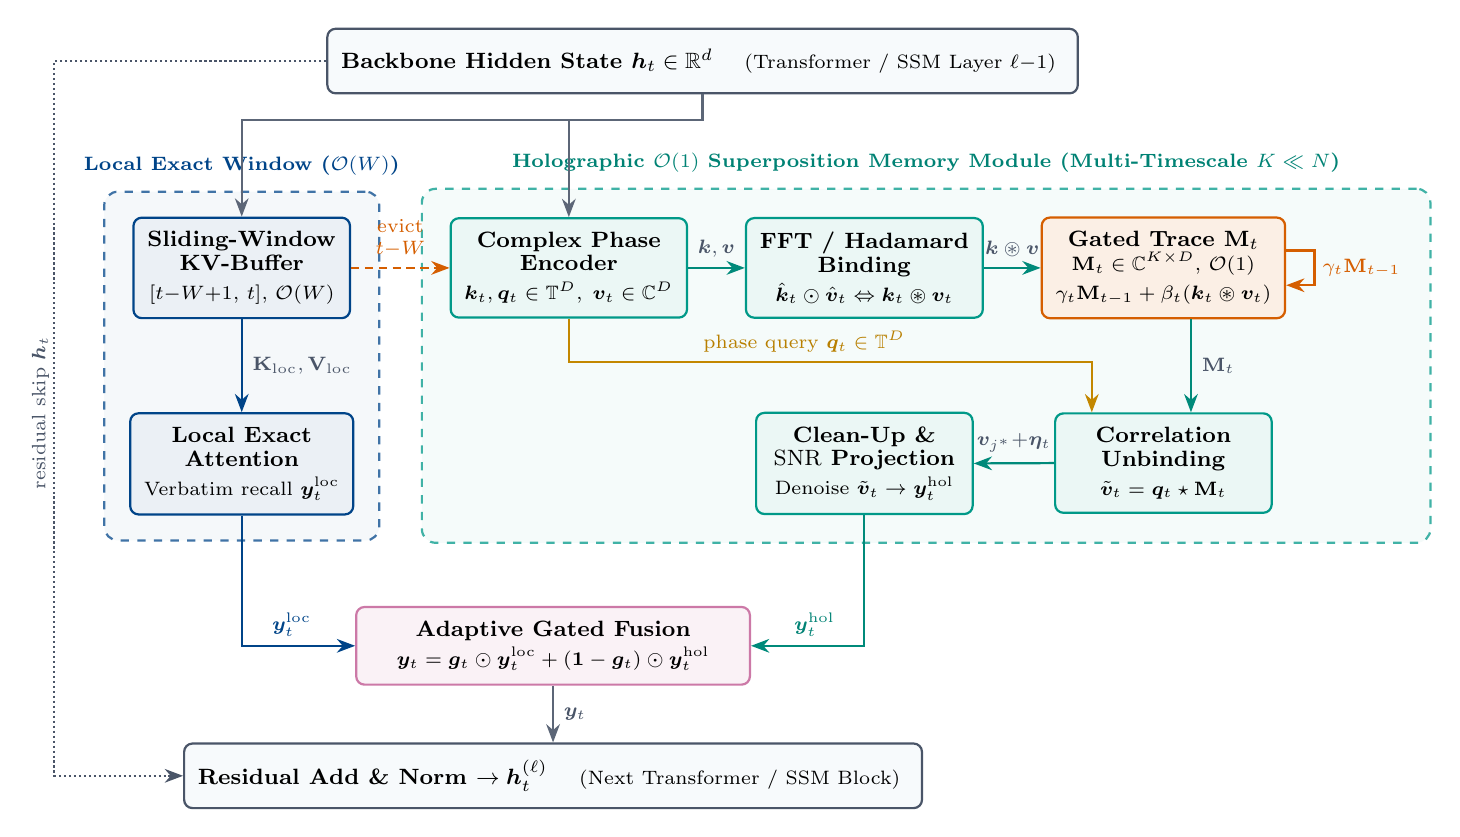
\begin{tikzpicture}[
    font=\footnotesize,
    >=Stealth,
    node distance=0.95cm and 0.72cm,
    % Base block styles
    baseblock/.style={
        rectangle,
        rounded corners=3pt,
        draw=#1,
        fill=#1!8,
        thick,
        align=center,
        inner sep=5pt,
        minimum height=1.18cm,
        text=black
    },
    io/.style={
        baseblock=okabeSlate,
        fill=okabeLightBg,
        minimum width=5.6cm,
        minimum height=0.82cm
    },
    localnode/.style={
        baseblock=okabeNavy,
        minimum width=2.75cm
    },
    holonode/.style={
        baseblock=okabeTeal,
        minimum width=2.75cm
    },
    memnode/.style={
        baseblock=okabeCoral,
        fill=okabeCoral!10,
        minimum width=2.85cm
    },
    fusenode/.style={
        baseblock=okabePurple,
        fill=okabePurple!10,
        minimum width=5.0cm,
        minimum height=0.88cm
    },
    % Container styles
    panel/.style={
        rectangle,
        rounded corners=5pt,
        draw=#1!75,
        fill=#1!4,
        dashed,
        thick,
        inner sep=9pt
    },
    % Arrow styles
    flow/.style={->, thick, draw=okabeSlate!90},
    holoflow/.style={->, thick, draw=okabeTeal!90!black},
    evictflow/.style={->, thick, densely dashed, draw=okabeCoral},
    queryflow/.style={->, thick, draw=okabeAmber!85!black},
    skipflow/.style={->, thick, densely dotted, draw=okabeSlate},
    edgelabel/.style={font=\scriptsize, text=okabeSlate, inner sep=1.5pt}
]

% ------------------------------------------------------------------------------
% Row 1: Local Exact Buffer & Holographic Write Pipeline
% ------------------------------------------------------------------------------
\node[localnode] (buf) {%
    \textbf{Sliding-Window}\\[-1pt]
    \textbf{KV-Buffer}\\[1pt]
    {\scriptsize $[t{-}W{+}1,\,t]$, $\bigo{W}$}
};

\node[holonode, right=1.25cm of buf] (enc) {%
    \textbf{Complex Phase}\\[-1pt]
    \textbf{Encoder}\\[1pt]
    {\scriptsize $\vect{k}_t,\vect{q}_t \in \mathbb{T}^D,\; \vect{v}_t \in \C^D$}
};

\node[holonode, right=0.72cm of enc] (bind) {%
    \textbf{FFT / Hadamard}\\[-1pt]
    \textbf{Binding}\\[1pt]
    {\scriptsize $\hat{\vect{k}}_t \hadamard \hat{\vect{v}}_t \Leftrightarrow \vect{k}_t \cconv \vect{v}_t$}
};

\node[memnode, right=0.72cm of bind] (mem) {%
    \textbf{Gated Trace $\mat{M}_t$}\\[-1pt]
    {\scriptsize $\mat{M}_t \in \C^{K \times D}$, $\bigo{1}$}\\[1pt]
    {\scriptsize $\gamma_t \mat{M}_{t-1} + \beta_t (\vect{k}_t \cconv \vect{v}_t)$}
};

% ------------------------------------------------------------------------------
% Row 2: Local Exact Attention & Holographic Read / Clean-Up Pipeline
% ------------------------------------------------------------------------------
\node[localnode, below=1.18cm of buf] (attn) {%
    \textbf{Local Exact}\\[-1pt]
    \textbf{Attention}\\[1pt]
    {\scriptsize Verbatim recall $\vect{y}_t^{\mathrm{loc}}$}
};

\node[holonode, below=1.18cm of bind] (cleanup) {%
    \textbf{Clean-Up \&}\\[-1pt]
    \textbf{$\SNR$ Projection}\\[1pt]
    {\scriptsize Denoise $\tilde{\vect{v}}_t \to \vect{y}_t^{\mathrm{hol}}$}
};

\node[holonode, below=1.18cm of mem] (unbind) {%
    \textbf{Correlation}\\[-1pt]
    \textbf{Unbinding}\\[1pt]
    {\scriptsize $\tilde{\vect{v}}_t = \vect{q}_t \ccorr \mat{M}_t$}
};

% ------------------------------------------------------------------------------
% Top Input & Bottom Fusion / Residual Backbone Interface
% ------------------------------------------------------------------------------
\coordinate (midTop) at ($(buf.north)!0.5!(mem.north)$);
\node[io, above=1.55cm of midTop] (input) {%
    \textbf{Backbone Hidden State $\vect{h}_t \in \R^{d}$} \quad
    {\scriptsize (Transformer / SSM Layer $\ell{-}1$)}
};

\coordinate (midBot) at ($(attn.south)!0.5!(cleanup.south)$);
\node[fusenode, below=1.15cm of midBot] (fusion) {%
    \textbf{Adaptive Gated Fusion}\\[1pt]
    {\scriptsize $\vect{y}_t = \vect{g}_t \hadamard \vect{y}_t^{\mathrm{loc}} + (\vect{1}-\vect{g}_t) \hadamard \vect{y}_t^{\mathrm{hol}}$}
};

\node[io, below=0.72cm of fusion] (output) {%
    \textbf{Residual Add \& Norm $\to \vect{h}_t^{(\ell)}$} \quad
    {\scriptsize (Next Transformer / SSM Block)}
};

% ------------------------------------------------------------------------------
% Background Shaded Pathway Panels
% ------------------------------------------------------------------------------
% Recurrent multi-timescale self-loop on Gated Trace M_t (coordinate included in fit)
\coordinate (memloop) at ($(mem.east)+(1.48cm,0)$);
\begin{scope}[on background layer]
    \node[panel=okabeNavy, fit=(buf)(attn),
          label={[font=\scriptsize\bfseries, text=okabeNavy, yshift=2pt]above:Local Exact Window ($\bigo{W}$)}]
          (localpanel) {};

    \node[panel=okabeTeal, fit=(enc)(bind)(mem)(cleanup)(unbind)(memloop),
          inner sep=10pt,
          label={[font=\scriptsize\bfseries, text=okabeTeal!85!black, yshift=2pt]above:Holographic $\bigo{1}$ Superposition Memory Module (Multi-Timescale $K \ll N$)}]
          (holopanel) {};
\end{scope}

% ------------------------------------------------------------------------------
% Signal Routing & Connections
% ------------------------------------------------------------------------------
% Input splits to Local Buffer and Holographic Encoder
\coordinate (splitPt) at ($(input.south)+(0,-0.32cm)$);
\draw[flow] (input.south) -- (splitPt) -| (buf.north);
\draw[flow] (splitPt) -| (enc.north);

% Local exact pathway
\draw[flow, draw=okabeNavy] (buf.south) -- node[edgelabel, right=2pt] {$\mat{K}_{\mathrm{loc}}, \mat{V}_{\mathrm{loc}}$} (attn.north);

% Eviction handoff from sliding window into holographic encoder
\draw[evictflow] (buf.east) -- node[edgelabel, text=okabeCoral, above=2pt, align=center] {evict\\$t{-}W$} (enc.west);

% Holographic write path: Encoder -> Binding -> Gated Trace
\draw[holoflow] (enc.east) -- node[edgelabel, above=2pt] {$\vect{k},\vect{v}$} (bind.west);
\draw[holoflow] (bind.east) -- node[edgelabel, above=2pt] {$\vect{k} \cconv \vect{v}$} (mem.west);

% Recurrent multi-timescale self-loop on Gated Trace M_t
\draw[holoflow, draw=okabeCoral]
    ($(mem.east)+(0,0.22cm)$)
    -- ++(0.36cm,0)
    |- node[edgelabel, text=okabeCoral, pos=0.25, right=1pt] {$\gamma_t \mat{M}_{t-1}$}
    ($(mem.east)+(0,-0.22cm)$);

% Holographic read path: Gated Trace -> Correlation Unbinding -> Clean-Up
\draw[holoflow] ($(mem.south)+(0.35cm,0)$) -- node[edgelabel, right=2pt] {$\mat{M}_t$} ($(unbind.north)+(0.35cm,0)$);

% Query routing from Encoder through inter-row corridor to Unbinding (zero crossings)
\coordinate (qCorridor) at ($(enc.south)+(0,-0.55cm)$);
\coordinate (qEntry) at ($(unbind.north west)+(0.48cm,0)$);
\draw[queryflow]
    (enc.south)
    -- (qCorridor)
    -- node[edgelabel, text=okabeAmber!80!black, above=1.5pt, pos=0.45] {phase query $\vect{q}_t \in \mathbb{T}^D$}
    (qCorridor -| qEntry)
    -- (qEntry);

% Unbinding -> Clean-Up
\draw[holoflow] (unbind.west) -- node[edgelabel, above=2pt] {$\vect{v}_{j^*} {+} \vect{\eta}_t$} (cleanup.east);

% Clean-Up & Local Attention -> Adaptive Fusion Gate
\draw[flow, draw=okabeNavy]
    (attn.south) |- node[edgelabel, text=okabeNavy, pos=0.72, above=1.5pt] {$\vect{y}_t^{\mathrm{loc}}$}
    (fusion.west);

\draw[holoflow]
    (cleanup.south) |- node[edgelabel, text=okabeTeal!85!black, pos=0.72, above=1.5pt] {$\vect{y}_t^{\mathrm{hol}}$}
    (fusion.east);

% Fusion -> Residual Add & Norm
\draw[flow] (fusion.south) -- node[edgelabel, right=2pt] {$\vect{y}_t$} (output.north);

% Outer left residual skip connection from Backbone Input to Add & Norm
\coordinate (skipRail) at ($(localpanel.west)+(-0.62cm,0)$);
\coordinate (skipTop) at (input.west -| skipRail);
\coordinate (skipBot) at (output.west -| skipRail);
\draw[skipflow]
    (input.west)
    -- (skipTop)
    -- node[edgelabel, midway, rotate=90, above=2pt] {residual skip $\vect{h}_t$}
    (skipBot)
    -- (output.west);

\end{tikzpicture}
}
    \caption{Conceptual blueprint of a future hybrid foundation-model block combining a bounded local exact sliding-window attention buffer ($\bigo{W}$ memory for verbatim local recall) with a parallel Holographic $\bigo{1}$ Superposition Memory Module. Tokens evicted from the sliding window at step $t-W$ are mapped directly onto spectral-torus phasor keys $\hat{\vect{k}}_t \in \mathbb{T}^D$ and spectral values $\hat{\vect{v}}_t \in \C^D$, bound in $\bigo{KD}$ via elementwise Hadamard modulation ($\hat{\vect{k}}_t \hadamard \hat{\vect{v}}_t \leftrightarrow \vect{k}_t \cconv \vect{v}_t$), and accumulated into a multi-timescale gated spectral trace $\hat{\mat{M}}_t \in \C^{K \times D}$. Incoming spectral queries $\hat{\vect{q}}_t \in \mathbb{T}^D$ retrieve superposed associations via conjugate Hadamard unbinding ($\conj{\hat{\vect{q}}_t} \hadamard \hat{\mat{M}}_t \leftrightarrow \vect{q}_t \ccorr \mat{M}_t$), followed by crosstalk clean-up and adaptive gated fusion with the local exact attention output $\vect{y}_t^{\mathrm{loc}}$.}
    \label{fig:hybrid_arch}
\end{figure}

\paragraph{Learned Phase Keys, Generalized RoPE, and Key Orthogonalization.}
A particularly promising theoretical bridge links holographic KV-caching to Rotary Position Embeddings (RoPE)~\cite{SU_2024_ROPE}.
RoPE applies block-diagonal $2\times 2$ orthogonal rotations---isomorphic to elementwise multiplication by unit-modulus complex phasors $\exp(i m \theta_j)$---so that inner products depend solely on relative phase offsets $\exp(i(m-n)\theta_j)$.
From the perspective of Fourier Holographic Reduced Representations (FHRR)~\cite{PLATE_1995_HRR,SCHLEGEL_VSA_COMPARISON}, RoPE is a special case of \emph{data-independent positional phase binding}.
Holographic KV-caches generalize this mechanism in two directions: first, by learning \emph{content- and context-dependent spectral phase rotations} $\hat{\vect{k}}_t = \exp(i \vect{\phi}(\vect{h}_t)) \in \mathbb{T}^D$ coupled with selective input-dependent decay gates (unifying unitary complex recurrence~\cite{ARJOVSKY_2016_URNN} with selective SSM gating~\cite{GU_SSM_S4_MAMBA}); and second, by introducing \emph{interference-minimizing key orthogonalization}.
Under unregularized random keys, crosstalk variance scales as $\bigo{N_{\mathrm{eff}}/D}$.
However, incorporating a mutual-coherence auxiliary penalty $\mathcal{L}_{\mathrm{coh}} = \sum_{j \neq j'} \abs{\inner{\hat{\vect{k}}_j}{\hat{\vect{k}}_{j'}}}^2$ alongside sparse content-based slot routing (assigning semantically distinct keys to disjoint subsets of the $K$ memory slots via phase hashing) drives keys toward quasi-orthogonal Welch-bound constellations, substantially increasing usable context capacity without enlarging $D$.

% ==============================================================================
\subsection{Hallucination-Reduced and Verifiable Neuro-Symbolic Reasoning}\label{sec:potentials:reasoning}
% ==============================================================================

\paragraph{Explicit Algebraic Binding vs.\ Implicit Statistical Entanglement.}
A primary structural driver of hallucinations in dense Large Language Models (LLMs) is the lack of explicit variable binding.
In standard dense networks, factual associations, entity attributes, and contextual predicates are stored in polysemantic neurons via implicit, unstructured feature superposition~\cite{ELHAGE_2022_SUPERPOSITION}.
Without an algebraic operator that separates \emph{roles} (relations, attributes, slots) from \emph{fillers} (entities, values)~\cite{SMOLENSKY_1990_TPR}, co-occurring entities in a prompt or training corpus become statistically entangled---producing characteristic failure modes such as attribute swapping (assigning Entity A's property to Entity B), entity conflation, and fluent but factually ungrounded confabulation.

Holographic neuro-symbolic representations address this binding problem structurally by encoding relational knowledge through explicit recursive role--filler binding~\cite{PLATE_1995_HRR,NICKEL_2016_HOLE,HERSCHE_2023_NVSA}.
Specifically, an entity record $e_a$ possessing $M$ typed attributes $\{(\vect{r}_m, \vect{f}_{a,m})\}_{m=1}^M$ is composed as a bound superposition $\vect{s}_a = \sum_{m=1}^{M} \vect{r}_m \cconv \vect{f}_{a,m}$, and a multi-entity discourse state bundles distinct entities under entity-identifier keys $\vect{p}_a \in \mathbb{T}^D$:
\begin{equation}\label{eq:neuro_symbolic_bundle}
    \vect{m}_{\mathrm{ctx}} = \sum_{a=1}^{A} \vect{p}_a \cconv \left(\sum_{m=1}^{M} \vect{r}_m \cconv \vect{f}_{a,m}\right).
\end{equation}
Because circular convolution distributes over bundling and maps distinct role--filler pairs into mutually quasi-orthogonal subspaces ($\inner{\vect{p}_a \cconv \vect{r}_m \cconv \vect{f}_{a,m}}{\vect{p}_b \cconv \vect{r}_{m'} \cconv \vect{f}_{b,m'}} \approx 0$ whenever $(a,m) \neq (b,m')$), querying attribute $m$ of entity $a$ via composite unbinding $(\vect{p}_a \cconv \vect{r}_m) \ccorr \vect{m}_{\mathrm{ctx}}$ algebraically isolates $\vect{f}_{a,m}$ rather than interpolating across statistically correlated attributes of entity $b$.
When multiple compositional factors are simultaneously unknown---as in analogical mapping, visual--symbolic reasoning, or multi-hop relational inference---resonator networks~\cite{FRADY_2020_RESONATOR,KENT_2020_RESONATOR} iteratively factorize the composite holographic vector across codebooks in parallel, avoiding the combinatorial search explosion of classical symbolic engines while preserving strict compositional integrity.

\paragraph{Intrinsic Epistemic Uncertainty via Crosstalk and $\SNR$ Diagnostics.}
Beyond preventing attribute entanglement, holographic unbinding offers a mathematically transparent mechanism for \emph{epistemic uncertainty quantification}.
Standard autoregressive decoders map unnormalized logits through a softmax layer that forces probability mass to sum to unity even when a query falls entirely outside the model's stored knowledge, fostering overconfident hallucinations.
In contrast, the raw complex readout $\tilde{\vect{v}}_q = \vect{q} \ccorr \vect{m}$ exhibits starkly distinct geometric statistics for in-memory versus out-of-memory queries.
Let $\mathcal{C} = \{\vect{c}_1, \dots, \vect{c}_V\} \subset \C^D$ denote a normalized clean-up codebook of candidate symbols or concept prototypes.
When $\vect{q}$ matches a stored key $\vect{k}_{j^*}$ bound to $\vect{c}_{u^*}$, the matched inner product concentrates around the coherent signal amplitude $A$, whereas all non-matching prototypes register zero-mean crosstalk with variance proportional to $N/D$.
Conversely, when $\vect{q}$ is unstored (out-of-memory) or suffers severe capacity collision, $\tilde{\vect{v}}_q$ collapses entirely into isotropic crosstalk noise $\vect{\eta}_q$, producing flat similarity scores across $\mathcal{C}$ and dispersed phase angles.

This dichotomy can be operationalized via a dimensionless \emph{retrieval coherence diagnostic} (an empirical peak-to-sidelobe $\SNR$ estimator):
\begin{equation}\label{eq:coherence_metric}
    \rho_{\mathrm{coh}}(\tilde{\vect{v}}_q)
    = \frac{\max_{u \in \{1,\dots,V\}} \abs{\inner{\tilde{\vect{v}}_q}{\vect{c}_u}}}
           {\sqrt{\frac{1}{V-1} \sum_{u \neq u^*} \abs{\inner{\tilde{\vect{v}}_q}{\vect{c}_u}}^2}},
    \qquad u^* = \arg\max_{u} \abs{\inner{\tilde{\vect{v}}_q}{\vect{c}_u}}.
\end{equation}
For fixed $(D, N, V)$, the null distribution of $\rho_{\mathrm{coh}}$ under pure crosstalk noise admits analytical characterization via extreme-value statistics of complex Gaussian projections~\cite{FRADY_CAPACITY_VSA}.
Consequently, whenever $\rho_{\mathrm{coh}}(\tilde{\vect{v}}_q)$ falls below a calibrated decision threshold $\tau_{\mathrm{abs}}$, the model possesses an intrinsic, zero-extra-forward-pass signal indicating an unstored query or retrieval collision---enabling principled abstention, verification-seeking tool calls, or multi-step resonator refinement instead of ungrounded generation.

\paragraph{External Verifiable Holographic Indices.}
A highly practical pathway toward hallucination-reduced AI decouples parametric linguistic fluency from mutable factual storage by pairing frozen foundation models with \emph{external, auditable holographic memory indices}.
Unlike parametric model editing---which frequently induces unintended ripple effects across unrelated facts---or dense vector databases that require periodic graph re-indexing, an external holographic index inherits the linearity and commutativity of bundling.
Inserting a newly verified fact triple $(\vect{k}_{\mathrm{new}}, \vect{v}_{\mathrm{new}})$ or retracting a deprecated or erroneous record requires a single $\bigo{D}$ additive operation:
\begin{equation}\label{eq:holo_edit}
    \vect{m}' = \vect{m} + \vect{k}_{\mathrm{new}} \cconv \vect{v}_{\mathrm{new}} - \vect{k}_{\mathrm{old}} \cconv \vect{v}_{\mathrm{old}},
\end{equation}
without gradient retraining or index reconstruction.
Moreover, provenance and temporal validity metadata can be co-bound into each record via dedicated role keys (e.g., $\vect{r}_{\mathrm{src}} \cconv \vect{f}_{\mathrm{doc}} + \vect{r}_{\mathrm{time}} \cconv \vect{f}_{\mathrm{date}}$), enabling every retrieved assertion to be cryptographically or symbolically audited back to its authoritative source.

% ==============================================================================
\subsection{Continual Learning via Orthogonal Phase Subspaces}\label{sec:potentials:continual}
% ==============================================================================

\paragraph{Context-Keyed Parameter Superposition.}
Catastrophic forgetting arises in gradient-trained neural networks because updating shared synaptic weights for a novel task $\tau$ directly overwrites parameter configurations critical to previously learned tasks $1, \dots, \tau - 1$.
Conventional mitigations---such as quadratic parameter-importance regularization (e.g., Elastic Weight Consolidation~\cite{KIRKPATRICK_2017_EWC}), episodic data replay, or dynamic architectural expansion---either restrict plasticity as task count grows, raise privacy and storage costs, or scale memory linearly with the number of tasks $T$.
Holographic superposition reframes continual learning as \emph{parameter-space multiplexing}: building on Cheung et al.'s Parameter Superposition (PSP) framework~\cite{HOLOGRAPHIC_CONTINUAL_LEARNING}, which multiplexes multiple task models inside a single fixed-dimensional parameter tensor via context-specific diagonal binary or complex phase keys, we formulate continual adaptation in terms of unitary complex phase-key binding.
Extending PSP to complex spectral-torus adapters makes the interplay between exact orthogonal subspace partitioning, quasi-orthogonal interference scaling, and phase-coherence task routing analytically explicit.

Consider a complex-valued linear transformation (or a low-rank adaptation module augmenting a frozen foundation weight matrix) with task-specific weight matrices $\mat{W}_\tau \in \C^{d_{\mathrm{out}} \times d_{\mathrm{in}}}$ for tasks $\tau = 1, \dots, T$.
Assigning each task a diagonal unitary phase-key operator $\mat{C}_\tau = \operatorname{diag}(\vect{c}_\tau)$ with $\vect{c}_\tau \in \mathbb{T}^{d_{\mathrm{in}}}$, all $T$ tasks are superposed into a single shared weight matrix of constant parameter budget $P = d_{\mathrm{out}} d_{\mathrm{in}}$:
\begin{equation}\label{eq:continual_superposition}
    \mat{W}_{\mathrm{sup}} = \sum_{\tau=1}^{T} \mat{W}_\tau \mat{C}_\tau.
\end{equation}
At inference time on task $\tau$, modulating the input activation $\vect{x} \in \C^{d_{\mathrm{in}}}$ by the conjugate key $\mat{C}_\tau\herm = \operatorname{diag}(\conj{\vect{c}}_\tau)$ recovers the target linear map plus an inter-task crosstalk residual:
\begin{equation}\label{eq:continual_readout}
    \hat{\vect{y}}_\tau
    = \mat{W}_{\mathrm{sup}} \mat{C}_\tau\herm \vect{x}
    = \mat{W}_\tau \vect{x}
      + \underbrace{\sum_{\tau' \neq \tau} \mat{W}_{\tau'} \bigl(\mat{C}_{\tau'} \mat{C}_\tau\herm\bigr) \vect{x}}_{\vect{\xi}_\tau \text{ (inter-task crosstalk)}}.
\end{equation}
Critically, whereas coordinate-wise subtraction of two unprojected weight matrices would experience $\bigo{1}$ per-entry interference, the linear layer's fan-in summation coherently integrates the target signal $\mat{W}_\tau \vect{x}$ while incoherently averaging the phase-randomized cross-terms $\mat{W}_{\tau'}(\mat{C}_{\tau'}\mat{C}_\tau\herm)\vect{x}$.
When the relative phases $\arg(c_{\tau',j}\conj{c}_{\tau,j})$ are independent and uniformly distributed on $[0, 2\pi)$ across input coordinates $j \in \{1,\dots,d_{\mathrm{in}}\}$ and tasks have comparable weight energy $\sigma_w^2$, the per-output interference variance scales as $\E[\abs{\xi_{\tau,i}}^2] \propto (T - 1)\, d_{\mathrm{in}}\, \sigma_w^2 \sigma_x^2$.
Under a \emph{weight--activation alignment} assumption---namely, that gradient training aligns active rows $\vect{w}_{\tau,i}$ of $\mat{W}_\tau$ with task-$\tau$ feature activations $\vect{x}$ such that $\abs{(\mat{W}_\tau \vect{x})_i}^2 = \kappa_\tau \norm{\vect{w}_{\tau,i}}_2^2 \norm{\vect{x}}_2^2 \asymp \kappa_\tau\, d_{\mathrm{in}}^2\, \sigma_w^2 \sigma_x^2$ with alignment factor $\kappa_\tau = \Omega(1)$ across the active fan-in (whereas unaligned random features satisfy $\kappa_\tau = \bigo{d_{\mathrm{in}}^{-1}}$ and gain no width advantage)---the coherently aligned task response scales quadratically in $d_{\mathrm{in}}$.
Consequently, in this aligned feature-learning regime, the effective task signal-to-interference ratio satisfies $\SNR_{\mathrm{task}} \propto \kappa_\tau d_{\mathrm{in}} / (T - 1)$, mirroring the fundamental holographic scaling law and guaranteeing that wider layers absorb proportionally more tasks without catastrophic collapse.

\paragraph{Orthogonal Phase Subspaces, Capacity Budgeting, and Task-Free Routing.}
The scaling of \eqref{eq:continual_readout} naturally partitions holographic continual learning into two distinct capacity regimes governed by the ambient dimensionality $D$ and the effective subspace dimension $S$ required per task:
\begin{enumerate}
    \item \textbf{Exact Interference-Free Regime ($T \le \lfloor D/S \rfloor$):}
    By restricting task representations or Fourier-domain adapters to mutually orthogonal complex phase subspaces---for example, partitioning spectral bins or enforcing unitary block projections $\mat{P}_\tau \mat{P}_{\tau'}\herm = \mat{0}$ for $\tau \neq \tau'$---inter-task crosstalk vanishes identically ($\vect{\xi}_\tau = \vect{0}$).
    New tasks incur zero forgetting of prior tasks while still sharing a unified forward computation graph.
    \item \textbf{Graceful Quasi-Orthogonal Superposition Regime ($T > \lfloor D/S \rfloor$):}
    Once exact orthogonal capacity is exhausted, additional tasks are accommodated by relaxing strict orthogonality to quasi-orthogonal tight frames or random unit-phasor keys $\vect{c}_\tau \in \mathbb{T}^D$ approaching the Welch coherence bound.
    Rather than suffering sudden catastrophic forgetting, accuracy across the task ensemble degrades smoothly and predictably as a function of the task-to-dimension ratio $T S / D$, enabling explicit capacity budgeting before deployment.
\end{enumerate}

Two open algorithmic opportunities further strengthen this paradigm for autonomous lifelong learners.
First, in \emph{task-free} continual learning where the task identifier $\tau$ is unavailable at test time, the context key $\vect{c}_\tau$ can itself be inferred dynamically by querying a lightweight holographic task-index memory or by selecting the candidate key $\vect{c}_\tau$ that maximizes output phase coherence or minimizes prediction entropy across candidate routings~\cite{HOLOGRAPHIC_CONTINUAL_LEARNING}.
Second, periodic \emph{phase-orthogonal consolidation}---akin to sleep-phase memory consolidation---can detect redundant or correlated task subspaces, distill shared skills into an unkeyed base weight $\mat{W}_0$, and re-orthogonalize residual task keys to reclaim holographic headroom across indefinite non-stationary streams.

% ==============================================================================
\subsection{Open Scaling Bottlenecks and Research Frontier}\label{sec:potentials:challenges}
% ==============================================================================

Realizing the architectural visions outlined in Sections~\ref{sec:potentials:kvcache}--\ref{sec:potentials:continual} at frontier scale requires confronting three deep technical bottlenecks spanning information theory, optimization and systems engineering, and empirical methodology.

\paragraph{The Crosstalk Ceiling ($\SNR \propto D/N$) and Memory--Fidelity Trade-Offs.}
No linear superposition scheme can circumvent Shannon's information-theoretic capacity limits.
A complex vector $\vect{m} \in \C^D$ quantized to $b$ bits per real component carries at most $2 D b$ bits of entropy; consequently, attempting lossless verbatim recall of $N$ arbitrary high-entropy items from a single dense holographic trace inevitably encounters the crosstalk ceiling $\SNR \propto D / N$~\cite{PLATE_1995_HRR,FRADY_CAPACITY_VSA}.
For modern language models where $N$ may exceed $10^6$ tokens while layer dimensions remain $D \sim 10^3\text{--}10^4$, naive single-trace dense superposition operates deep in the sub-unit $\SNR$ regime.
Overcoming this ceiling requires moving beyond monolithic dense bundling along three research axes:
(i) \emph{semantic--verbatim decoupling}, using holographic traces strictly for lossy semantic gist, entity--relation state, and coarse episodic pointers while delegating exact string copying to local windows or sparse exact caches;
(ii) \emph{sparse and block-structured holographic codes}~\cite{SCHLEGEL_VSA_COMPARISON,KLEYKO_VSA_SURVEY}, wherein binding operates over block-sparse segmented phasors that restrict crosstalk to active blocks and dramatically improve bits-per-dimension efficiency; and
(iii) \emph{adaptive nonlinear clean-up memories}, coupling holographic readouts with dense associative memories (modern Hopfield networks~\cite{RAMSAUER_MODERN_HOPFIELD}) or iterative resonator networks~\cite{FRADY_2020_RESONATOR} that trade bounded iterative compute for near-exponential codebook separation.

\paragraph{Optimization and Systems Barriers for Phase-Coupled Deep Networks.}
Scaling complex-valued and phase-coupled holographic layers to multi-billion-parameter networks exposes severe optimization and hardware-systems friction~\cite{BASSEY_CVNN_SURVEY,TRABELSI_2018_DCN}.
Although Wirtinger calculus provides exact gradients for real-valued loss functions of complex parameters, backpropagation through deep chains of circular convolutions, correlations, and periodic phase encodings $\exp(i\vect{\phi})$ suffers from phase-wrapping discontinuities ($\phi \equiv \phi + 2\pi$) and highly oscillatory, non-convex loss surfaces with abundant local minima.
Preserving unit-modulus phasor norms ($\vect{k} \in \mathbb{T}^D$) without killing gradient flow demands specialized manifold optimizers, complex-aware normalization layers, and phase-preserving nonlinearities (such as $\mathrm{modReLU}$ or gated spectral filtering) whose stability at 100-layer depths remains far less understood than real-valued pre-norm Transformer recipes.

Compounding these optimization hurdles is an acute \emph{hardware lottery} penalty~\cite{HOOKER_2021_HARDWARE_LOTTERY}.
Contemporary AI accelerators---notably GPU Tensor Cores and systolic TPUs---are heavily specialized for low-precision real-valued general matrix multiplication (GEMM in \texttt{BF16}, \texttt{FP16}, and \texttt{FP8}).
By contrast, batched small-to-medium FFTs for circular convolution, fused complex Hadamard recurrences, and low-precision quantized phase arithmetic exhibit poor arithmetic intensity and limited kernel fusion on commodity GPUs, often erasing the asymptotic FLOP advantages of $\bigo{D \log D}$ binding in wall-clock latency.
Closing this systems gap will require both hardware-aware digital kernels (e.g., fused Triton/CUDA complex-recurrence and spectral-convolution kernels analogous to FlashAttention and Mamba scan primitives) and tight algorithm--hardware co-design with native coherent photonic and diffractive optical accelerators~\cite{WETZSTEIN_2020_OPTICAL_AI,MCMAHON_2023_PHYSICS_OPTICAL_NN}, where complex phase modulation and interference execute natively at the speed of light.

\paragraph{Need for Standardized Cross-Paradigm Benchmarks.}
Finally, empirical progress in holographic neural networks and VSAs has historically been impeded by fragmented evaluation practices.
Many studies validate capacity or reasoning claims on small-scale synthetic tasks (e.g., few-hundred-item key--value dictionaries, low-dimensional classification, or bespoke cognitive puzzles) without direct, compute-matched comparisons against modern Transformers, SSMs, and Hopfield baselines.
To establish scientific consensus on where holographic superposition genuinely outperforms competing paradigms, the community needs a unified, open benchmark suite spanning four standardized evaluation pillars:
\begin{enumerate}
    \item \textbf{Long-Horizon Associative Recall and Selective Copying:} Scaling context length $N$ from $10^3$ to $10^6$ under fixed memory budgets, disentangling exact verbatim copying from multi-hop semantic aggregation by combining synthetic recall diagnostics (Zoology~\cite{ARORA_2023_ZOOLOGY,JELASSI_2024_REPEAT_AFTER_ME}) with standardized long-context stress tests such as RULER~\cite{HSIEH_2024_RULER} (multi-key/multi-value retrieval, variable tracking, and aggregation) and BABILong~\cite{KURATOV_2024_BABILONG} (multi-hop reasoning over facts buried in million-token distractors). Directly reporting holographic, delta-rule, and hybrid models on these suites exposes the exact crosstalk--capacity frontier beyond short synthetic dictionaries.
    \item \textbf{Compositional Systematicity and Hallucination Calibration:} Evaluating out-of-distribution role--filler recombination, multi-entity attribute binding under distractor density, and abstention calibration (e.g., AUROC and selective risk via $\rho_{\mathrm{coh}}$) on unstored or contradictory queries.
    \item \textbf{Continual Task-Stream Retention:} Measuring average accuracy, backward transfer, and graceful interference curves as a function of the task-to-parameter load ratio $T/P$ under strict parameter and replay constraints.
    \item \textbf{Hardware-Normalized Efficiency and Physical Noise Resilience:} Reporting wall-clock throughput, memory-bandwidth utilization, energy per token ($\mathrm{J/tok}$), and accuracy degradation under realistic low-bit phase quantization, thermal phase drift, and photonic shot-noise perturbations~\cite{WETZSTEIN_2020_OPTICAL_AI,MCMAHON_2023_PHYSICS_OPTICAL_NN}.
\end{enumerate}
Such unified benchmarks---paired with reproducible complex-valued kernel libraries---will convert holographic neural computation from a compelling theoretical paradigm into a rigorously validated pillar of next-generation AI systems.

\section{Conclusion}\label{sec:conclusion}

% ------------------------------------------------------------------------------
\subsection{Synthesis of Key Findings}\label{sec:conclusion:synthesis}
% ------------------------------------------------------------------------------

Tracing the trajectory from Dennis Gabor's optical wave interference~\cite{GABOR_1948_HOLOGRAPHY} and John Sutherland's complex-valued Holographic Neural Networks~\cite{SUTHERLAND_1990_HNN}, through Tony Plate's Holographic Reduced Representations~\cite{PLATE_1995_HRR} and Pentti Kanerva's Hyperdimensional Computing~\cite{KANERVA_2009_HDC}, to contemporary Complex-Valued Neural Networks~\cite{BASSEY_CVNN_SURVEY}, Fourier token mixers~\cite{LEE_THORP_FNET}, linear attention~\cite{KATHAROPOULOS_2020_LINEAR_TRANSFORMER}, and State-Space Models~\cite{GU_SSM_S4_MAMBA} reveals a remarkably unified mathematical, architectural, and physical picture.
Three core takeaways synthesize the findings of this survey.

\paragraph{Mathematical Synthesis: Distributed Phase Superposition and the $\SNR \propto D/N$ Law.}
Across nearly eight decades of seemingly disparate formulations, holographic neural computation rests on a single algebraic core formalized in Section~\ref{sec:math}: mapping structured data into high-dimensional complex phasor spaces ($\C^D$, and ideally the unitary torus $\mathbb{T}^D$) where quasi-orthogonality supports exponentially many distinct symbols (Proposition~\ref{prop:quasi_ortho}), binding via circular convolution $\cconv$ or $\bigo{D}$ spectral Hadamard phase addition $\hadamard$ preserves dimensionality (Proposition~\ref{prop:conv_thm}), bundling superposes $N$ associations into a fixed-size trace, and circular correlation $\ccorr$ unbinds queried entries as the exact Hilbert-space adjoint (Lemma~\ref{lem:ccorr_props}).
This algebraic compression trades the $\bigo{ND}$ storage of explicit tables for $\bigo{1}$ memory with respect to $N$, incurring zero-mean additive crosstalk noise $\vect{\eta}$ governed universally by $\SNR = \Theta(D/N)$ (Theorem~\ref{thm:snr_capacity}).
Crucially, unitary complex phasors eliminate spectral self-distortion and reject orthogonal quadrature noise, securing a factor-of-two ($3\,\mathrm{dB}$) discrimination $\SNR$ advantage over real Gaussian HRR at equal width $D$, while clean-up projection onto a discrete codebook $\mathcal{V}$ of size $M$ yields reliable retrieval capacity $N_{\max} = \Theta(D / \ln(M/\delta))$ (Corollary~\ref{cor:cleanup_capacity}).
Rather than an arbitrary heuristic, the Shannon-entropy ceiling of fixed-width traces (Proposition~\ref{prop:superposition_duality}) provides an exact analytical boundary separating compressed semantic recall from lossless verbatim storage.

\paragraph{Architectural Synthesis: Complementarity Over Replacement.}
Our genealogical analysis (Section~\ref{sec:history}) and six-axis cross-paradigm evaluation (Section~\ref{sec:comparison}, Table~\ref{tab:paradigm_comparison}) establish a sharp structural bifurcation across modern AI.
\emph{Non-parametric explicit attention}---encompassing Modern Hopfield Networks~\cite{RAMSAUER_MODERN_HOPFIELD} and softmax Transformers~\cite{VASWANI_TRANSFORMER}---eliminates additive crosstalk via unfactorable exponential selectivity, achieving lossless verbatim copying and fine-grained disambiguation at the cost of $\bigo{ND}$ KV-cache growth and $\bigo{N^2}$ pairwise interaction.
\emph{Parametric holographic superposition}---spanning HNNs, HRR/HDC, linear attention, and selective SSMs---delivers constant-memory $\bigo{1}$ state updates, native dimension-preserving role--filler compositionality, one-shot algebraic plasticity, and graceful noise degradation, yet cannot circumvent fixed-state entropy bounds on unstructured verbatim copying~\cite{JELASSI_2024_REPEAT_AFTER_ME,ARORA_2023_ZOOLOGY}.
The decisive architectural conclusion is therefore \emph{complementarity rather than wholesale replacement}: holographic superposition is not a drop-in substitute for exact local attention, but an ideal mathematical substrate for compressed long-horizon semantic memory, structured neuro-symbolic binding, and interference-controlled continual adaptation.
As articulated in Section~\ref{sec:potentials}, hybrid foundation architectures (Figure~\ref{fig:hybrid_arch}) that pair bounded exact sliding-window attention with multi-timescale holographic $\bigo{1}$ memory modules, leverage crosstalk coherence diagnostics ($\rho_{\mathrm{coh}}$) for calibrated epistemic abstention, and multiplex task adapters across orthogonal complex phase subspaces offer a principled pathway toward scalable, verifiable, and lifelong AI.

\paragraph{Hardware Co-Design Synthesis: Matching Algebraic Primitives to Physical Substrates.}
Perhaps the clearest lesson of Section~\ref{sec:applications} (Table~\ref{tab:hardware_substrates}) is that holographic representations achieve their most transformative gains when paired with physical substrates aligned to their algebraic primitives rather than forced onto real-valued GEMM pipelines.
Discrete binary and bipolar VSA specializations collapse binding and similarity to bitwise XOR and popcount, enabling single-pass on-device learning on milliwatt digital microcontrollers and FPGAs~\cite{RAHIMI_HDC_EDGE,KIM_2020_GENIEHD}, while their high-dimensional bit-error resilience ($10\text{--}30\%$ BER tolerance) naturally absorbs conductance drift and stuck-at faults in analog Phase-Change Memory and RRAM in-memory computing crossbars~\cite{KARUNARATNE_2020_PCM_HDC}.
At the continuous end of the spectrum, complex-phasor HNNs and FHRR exhibit a one-to-one physical isomorphism with coherent optical wavefields: passive interference performs bundling, spatial phase masks execute Hadamard binding, spherical lenses compute exact spatial Fourier transforms, and integrated Mach--Zehnder interferometer meshes~\cite{SHEN_PHOTONIC_MZI,CLEMENTS_2016_MZI} alongside free-space diffractive networks ($\text{D}^2\text{NN}$)~\cite{LIN_DIFFRACTIVE_OPTICAL_NN} realize complex unitary transformations at optical carrier speeds~\cite{WETZSTEIN_2020_OPTICAL_AI,MCMAHON_2023_PHYSICS_OPTICAL_NN}.

% ------------------------------------------------------------------------------
\subsection{Outlook for Algorithm--Hardware Co-Design}\label{sec:conclusion:outlook}
% ------------------------------------------------------------------------------

Looking ahead, the convergence of hybrid holographic--Transformer/SSM algorithms with emerging photonic interferometers, diffractive optics, and analog in-memory fabrics signals a rare inflection point in computing.
For decades, algorithmic progress has been shaped by the CMOS GEMM \emph{hardware lottery}~\cite{HOOKER_2021_HARDWARE_LOTTERY}, privileging dense real-valued matrix multiplications that execute efficiently on digital systolic arrays while penalizing complex phase operations, FFT convolutions, and sparse algebraic bindings.
As electronic scaling encounters hard physical ceilings in interconnect energy and off-chip memory bandwidth, computational primitives that operate natively in complex phase space, tolerate analog physical noise, and maintain constant-footprint distributed state are poised to move from niche academic alternatives to first-class architectural building blocks.

Realizing this promise at frontier scale will require coordinated progress across three concrete research priorities:
\begin{enumerate}
    \item \textbf{Scalable Complex-Valued Training Primitives and Hybrid Memory Architectures:}
    The deep learning systems community must overcome phase-wrapping optimization instabilities in deep phase-coupled networks through principled manifold optimization, phase-preserving normalization, and stable Wirtinger recipes~\cite{BASSEY_CVNN_SURVEY,TRABELSI_2018_DCN}. In parallel, bridging the immediate digital hardware gap demands fused GPU/accelerator kernels (analogous to FlashAttention and parallel selective scans) for batched complex FFTs, gated Hadamard recurrences, and hierarchical sliding-window plus holographic $\bigo{1}$ KV-cache blocks (Section~\ref{sec:potentials:kvcache}).
    \item \textbf{Rigorous Capacity, Correlation, and Uncertainty Theory for Learned Non-Orthogonal Keys:}
    Classical VSA capacity theorems assume i.i.d.\ random quasi-orthogonal keys, whereas end-to-end neural encoders inevitably induce semantic clustering and cross-key correlations that bias superposed readouts. Extending the analytical framework of Section~\ref{sec:math} to correlated learned keys---combining mutual-coherence regularization, block-sparse phase codes, resonator/Hopfield clean-up attractors~\cite{FRADY_2020_RESONATOR,RAMSAUER_MODERN_HOPFIELD}, and calibrated $\SNR$-based epistemic uncertainty bounds ($\rho_{\mathrm{coh}}$)---is essential to unlock both high-capacity long-context memory and verifiable, hallucination-resistant neuro-symbolic reasoning (Sections~\ref{sec:potentials:reasoning}--\ref{sec:potentials:continual}).
    \item \textbf{Co-Designed Optical, Analog, and Edge Benchmarks Bridging Theory and Physical Deployment:}
    On the hardware frontier, closing the gap between laboratory photonic prototypes and general-purpose AI accelerators requires amortizing electro-optic conversion (E--O--E) overheads via high-fan-in spatial and wavelength multiplexing, maturing low-power optical nonlinearities, and leveraging non-volatile photonic phase-change materials to eliminate static thermal drift~\cite{WETZSTEIN_2020_OPTICAL_AI,MCMAHON_2023_PHYSICS_OPTICAL_NN}. Simultaneously, the field needs standardized, compute- and energy-normalized cross-paradigm benchmarks spanning long-horizon associative recall, compositional systematicity, continual task retention, and physical noise resilience (Section~\ref{sec:potentials:challenges}).
\end{enumerate}

The journey from optical interference plates to high-dimensional latent superposition has come full circle: mathematical abstractions originally borrowed from wave physics to explain biological associative memory now stand ready to both alleviate the scaling bottlenecks of modern foundation models and guide the architecture of future optical and analog AI hardware.
By uniting rigorous phase-space theory, hybrid neural--symbolic architectures, and physically native execution substrates, holographic neural computation offers a durable blueprint for more energy-efficient, compositional, and resilient artificial intelligence.


% ==============================================================================
% Acknowledgments & AI Assistance Disclosure
% ==============================================================================
\section*{Acknowledgments \& AI Assistance Disclosure}
\phantomsection
\addcontentsline{toc}{section}{Acknowledgments \& AI Assistance Disclosure}

This survey was produced in collaboration with Gemini 4 Neon, which provided significant support in synthesizing the academic literature, formulating the mathematical content, typesetting in LaTeX, and creating the figures. Additional technical editing, reproducibility checks, and exploratory simulation design were assisted by ChatGPT (OpenAI). The author remains responsible for independently verifying all calculations, citations, and reported results prior to submission.

% ==============================================================================
% Bibliography
% ==============================================================================
\bibliographystyle{plain} % Can be switched to IEEEtran, ACM-Reference-Format, etc.
\bibliography{references}

% ==============================================================================
% Appendix A: Reproducible Monte Carlo Simulation Script
% ==============================================================================
\clearpage
\appendix
\section{Reproducible Monte Carlo Simulation Script}\label{app:simulation}

To ensure this survey is fully self-contained and that the empirical discrimination $\SNR^{\mathrm{disc}}$ curves in Figure~\ref{fig:capacity}(a) (corroborating Theorem~\ref{thm:snr_capacity}) can be reproduced directly without external repository access, Listing~\ref{lst:simulate_capacity} provides the complete, verbatim Python/NumPy simulation script (\texttt{figures/simulate\_capacity.py}) used to generate \texttt{figures/capacity\_snr.dat}.
Running \texttt{python figures/simulate\_capacity.py --seed 2026} deterministically regenerates all 17 Monte Carlo operating points across $D \in \{256, 1024, 4096\}$.

\lstinputlisting[style=holoPython, caption={Reproducible Monte Carlo simulation script validating Theorem~\ref{thm:snr_capacity} and generating Figure~\ref{fig:capacity}(a).}, label={lst:simulate_capacity}]{figures/simulate_capacity.py}


\clearpage
\section{Exploratory Correlated-Key Retrieval Stress Test}\label{app:correlated}
The exact FHRR crosstalk analysis in Theorem~\ref{thm:snr_capacity} assumes mutually independent uniform-phase keys and values. To probe one failure mode outside this regime, we additionally evaluate a controlled family of \emph{correlated} keys $K_{n,\omega}=\exp(i(\phi_\omega+\epsilon_{n,\omega}))$, where a random anchor $\phi_\omega$ is shared across the $N$ keys and $\epsilon_{n,\omega}\sim\mathcal N(0,\sigma^2)$. Value vectors remain independent uniform-phase phasors. Each trace is queried using its first stored key; the clean-up dictionary contains all $N$ stored values (not just one independent, unstored distractor). The test uses $D=256$, 500 independent trials per condition and random seed 2026. Results are exploratory estimates, not theoretical guarantees.

\begin{table}[htbp]
\centering
\small
\caption{Correlated-key FHRR stress test. Key similarity is mean normalized real overlap between the first two keys; top-1 recall selects among all $N$ stored values. The margin is target score minus largest competing score (negative implies frequent collision).}
\label{tab:correlated_keys}
\begin{tabular}{rrrrr}
\toprule
$N$ & Phase noise $\sigma$ & Mean key similarity & Top-1 recall & Mean margin \\
\midrule
8 & 0.30 & 0.913 & 0.314 & -0.072 \\
8 & 1.00 & 0.368 & 1.000 & 0.471 \\
8 & 3.00 & -0.003 & 1.000 & 0.835 \\
32 & 0.30 & 0.914 & 0.076 & -0.402 \\
32 & 1.00 & 0.365 & 0.706 & 0.132 \\
32 & 3.00 & -0.002 & 0.962 & 0.496 \\
64 & 0.30 & 0.914 & 0.026 & -0.716 \\
64 & 1.00 & 0.368 & 0.348 & -0.161 \\
64 & 3.00 & -0.000 & 0.666 & 0.167 \\
\bottomrule
\end{tabular}
\end{table}

Strongly correlated keys can defeat reliable discrimination despite fixed-dimensional state size: at $N=32$, the observed top-1 retrieval rate falls from 96.2\% for nearly uncorrelated keys ($\sigma=3$) to 7.6\% for highly correlated keys ($\sigma=0.3$). Unlike the independent-random-codebook setting, the retrieval score for competing stored values now depends on the key--key correlations. The reported accuracies are sensitive to the selected $D$, $N$, noise distribution and clean-up codebook; they do \emph{not} predict downstream language-model performance. The following standalone source reproduces the experiment and prints all nine operating points.

\lstinputlisting[style=holoPython, caption={Exploratory correlated-key stress test; run \texttt{python figures/simulate\_correlated\_keys.py}.}, label={lst:correlated_keys}]{figures/simulate_correlated_keys.py}

\end{document}
